%-----------------------------------
% Define document and include general packages
%-----------------------------------
% Tabellen- und Abkürzungsverzeichnis stehen normalerweise nicht im
% Inhaltsverzeichnis. Gleiches gilt für das Abkürzungsverzeichnis (siehe unten).
% Manche Dozenten bemängeln das. Die Optionen 'listof=totoc,bibliography=totoc'
% geben das Tabellen- und Abkürzungsverzeichnis im Inhaltsverzeichnis (toc=Table
% of Content) aus.
% Da es aber verschiedene Regelungen je nach Dozent geben kann, werden hier
% beide Varianten dargestellt.
%\documentclass[12pt,oneside,titlepage,listof=totoc,bibliography=totoc]{scrartcl}
\documentclass[12pt,oneside,titlepage]{scrartcl}

%-----------------------------------
% Dokumentensprache
%-----------------------------------
%\def\FOMEN{}% Auskommentieren um die Dokumentensprache auf englisch zu ändern
\newif\ifde
\newif\ifen

%-----------------------------------
% Meta informationen
%-----------------------------------
%-----------------------------------
% Meta Informationen zur Arbeit
%-----------------------------------

% Autor
\newcommand{\myAutor}{Christopher Becker}

% Adresse
\newcommand{\myAdresse}{Bahnhofstra\ss e 2 \\ \> \> \> 82211 Herrsching am Ammersee}

% Titel der Arbeit
\newcommand{\myTitel}{Financial optimization of cryptomining data centers by the introduction of Business Intelligence Processes}

% Betreuer
\newcommand{\myBetreuer}{Dr. rer. nat. Michael Colombo}

% Lehrveranstaltung
\newcommand{\myLehrveranstaltung}{Modul Nr. 1}

% Matrikelnummer
\newcommand{\myMatrikelNr}{477668}

% Ort
\newcommand{\myOrt}{München}

% Datum der Abgabe
\newcommand{\myAbgabeDatum}{\today}

% Semesterzahl
\newcommand{\mySemesterZahl}{7}

% Name der Hochschule
\newcommand{\myHochschulName}{FOM Hochschule für Oekonomie \& Management}

% Standort der Hochschule
\newcommand{\myHochschulStandort}{München}

% Studiengang
\newcommand{\myStudiengang}{Business Informatics}

% Art der Arbeit
\newcommand{\myThesisArt}{Bachelor Thesis}

% Zu erlangender akademische Grad
\newcommand{\myAkademischerGrad}{Bachelor of Science (B.Sc.)}

% Firma
\newcommand{\myFirma}{Genesis Group}


\ifdefined\FOMEN
%Englisch
\entrue
\usepackage[english]{babel}
\else
%Deutsch
\detrue
\usepackage[ngerman]{babel}
\fi


\newcommand{\langde}[1]{%
   \ifde\selectlanguage{ngerman}#1\fi}
\newcommand{\langen}[1]{%
   \ifen\selectlanguage{english}#1\fi}
\usepackage[utf8]{luainputenc}
\langde{\usepackage[babel,german=quotes]{csquotes}}
\langen{\usepackage[babel,english=british]{csquotes}}
\usepackage[T1]{fontenc}
\usepackage{fancyhdr}
\usepackage{fancybox}
\usepackage[a4paper, left=4cm, right=2cm, top=4cm, bottom=2cm]{geometry}
\usepackage{graphicx}
\usepackage{colortbl}
\usepackage[capposition=top]{floatrow}
\usepackage{array}
\usepackage{float}      %Positionierung von Abb. und Tabellen mit [H] erzwingen
\usepackage{footnote}
% Darstellung der Beschriftung von Tabellen und Abbildungen (Leitfaden S. 44)
% singlelinecheck=false: macht die Caption linksbündig (statt zentriert)
% labelfont auf fett: (Tabelle x.y:, Abbildung: x.y)
% font auf fett: eigentliche Bezeichnung der Abbildung oder Tabelle
% Fettschrift laut Leitfaden 2018 S. 45
\usepackage[singlelinecheck=false, labelfont=bf, font=bf]{caption}
\usepackage{caption}
\usepackage{enumitem}
\usepackage{amssymb}
\usepackage{mathptmx}
%\usepackage{minted} %Kann für schöneres Syntax Highlighting genutzt werden. ACHTUNG: Python muss installiert sein.
\usepackage[scaled=0.9]{helvet} % Behebt, zusammen mit Package courier, pixelige Überschriften. Ist, zusammen mit mathptx, dem times-Package vorzuziehen. Details: https://latex-kurs.de/fragen/schriftarten/Times_New_Roman.html
\usepackage{courier}
\usepackage{amsmath}
\usepackage[table]{xcolor}
\usepackage{marvosym}			% Verwendung von Symbolen, z.B. perfektes Eurozeichen
\renewcommand\familydefault{\sfdefault}
\usepackage{ragged2e}

% Mehrere Fussnoten nacheinander mit Komma separiert
\usepackage[hang, multiple]{footmisc}
\setlength{\footnotemargin}{1em}

% todo Aufgaben als Kommentare verfassen für verschiedene Editoren
\usepackage{todonotes}

% Verhindert, dass nur eine Zeile auf der nächsten Seite steht
\setlength{\marginparwidth}{2cm}
\usepackage[all]{nowidow}

% Horizontal geteilte Zellen
\newcommand{\specialcell}[2][c]{%
  \begin{tabular}[#1]{@{}c@{}}#2\end{tabular}}

%-----------------------------------
% Farbdefinitionen
%-----------------------------------
\definecolor{darkblack}{rgb}{0,0,0}
\definecolor{dunkelgrau}{rgb}{0.8,0.8,0.8}
\definecolor{hellgrau}{rgb}{0.0,0.7,0.99}
\definecolor{mauve}{rgb}{0.58,0,0.82}
\definecolor{dkgreen}{rgb}{0,0.6,0}

%-----------------------------------
% Pakete für Tabellen
%-----------------------------------
\usepackage{epstopdf}
\usepackage{nicefrac} % Brüche
\usepackage{multirow}
\usepackage{rotating} % vertikal schreiben
\usepackage{mdwlist}
\usepackage{tabularx}% für Breitenangabe

%-----------------------------------
% sauber formatierter Quelltext
%-----------------------------------
\usepackage{listings}
\usepackage{threeparttable}
% JavaScript als Sprache definieren:
\lstdefinelanguage{JavaScript}{
	keywords={break, super, case, extends, switch, catch, finally, for, const, function, try, continue, if, typeof, debugger, var, default, in, void, delete, instanceof, while, do, new, with, else, return, yield, enum, let, await},
	keywordstyle=\color{blue}\bfseries,
	ndkeywords={class, export, boolean, throw, implements, import, this, interface, package, private, protected, public, static},
	ndkeywordstyle=\color{darkgray}\bfseries,
	identifierstyle=\color{black},
	sensitive=false,
	comment=[l]{//},
	morecomment=[s]{/*}{*/},
	commentstyle=\color{purple}\ttfamily,
	stringstyle=\color{red}\ttfamily,
	morestring=[b]',
	morestring=[b]"
}

\lstset{
	%language=JavaScript,
	numbers=left,
	numberstyle=\tiny,
	numbersep=5pt,
	breaklines=true,
	showstringspaces=false,
	frame=l ,
	xleftmargin=5pt,
	xrightmargin=5pt,
	basicstyle=\ttfamily\scriptsize,
	stepnumber=1,
	keywordstyle=\color{blue},          % keyword style
  	commentstyle=\color{dkgreen},       % comment style
  	stringstyle=\color{mauve}         % string literal style
}

%-----------------------------------
%Literaturverzeichnis Einstellungen
%-----------------------------------

% Biblatex

\usepackage{url}
\urlstyle{same}

%%%% Neuer Leitfaden (2018)
\usepackage[
backend=biber,
style=ext-authoryear,
maxcitenames=3,	% mindestens 3 Namen ausgeben bevor et. al. kommt
maxbibnames=999,
mergedate=false,
date=iso,
seconds=true, %werden nicht verwendet, so werden aber Warnungen unterdrückt.
urldate=iso,
innamebeforetitle,
dashed=false,
autocite=footnote,
doi=false,
useprefix=true, % 'von' im Namen beachten (beim Anzeigen)
mincrossrefs = 1
]{biblatex}%iso dateformat für YYYY-MM-DD

%weitere Anpassungen für BibLaTex
\usepackage{xpatch}

\setlength\bibhang{1cm}

%%% Weitere Optionen
%\boolitem[false]{citexref} %Wenn incollection, inbook, inproceedings genutzt wird nicht den zugehörigen parent auch in Literaturverzeichnis aufnehmen

%Aufräumen die Felder werden laut Leitfaden nicht benötigt.
\AtEveryBibitem{%
\ifentrytype{book}{
    \clearfield{issn}%
    \clearfield{doi}%
    \clearfield{isbn}%
    \clearfield{url}
    \clearfield{eprint}
}{}
\ifentrytype{collection}{
  \clearfield{issn}%
  \clearfield{doi}%
  \clearfield{isbn}%
  \clearfield{url}
  \clearfield{eprint}
}{}
\ifentrytype{incollection}{
  \clearfield{issn}%
  \clearfield{doi}%
  \clearfield{isbn}%
  \clearfield{url}
  \clearfield{eprint}
}{}
\ifentrytype{article}{
  \clearfield{issn}%
  \clearfield{doi}%
  \clearfield{isbn}%
  \clearfield{url}
  \clearfield{eprint}
}{}
\ifentrytype{inproceedings}{
  \clearfield{issn}%
  \clearfield{doi}%
  \clearfield{isbn}%
  \clearfield{url}
  \clearfield{eprint}
}{}
}

\renewcommand*{\finentrypunct}{}%Kein Punkt am ende des Literaturverzeichnisses

\renewcommand*{\newunitpunct}{\addcomma\space}
\DeclareDelimFormat[bib,biblist]{nametitledelim}{\addcolon\space}
\DeclareDelimFormat{titleyeardelim}{\newunitpunct}
%Namen kursiv schreiben
\renewcommand*{\mkbibnamefamily}{\mkbibemph}
\renewcommand*{\mkbibnamegiven}{\mkbibemph}
\renewcommand*{\mkbibnamesuffix}{\mkbibemph}
\renewcommand*{\mkbibnameprefix}{\mkbibemph}

% Die Trennung mehrerer Autorennamen erfolgt durch Kommata.
% siehe Beispiele im Leitfaden S. 16
% Die folgende Zeile würde mit Semikolon trennen
%\DeclareDelimFormat{multinamedelim}{\addsemicolon\addspace}

%Delimiter für mehrere und letzten Namen gleich setzen
\DeclareDelimAlias{finalnamedelim}{multinamedelim}

\DeclareNameAlias{default}{family-given}
\DeclareNameAlias{sortname}{default}  %Nach Namen sortieren


\DeclareFieldFormat{editortype}{\mkbibparens{#1}}
\DeclareDelimFormat{editortypedelim}{\addspace}
\DeclareFieldFormat{translatortype}{\mkbibparens{#1}}
\DeclareDelimFormat{translatortypedelim}{\addspace}
\DeclareDelimFormat[bib,biblist]{innametitledelim}{\addcomma\space}

\DeclareFieldFormat*{citetitle}{#1}
\DeclareFieldFormat*{title}{#1}
\DeclareFieldFormat*{booktitle}{#1}
\DeclareFieldFormat*{journaltitle}{#1}

\xpatchbibdriver{online}
  {\usebibmacro{organization+location+date}\newunit\newblock}
  {}
  {}{}

\DeclareFieldFormat[online]{date}{\mkbibparens{#1}}
\DeclareFieldFormat{urltime}{\addspace #1\addspace \langde{Uhr}\langen{MEZ}}
\DeclareFieldFormat{urldate}{%urltime zu urldate hinzufügen
  [\langde{Zugriff}\langen{Access}\addcolon\addspace
  #1\printfield{urltime}]
}
\DeclareFieldFormat[online]{url}{<\url{#1}>}
\renewbibmacro*{url+urldate}{%
  \usebibmacro{url}%
  \ifentrytype{online}
    {\setunit*{\addspace}%
     \iffieldundef{year}
       {\printtext[date]{\langde{keine Datumsangabe}\langen{no Date} }}
       {\usebibmacro{date}}}%
    {}%
  \setunit*{\addspace}%
  \usebibmacro{urldate}
  }

%Verhindern, dass bei mehreren Quellen des gleichen Autors im gleichen Jahr
%Buchstaben nach der Jahreszahl angezeigt werden wenn sich das Keyword in usera unterscheidet.
\DeclareExtradate{
  \scope{
    \field{labelyear}
    \field{year}
    }
    \scope{
      \field{usera}
     }
}

%% Anzeige des Jahres nach dem Stichwort (usera) im Literaturverzeichnis
%% Wenn das Jahr bei Online-Quellen nicht explizit angegeben wurde, wird nach
%% dem Stichwort 'o. J.' ausgegeben. Nach der URL steht dann 'keine
%% Datumsangabe'. Ist das Jahr definiert, wird es an beiden Stellen ausgegeben.
%% Das Zugriffsdatum (urldate) spielt hier keine Rolle.
%% Für Nicht-Online-Quellen wird nichts geändert.
\renewbibmacro*{date+extradate}{%
  \printtext[parens]{%
    \printfield{usera}%
    \setunit{\printdelim{titleyeardelim}}%
    \ifentrytype{online}
       {\setunit*{\addspace\addcomma\addspace}%
         \iffieldundef{year}
           {\bibstring{nodate}}
       {\printlabeldateextra}}%
       {\printlabeldateextra}}}

%% Anzeige des Jahres nach dem Stichwort (usera) in der Fussnote
%% das Stichwort hat der Aufrufer hier schon ausgegeben.
%% siehe auch Kommentar zu: \renewbibmacro*{date+extradate}
\renewbibmacro*{cite:labeldate+extradate}{%
    \ifentrytype{online}
       {\setunit*{\addspace\addcomma\addspace}%
         \iffieldundef{year}
           {\bibstring{nodate}}
       {\printlabeldateextra}}%
       {\printlabeldateextra}}


\DefineBibliographyStrings{german}{
  nodate    = {{}o.\adddot\addspace J\adddot},
  andothers = {et\addabbrvspace al\adddot}
}
\DefineBibliographyStrings{english}{
  nodate    = {{}n.\adddot\addspace d\adddot},
  andothers = {et\addabbrvspace al\adddot}
}
\DeclareSourcemap{
  \maps[datatype=bibtex]{
    \map{
      \step[notfield=translator, final]
      \step[notfield=editor, final]
      \step[fieldset=author, fieldvalue={{{\langde{o\noexpand\adddot\addspace V\noexpand\adddot}\langen{Anon}}}}]
    }
    \map{
      \pernottype{online}
      \step[fieldset=location, fieldvalue={\langde{o\noexpand\adddot\addspace O\noexpand\adddot}\langen{s\noexpand\adddot I\noexpand\adddot}}]
    }
  }
}

\renewbibmacro*{cite}{%
  \iffieldundef{shorthand}
    {\ifthenelse{\ifnameundef{labelname}\OR\iffieldundef{labelyear}}
       {\usebibmacro{cite:label}%
        \setunit{\printdelim{nonametitledelim}}}
       {\printnames{labelname}%
        \setunit{\printdelim{nametitledelim}}}%
     \printfield{usera}%
     \setunit{\printdelim{titleyeardelim}}%
     \usebibmacro{cite:labeldate+extradate}}
    {\usebibmacro{cite:shorthand}}}

    \renewcommand*{\jourvoldelim}{\addcomma\addspace}% Trennung zwischen journalname und Volume. Sonst Space; Laut Leitfaden richtig
    %Aufgrund der Änderung bzgl des Issues 169 in der thesis_main.tex musste ich die Zeile auskommentieren. Konnte aber das Verhalten, dass die Fußnoten grün sind, im nachhinein nicht feststellen.
    %\hypersetup{hidelinks} %sonst sind Fußnoten grün. Dadurch werden Links allerdings nicht mehr farbig dargestellt

\renewbibmacro*{journal+issuetitle}{%
  \usebibmacro{journal}%
  \setunit*{\jourvoldelim}%
  \iffieldundef{series}
    {}
    {\setunit*{\jourserdelim}%
     \printfield{series}%
     \setunit{\servoldelim}}%
  \iffieldundef{volume}
    {}
    {\printfield{volume}}
  \iffieldundef{labelyear}
  {}
  {
  (\thefield{year}) %Ansonsten wird wenn kein Volume angegeben ist ein Komma vorangestellt
  }
  \setunit*{\addcomma\addspace Nr\adddot\addspace}
  \printfield{number}
  \iffieldundef{eid}
  {}
  {\printfield{eid}}
}

% Postnote ist der Text in der zweiten eckigen Klammer bei einem Zitat
% wenn es keinen solchen Eintrag gibt, dann auch nicht ausgeben, z.B. 'o. S.'
% Wenn man das will, kann man das 'o. S.' ja explizit angeben. Andernfalls steht
% sonst auch bei Webseiten 'o. S.' da, was laut Leitfaden nicht ok ist.
\renewbibmacro*{postnote}{%
  \setunit{\postnotedelim}%
  \iffieldundef{postnote}
    {} %{\printtext{\langde{o.S\adddot}\langen{no page number}}}
    {\printfield{postnote}}}

% Abstand bei Änderung Anfangsbuchstabe ca. 1.5 Zeilen
\setlength{\bibinitsep}{0.75cm}

% nur in den Zitaten/Fussnoten den Vornamen abkürzen (nicht im
% Literaturverzeichnis)

\DeclareDelimFormat{nonameyeardelim}{\addcomma\space}
\DeclareDelimFormat{nameyeardelim}{\addcomma\space}

\renewbibmacro*{cite}{%
  \iffieldundef{shorthand}
    {\ifthenelse{\ifnameundef{labelname}\OR\iffieldundef{labelyear}}
       {\usebibmacro{cite:label}%
        \setunit{\printdelim{nonameyeardelim}}}
      {\toggletrue{abx@bool@giveninits}
        \printnames[family-given]{labelname}%
        \setunit{\printdelim{nameyeardelim}}}%
      \printfield{usera}%
      \setunit{\printdelim{titleyeardelim}}%
     \usebibmacro{cite:labeldate+extradate}}
   {\usebibmacro{cite:shorthand}}}


%%%%% Alter Leitfaden. Ggf. Einkommentieren und Bereich hierüber auskommentieren
%\usepackage[
%backend=biber,
%style=numeric,
%citestyle=authoryear,
%url=false,
%isbn=false,
%notetype=footonly,
%hyperref=false,
%sortlocale=de]{biblatex}

%weitere Anpassungen für BibLaTex
%% Opptionen für Biblatex
\ExecuteBibliographyOptions{%
giveninits=false,
isbn=true,
url=true,
doi=false,
eprint=false,
maxbibnames=7, % Alle Autoren (kein et al.)
maxcitenames=2, % et al. ab dem 3. Autor
backref=false, % Rückverweise auf Zitatseiten
bibencoding=utf8, % wenn .bib in utf8, sonst ascii
bibwarn=true, % Warnung bei fehlerhafter bib-Datei
}%

% et al. an Stelle von u.a.
\DefineBibliographyStrings{ngerman}{
   andothers = {{et\,al\adddot}},
}

% Klammern um das Jahr in der Fußnote
\renewbibmacro*{cite:labelyear+extrayear}{%
  \iffieldundef{labelyear}
    {}
    {\printtext[bibhyperref]{%
       \mkbibparens{%
         \printfield{labelyear}%
         \printfield{extrayear}}}}}

\renewbibmacro*{cite:title}{%
  \printtext[bibhyperref]{%
    \printfield[citetitle]{labeltitle}%
    \setunit{\addcomma\space}%
    \printdate}}

\DeclareNameFormat{last-first}{%
  \iffirstinits
    {\usebibmacro{name:family-given}
        {\namepartfamily}
        {\namepartgiveni}
        {\namepartprefix}
        {\namepartsuffix}
    }
    {\usebibmacro{name:family-given}
        {\namepartfamily}
        {\namepartgiven}
        {\namepartprefix}
        {\namepartsuffix}
    }%
  \usebibmacro{name:andothers}}

% Alternative Notation der Fußnoten
% Zeigt sowohl den Nachnamen als auch den Vornamen an
% Beispiel: \fullfootcite[Vgl. ][Seite 5]{Tanenbaum.2003}
\DeclareCiteCommand{\fullfootcite}[\mkbibfootnote]
  {\usebibmacro{prenote}}
  {\usebibmacro{citeindex}%
    \printnames[sortname][1-1]{author}%
    \addspace (\printfield{year})}
  {\addsemicolon\space}
  {\usebibmacro{postnote}}

%Autoren (Nachname, Vorname)
\DeclareNameAlias{default}{family-given}

%Reihenfolge von publisher, year, address verändern
% Achtung, bisher nur für den Typ @book definiert

%% Definiert @Book Eintrag
\DeclareBibliographyDriver{book}{%
  \printnames{author}%
  \newunit\addcolon\space
  \printfield{title}%
  \setunit*{,\space}%
  \printfield{edition}%
  \setunit*{\addcomma\space}%
  \printlist{publisher}%
  \newunit\newblockpunct
  \printlist{location}%
  \setunit*{\space}%
  \printfield{year}%
  \setunit*{,\space}%
  \printfield{isbn}%
  \finentry}

%% Definiert @Online Eintrag
\DeclareBibliographyDriver{online}{%
  \printnames{author}%
  \newunit\newblockpunct
  \printfield{title}%
  \setunit*{,\space}%
  %\newunit\newblock
  \printfield{url}%
  \setunit*{,\space Erscheinungsjahr:\space}%
  \printfield{year}%
  \setunit*{,\space Aufruf am:\space}%
  \printfield{note}%
  \finentry}

%% Definiert @Article Eintrag
\DeclareBibliographyDriver{article}{%
  \printnames{author}%
  \newunit\newblockpunct
  \printfield{title}%
  \setunit*{.\space In:\space}%
  %\newunit\newblock
  \usebibmacro{journal}%
  \setunit*{\space (}%
  \printfield{year}\newunit{)}%
  \finentry}

%% Definiert @InProceedings Eintrag
\DeclareBibliographyDriver{inproceedings}{%
	\printnames{author}%
	\setunit*{,\space (}%
	\printfield{year}\newunit{)}%
	\newunit\newblockpunct
	\printfield{title}%
	\setunit*{\space}%
	\usebibmacro{booktitle}%
	\setunit*{,\space}%
	\printfield{isbn}%
	\setunit*{,\space}%
	\printfield{doi}%
	\finentry}

%Doppelpunkt nach dem letzten Autor
\renewcommand*{\labelnamepunct}{\addcolon\addspace }

%Komma an Stelle des Punktes
\renewcommand*{\newunitpunct}{\addcomma\space}

%Autoren durch Semikolon trennen
\newcommand*{\bibmultinamedelim}{\addsemicolon\space}%
\newcommand*{\bibfinalnamedelim}{\addsemicolon\space}%
\AtBeginBibliography{%
  \let\multinamedelim\bibmultinamedelim
  \let\finalnamedelim\bibfinalnamedelim
}

%Titel nicht kursiv anzeigen
\DeclareFieldFormat{title}{#1\isdot}


%%%% Ende Alter Leitfaden

%Bib-Datei einbinden
\addbibresource{literature/methodik.bib}
\addbibresource{literature/cryptomining.bib}
\addbibresource{literature/businessintelligence.bib}
\addbibresource{literature/genesismining.bib}
\addbibresource{literature/misc.bib}

% Zeilenabstand im Literaturverzeichnis ist Einzeilig
% siehe Leitfaden S. 14
\AtBeginBibliography{\singlespacing}

\usepackage{fnpct}
\AdaptNoteOpt\footcite\multfootcite

%-----------------------------------
% Silbentrennung
%-----------------------------------
\usepackage{hyphsubst}
\HyphSubstIfExists{ngerman-x-latest}{%
\HyphSubstLet{ngerman}{ngerman-x-latest}}{}

%-----------------------------------
% Pfad fuer Abbildungen
%-----------------------------------
\graphicspath{{./}{./graphics/}}

%-----------------------------------
% Weitere Ebene einfügen
%-----------------------------------
\usepackage{titletoc}

\makeatletter

% Setze die Tiefe des Inhaltsverzeichnis auf 4 Ebenen
% Damit erscheinen \paragraph-Sektionen auch im Inhaltsverzeichnis
\setcounter{secnumdepth}{4}
\setcounter{tocdepth}{4}

% Fuege Abstand nach unten wie in einer normalen \section hinzu
% Andernfalls haette \paragraph keinen Zeilenumbruch
% Der Zeilenumbruch koennte mit einer leeren \mbox{} ersetzt werden
% Jedoch klebt dann der Text relativ nah an der Ueberschrift
\renewcommand{\paragraph}{%
  \@startsection{paragraph}{4}%
  {\z@}{3.25ex \@plus 1ex \@minus .2ex}{1.5ex plus 0.2ex}%
  {\normalfont\normalsize\bfseries\sffamily}%
}

\makeatother


%-----------------------------------
% Paket für die Nutzung von Anhängen
%-----------------------------------
\usepackage{appendix}


%-----------------------------------
% Zeilenabstand 1,5-zeilig
%-----------------------------------
\usepackage{setspace}
\onehalfspacing

%-----------------------------------
% Absätze durch eine neue Zeile
%-----------------------------------
\setlength{\parindent}{0mm}
\setlength{\parskip}{0.8em plus 0.5em minus 0.3em}

\sloppy					%Abstände variieren
\pagestyle{headings}

%-----------------------------------
% Abkürzungsverzeichnis
%-----------------------------------
\usepackage[printonlyused]{acronym}

%-----------------------------------
% Symbolverzeichnis
%-----------------------------------
% Quelle: https://www.namsu.de/Extra/pakete/Listofsymbols.pdf
\usepackage[final]{listofsymbols}

%-----------------------------------
% Glossar
%-----------------------------------
% \usepackage{glossaries}
% Soll das Glossar im Inhaltsverzeichnis angezeigt werden, muss die nachfolgende Zeile einkommentieren werden
%\usepackage[toc]{glossaries}
% \makenoidxglossaries
% \input{abkuerzungen/glossar}

%-----------------------------------
% PDF Meta Daten setzen
%-----------------------------------
\usepackage{hyperref}
% Behebt die falsche Darstellung der Lesezeichen in PDF-Dateien, welche eine Übersetzung besitzen
% siehe Issue 149
\makeatletter
\pdfstringdefDisableCommands{\let\selectlanguage\@gobble}
\makeatother

\hypersetup{
    pdfinfo={
        Title={\myTitel},
        Subject={\myStudiengang},
        Author={\myAutor},
        Build=1.1
    }
}

%-----------------------------------
% PlantUML
%-----------------------------------
%\usepackage{plantuml}

%-----------------------------------
% Umlaute in Code korrekt darstellen
% siehe auch: https://en.wikibooks.org/wiki/LaTeX/Source_Code_Listings
%-----------------------------------
\lstset{literate=
	{á}{{\'a}}1 {é}{{\'e}}1 {í}{{\'i}}1 {ó}{{\'o}}1 {ú}{{\'u}}1
	{Á}{{\'A}}1 {É}{{\'E}}1 {Í}{{\'I}}1 {Ó}{{\'O}}1 {Ú}{{\'U}}1
	{à}{{\`a}}1 {è}{{\`e}}1 {ì}{{\`i}}1 {ò}{{\`o}}1 {ù}{{\`u}}1
	{À}{{\`A}}1 {È}{{\'E}}1 {Ì}{{\`I}}1 {Ò}{{\`O}}1 {Ù}{{\`U}}1
	{ä}{{\"a}}1 {ë}{{\"e}}1 {ï}{{\"i}}1 {ö}{{\"o}}1 {ü}{{\"u}}1
	{Ä}{{\"A}}1 {Ë}{{\"E}}1 {Ï}{{\"I}}1 {Ö}{{\"O}}1 {Ü}{{\"U}}1
	{â}{{\^a}}1 {ê}{{\^e}}1 {î}{{\^i}}1 {ô}{{\^o}}1 {û}{{\^u}}1
	{Â}{{\^A}}1 {Ê}{{\^E}}1 {Î}{{\^I}}1 {Ô}{{\^O}}1 {Û}{{\^U}}1
	{œ}{{\oe}}1 {Œ}{{\OE}}1 {æ}{{\ae}}1 {Æ}{{\AE}}1 {ß}{{\ss}}1
	{ű}{{\H{u}}}1 {Ű}{{\H{U}}}1 {ő}{{\H{o}}}1 {Ő}{{\H{O}}}1
	{ç}{{\c c}}1 {Ç}{{\c C}}1 {ø}{{\o}}1 {å}{{\r a}}1 {Å}{{\r A}}1
	{€}{{\EUR}}1 {£}{{\pounds}}1 {„}{{\glqq{}}}1
}

%-----------------------------------
% Kopfbereich / Header definieren
%-----------------------------------
\pagestyle{fancy}
\fancyhf{}
% Seitenzahl oben, mittig, mit Strichen beidseits
% \fancyhead[C]{-\ \thepage\ -}

% Seitenzahl oben, mittig, entsprechend Leitfaden ohne Striche beidseits
\fancyhead[C]{\thepage}
%\fancyhead[L]{\leftmark}							% kein Footer vorhanden
% Waagerechte Linie unterhalb des Kopfbereiches anzeigen. Laut Leitfaden ist
% diese Linie nicht erforderlich. Ihre Breite kann daher auf 0pt gesetzt werden.
\renewcommand{\headrulewidth}{0.4pt}
%\renewcommand{\headrulewidth}{0pt}

%-----------------------------------
% Damit die hochgestellten Zahlen auch auf die Fußnote verlinkt sind (siehe Issue 169)
%-----------------------------------
\hypersetup{colorlinks=true, breaklinks=true, linkcolor=darkblack, menucolor=darkblack, urlcolor=darkblack, linktoc=all, bookmarksnumbered=false, pdfpagemode=UseOutlines, pdftoolbar=true}
\urlstyle{same}%gleiche Schriftart für den Link wie für den Text

%-----------------------------------
% Start the document here:
%-----------------------------------
\begin{document}

\pagenumbering{Roman}								% Seitennumerierung auf römisch umstellen
\renewcommand{\refname}{\langde{Literaturverzeichnis}
						\langen{Bibliography}}		% "Literatur" in
%"Literaturverzeichnis" umbenennen
\newcolumntype{C}{>{\centering\arraybackslash}X}	% Neuer Tabellen-Spalten-Typ:
%Zentriert und umbrechbar

%-----------------------------------
% Textcommands
%-----------------------------------
%----------------------------------
%  TextCommands
%----------------------------------
%
%
%
%
%----------------------------------
%  common textCommands
%----------------------------------
% Information: OL bedeutet ohne Leerzeichen. Damit man dieses Command z. B. vor einem Komma oder vor einem anderen Zeichen verwenden kann. Dies ist ein Best-Practis von mir und hat sich sehr bewehrt.
% Allgemein hat es sich bewert alle Wörter die man häufig schreibt und wahrscheinlich falsch oder unterscheidlich schreibt, als Textcommand zu hinterlegen.
% 
%

\newcommand{\vglf}{\langde{Vgl.}\langen{compare}}
\newcommand{\pagef}{\langde{S. }\langen{p. }}
\newcommand{\os}{\mbox{o. S}}
\newcommand{\ojol}{\mbox{o. J.}}
\newcommand{\oj}{\ojol\ }
\newcommand{\og}{\mbox{o. g.}\ }
\newcommand{\ua}{\mbox{u. a.}\ }
\newcommand{\dah}{\mbox{d. h.}\ }
\newcommand{\zbol}{\mbox{z. B.}}
\newcommand{\zb}{\zbol\ }
\newcommand{\uamol}{unter anderem}
\newcommand{\uam}{\uamol\ }
\newcommand{\uanol}{unter anderen}%mit Leerzeichen
\newcommand{\uan}{\uanol\ }%mit Leerzeichen
\newcommand{\abbol}{Ab"-bil"-dung}
\newcommand{\abb}{\abbol\ }
\newcommand{\tabol}{Tabelle}
\newcommand{\tab}{\tabol\ }
\newcommand{\ggfol}{ggf.}
\newcommand{\ggf}{\ggfol\ }
\newcommand{\unodol}{und/oder}
\newcommand{\unod}{\unodol\ }

%----------------------------------
% project individual textCommands
%----------------------------------
\newcommand{\lehol}{Lebensmitteleinzelhandel}%Beispiel eines langen Wortes
\newcommand{\leh}{\lehol\ }


%-----------------------------------
% Titlepage
%-----------------------------------
\begin{titlepage}
	\newgeometry{left=2cm, right=2cm, top=2cm, bottom=2cm}
	\begin{center}
    
\includegraphics[width=2.3cm]{graphics/fomLogo} \\
    \vspace{.5cm}
		\begin{Large}\textbf{\myHochschulName}\end{Large}\\
    \vspace{.5cm}
		\begin{Large}\langde{Hochschulzentrum}\langen{University Location} \myHochschulStandort\end{Large}\\
		\vspace{2cm}
    \begin{Large}\textbf{\myThesisArt}\end{Large}\\
    \vspace{.5cm}
		% \langde{Berufsbegleitender Studiengang}
		% \langen{part-time degree program}\\
		% \mySemesterZahl. Semester\\
    \langde{im Studiengang}\langen{in the study course} \myStudiengang
		\vspace{1.7cm}

		\langde{zur Erlangung des Grades eines}\langen{to obtain the degree of}\\
    \vspace{0.5cm}
		\begin{Large}{\myAkademischerGrad}\end{Large}\\
		% Oder für Hausarbeiten:
		%\textbf{im Rahmen der Lehrveranstaltung}\\
		%\textbf{\myLehrveranstaltung}\\
		\vspace{1.8cm}
		\langde{über das Thema}
		\langen{on the subject}\\
    \vspace{0.5cm}
		\large{\textbf{\myTitel}}\\
		\vspace{2cm}
    \langde{von}\langen{by}\\
    \vspace{0.5cm}
    \begin{Large}{\myAutor}\end{Large}\\
	\end{center}
	\normalsize
	\vfill
    \begin{tabular}{ l l }
        \langde{Betreuer} % für Hausarbeiten
        %\langde{Erstgutachter} % für Bachelor- / Master-Thesis
        \langen{Advisor}: & \myBetreuer\\
        \langde{Matrikelnummer}
        \langen{Matriculation Number}: & \myMatrikelNr\\
        \langde{Abgabedatum}
        \langen{Submission}: & \myAbgabeDatum
    \\
    \end{tabular}
\end{titlepage}


%-----------------------------------
% Inhaltsverzeichnis
%-----------------------------------
\setcounter{page}{2}
\addtocontents{toc}{\protect\enlargethispage{-20mm}}
\clearpage
\tableofcontents
\newpage
\setcounter{tocdepth}{2} %wurde vorher in zusaetzlichesMaterial.tex auf 0 gesetzt um Inhalt des Anhangs zu verbergen. Dadurch gehen allerdings Abbildungs und Tabellenverzeichnis kaputt.

%-----------------------------------
% Abbildungsverzeichnis
%-----------------------------------
\listoffigures
\newpage
%-----------------------------------
% Tabellenverzeichnis
%-----------------------------------
\listoftables
\newpage
%-----------------------------------
% Abkürzungsverzeichnis
%-----------------------------------
% Alphabetisch!
%
%
% Falls das Abkürzungsverzeichnis im Inhaltsverzeichnis angezeigt werden soll
% dann folgende Zeile einkommentieren.
% \addcontentsline{toc}{section}{Abkürzungsverzeichnis}
\section*{\langde{Abkürzungsverzeichnis}\langen{List of Abbreviations}}

\begin{acronym}[WYSIWYG]\itemsep0pt %der Parameter in Klammern sollte die längste Abkürzung sein. Damit wird der Abstand zwischen Abkürzung und Übersetzung festgelegt
  \acro{API}{Application Programming Interface}
  \acro{ASIC}{Application-specific Integrated Circuit}

  \acro{BI}{Business Intelligence}
  \acro{BPM}{Business Performance Management}
  \acro{BTC}{Bitcoin}

  \acro{CapEx}{Capital Expenditures}
  \acro{CIO}{Chief Information Officer}
  \acro{CPU}{Central Processing Unit}
  \acro{CSF}{Critical Success Factors}
  
  \acro{DeFi}{Decentralized Finance}
  \acro{DSS}{Decision Support Systems}
  \acro{DW}{Data Warehouse}

  \acro{EBIT}{Earnings before Interests and Taxes}
  \acro{EIS}{Executive Information Systems}
  \acro{ERP}{Enterprise Resource Planning}
  \acro{ETL}{Extract Transform Load}

  \acro{FPGA}{Field-programmable Gate Array}

  \acro{GPU}{Graphic Processing Unit}
  
  \acro{HT0}{Main hypothesis}
  \acro{HT0.1}{Subhypothesis 1}
  \acro{HT0.2}{Subhypothesis 2}
  \acro{HT0.3}{Subhypothesis 3}
  \acro{HT0.4}{Subhypothesis 4}

  \acro{KPI}{Key Performance Indicator}

  \acro{NFT}{Non-Fungible Token}

  \acro{OLAP}{Online Analytical Processing}
  \acro{OLTP}{Online Transactional Processing}
  \acro{OpEx}{Operating Expenses}
  \acro{OBE}{Office and business equipment}

  \acro{PoS}{Proof-of-Stake}
  \acro{PoW}{Proof-of-Work}
  
  \acro{ROI}{Return on Investment}

  \acro{SHA}{Secure Hash Algorithm}
  \acro{SSH}{Secure Shell}

  \acro{USD}{United States Dollar}
\end{acronym}
\newpage

%-----------------------------------
% Symbolverzeichnis
%-----------------------------------
% In overleaf führt der EInsatz des Symbolverzeichnisses zu einem Fehler, der aber ignoriert werdne kann
\renewcommand{\symheadingname}{\langde{Symbolverzeichnis}\langen{List of Symbols}}
% Alphabetisch!
%
%
%
%
%
%
% Quelle: https://www.namsu.de/Extra/pakete/Listofsymbols.pdf
% Wie ind er Quelle beschrieben führt das Verwenden von Umlauten oder ß zu einem Fehler.
% Hier werden die Symbole definiert in folgender Form:
% \newsym[Beschreibung]{Symbolbefehl}{Symbol}
\opensymdef
\newsym[Mining pool fees in \%]{PF}{\text{$Fee_{Pool}$}}

\newsym[Hashrate of a miner in terahashes per second]{THr}{\text{$HRate_{Miner}$}}

% \newsym[Joule pro Terahash]{JTH}{\text{$\frac{J}{TH}$}}

% \newsym[Megawatt]{MW}{\text{MW}}

\newsym[Expected payout from mining in bitcoin per day]{DP}{\text{$Payout_{Daily}$}}

\newsym[Exchange rate of USD and BTC]{ER}{\text{$Rate_{BTCUSD}$}}
\newsym[Mining hardware effectiveness]{RM}{\text{$Reward_{Mining}$}}

\newsym[Uptime of the mining hardware in \%]{UT}{\text{$t_{Miner}$}}
\closesymdef


% $\downarrow$ $\Downarrow$ $\uparrow$ $\Uparrow$ $\circledcirc$
\listofsymbols
\newpage

%-----------------------------------
% Glossar
%-----------------------------------
% \printnoidxglossaries
% \newpage

%-----------------------------------
% Sperrvermerk
%-----------------------------------
\newpage
% \thispagestyle{empty}

%-----------------------------------
% Sperrvermerk
%-----------------------------------
\section*{Barring mark}
This thesis with the title \enquote{\myTitel} contains internal data of the \myFirma\ and its subsidiaries. Therefore it is only for FOM and the assessors of the thesis. It must not be accessible to the public and third parties.

\vspace{5cm}

\begin{table}[H]
	\centering
	\begin{tabular*}{\textwidth}{c @{\extracolsep{\fill}} ccccc}
		\myOrt, \today
		&
		% Hinterlege deine eingescannte Unterschrift im Verzeichnis /abbildungen und nenne sie unterschrift.png
		% Bilder mit transparentem Hintergrund können teils zu Problemen führen
		
\includegraphics[width=0.35\textwidth]{unterschrift}\vspace*{-0.35cm}
		\\
		\rule[0.5ex]{12em}{0.55pt} & \rule[0.5ex]{12em}{0.55pt} \\
		(Location, Date) & (Handwritten signature)
		\\
	\end{tabular*} \\
\end{table}

\newpage


%-----------------------------------
% Seitennummerierung auf arabisch und ab 1 beginnend umstellen
%-----------------------------------
\pagenumbering{arabic}
\setcounter{page}{1}

%-----------------------------------
% Kapitel / Inhalte
%-----------------------------------
% Die Kapitel werden über folgende Datei eingebunden
\section{Introduction} \label{toc:einleitung}

\subsection{Motivation and Introduction} \label{toc:motivation}

The principle of a software-based and decentralized financial system was first described in 2008 with the cryptocurrency \ac{BTC}.\footcite[Cf.][]{nakamoto2008bitcoin}
The basic principle is the provision of a decentralized ledger
which records all transactions between participants.\footcite[Cf.][]{badertscher2017bitcoin} In order to verify these transactions,
the principle of "mining" was introduced. By making computing power available, the decentralized 
network and thereby secure transactions in the blockchain.\footcite[Cf.][]{kroll2013economics} The voluntary provision of
computing power is rewarded with the payment of Bitcoins to the owner of the hardware. Initially doing Bitcoin
Mining in a private environment with comparatively weak hardware paid out. As interest in Bitcoin increased, so did the number of
individuals and groups engaged in mining. Due to the resulting increase in the overall computing power of the network, at a certain point
private mining ceased to be profitable, since the maintenance and operating costs of the hardware
exceeded the mining revenue. Subsequently, the business case of "cloud mining" emerged.\footcite[Cf.][]{taylor2017evolution} This describes
providers that operate data centers specifically for mining cryptocurrencies and sell this service to customers on a pro-rata basis,
who can profit depending on their share of bitcoin payouts from mining.\footcite[Cf.][chap. 3.4.5]{bhaskar2015bitcoin}
To have the profit margin as large as possible for the operating company, there are many factors to consider when building and operating
data centers like these. The profit margin in operation is basically the difference between the revenue generated by mining
and, on the other hand, the operating costs and customer payouts. The revenue can be increased by optimizing the efficiency of the hardware.
Operating expenses are largely determined by electricity, spare parts and personnel costs. All these cost items
can be optimized with suitable tools. In addition, after a certain period of time, the start-up investment, such as land, real estate and hardware
must be amortized so that the company is able to make a profit. The thesis focuses on the company Genesis Group,
which offers cloud mining and owns data centers worldwide, the following thesis takes place. 

One way to visualize and optimize the revenues and expenses of data centers like these is to introduce a 
\ac{BI} process. These are already used to optimize financial data, among other things.\footcite[Cf.][pp. 105]{azma2012business} 
In a \ac{BI} process, data is collected in the first step, subsequently analyzed, and presented to stakeholders at the end,
in order to make decision-making processes transparent and to simplify them.\footcite[Cf.][pp. 1]{loshin2012business} 
In-house data is already collected from \ac{ERP} systems and mining hardware monitoring. 
However, this data is not used further and therefore not submitted for analysis. The analysis and calculation of financial data is
currently supported by a Monte Carlo simulation. However, only idealized data from the data centers are used as starting parameters and 
no real data from the survey are used, since these are not available at this time. In addition, the input parameters are
only estimated. All these components should be combined for a meaningful extension of a \ac{BI} process. The stakeholders for
the process in this case are the top management and the controlling department, who can use
real data to get a much improved financial picture of a data center. Whether this is reasonably possible 
and what such an implementation can look like will be clarified in the following of this thesis. The aim is to improve the financially relevant data of a 
data center and thus be able to optimize it. 

\subsection{Hypotheses and delimitation of the thesis} \label{toc:hypothesenundabgrenzungderarbeit}

After the thorough analysis of the subject area \ac{BI} and the internal company requirements, the following main hypothesis was 
formulated: 

\textbf{\ac{HT0}: }By introducing a business intelligence process, it is possible to optimize the profitability of a cryptomining
data center. 

In order to be able to work on the main hypothesis better, several sub-hypotheses are formed, which divides the main hypothesis into
meaningful sub-areas. This process has resulted in four sub-hypotheses, which are formulated as follows: 

\textbf{\ac{HT0.1}: }A business intelligence process is used to help management make decisions regarding the
new construction and expansion of mining data centers. 

\textbf{\ac{HT0.2}: }Existing hardware in mining data centers will be optimized by implementing business intelligence. 

\textbf{\ac{HT0.3}: }Business intelligence will improve cash flow evaluation at a mining data center. 

\textbf{\ac{HT0.4}: }Staff planning for a mining data center is optimized through business intelligence processes. 

\ac{HT0.1} deals with the new construction and expansion of data centers. The three other sub-hypotheses are relevant during the operation of a
cryptomining data center. In the following, all sub-hypotheses are outlined: 

\begin{itemize} 
    \item \textbf{\ac{HT0.1}: }The expansion and new construction of mining data centers is essential for the further development of cloud mining,
    as this will increase the revenue generated by mining. In this context, many influencing factors, such as intrinsic mining
    parameters (Cf. chap. \ref{toc:miningundkonsensalgorithmen}), price developments in the \ac{BTC} market, financial drivers, and \acp{KPI}
    (Cf. chap. \ref{toc:kennzahlenundeinflussfaktoren}) of a data center should be taken into account. Due to the complexity and amount of
    different data, \ac{BI} could be a way to support this important strategic process. 
    \item \textbf{\ac{HT0.2}: }The second sub-hypothesis is limited to the technical factors that can contribute to increasing the efficiency of the
    mining process can contribute. Here, the technical parameters of the hardware are used to identify possible points for improvement.
    This refers to the basics of mining described in chapter \ref{toc:miningundkonsensalgorithmen}.
    By applying a \ac{BI} process to the technical parameters, an attempt is made to optimize the efficiency of the existing hardware in this area..
    \item \textbf{\ac{HT0.3}: }In this sub-hypothesis, financial \acp{KPI} are considered. In chapter
    \ref{toc:kennzahlenundeinflussfaktoren}, these are identified for a mining data center. This hypothesis uses the financial
    metrics and \acp{KPI} that are made visible by implementing a \ac{BI} process. This allows optimization potentials to be
    found, that would be difficult to see without \ac{BI}. The financial optimization ultimately improves the cash flow of a
    data center. 
    \item \textbf{\ac{HT0.4}: }The last sub-hypothesis addresses workforce planning. In a data center, personnel costs are incurred by
    hiring maintenance and local management staff. By analyzing the work involved, such as the
    repair of equipment defects, the staff scheduling of a mining data center can be optimized. This analysis is to be performed by means of a
    \ac{BI} process.
\end{itemize}


All four sub-hypotheses cover the entire spectrum of the main hypothesis with their respective perspectives (technology, finance, personnel, new construction and expansion).

In the following work, there are some limitations. Care is taken to ensure that these does not falsify the research result 
and that the delimitation makes the argumentation more transparent and comprehensible. The following delimitations are made: 

\begin{itemize} 
    \item Only the cryptocurrency Bitcoin is considered. 
    \item As a result, only Bitcoin's \ac{PoW} consensus algorithm is used as the basis for the research. 
    \item There is a variety of different specialized mining hardware on the market. The performance of this hardware is measured by identical 
    parameters. Therefore, one mining hardware model (Antminer S19Pro) is used as an example for the analyses in this work. 
    \item A concrete technical elaboration of a \ac{BI} process as well as its underlying systems is omitted. The focus lies on
    the perspective of a \ac{BI} stakeholder and the project management. 
    \item There will be no quantitative or empirical analysis of the hypothesis. The thesis will rely on qualitative and argumentative 
    deductive analysis as well as a case study.
\end{itemize}

\subsection{Design and structure of the thesis} \label{toc:aufbauundstruktur}

The formulation of the main hypothesis results in the theoretical foundations which have to be treated in depth for the answer.
This is in the first step the analysis of \ac{BI} processes and their fundamentals. In Chapter \ref{toc:grundlagenbusinessintelligence}
the basic characteristics of \ac{BI}, their operational added value and the prerequisites that a company must fulfill are analyzed.
The next step is to lay the foundations for understanding mining and cryptomining data centers. To achieve this,
in Chapter \ref{toc:grundlagenkryptomining} is outlined, how blockchains and the mining of cryptocurrencies work. Building on this
a mining data center will be analyzed exemplarily, where in the first step the structure and the functionality and following the central
financial drivers and \acp{KPI} are analyzed. In Chapter \ref{toc:ansatzmoeglichkeitenfuerbusinessintelligence} the two
basic parts are used to identify starting points for the introduction of a \ac{BI} process will be identified. In the process, the testing of the
hypotheses is carried out. In the last chapter of the main part, a concrete implementation and modeling of a \ac{BI} process
is elaborated. Thus, by means of a case study, it is verified whether the elaborated principles from Chapter
\ref{toc:ansatzmoeglichkeitenfuerbusinessintelligence} can be implemented in reality and whether the answers to the hypotheses are robust.
Finally, the conclusion critically examines this thesis and identifies possible starting points for further research.
are identified.

\subsection{Relevance in business informatics} \label{toc:relevanzinderwirtschaftinformatik}

Information systems is an interdisciplinary science that is composed of economics and computer science.\footcite[Cf.][p. 5]{mertens2005grundzuge}
One of the long-term goals of business informatics is the useful and sensible
automation of processes.\footcite[Cf.][p. 4]{mertens2005grundzuge} This means that tasks are transferred from humans to application systems,
where this makes sense from a business point of view.\footcite[Cf.][p. 4]{mertens2005grundzuge}
Business intelligence is an approach that involves both economic and technical aspects and is therefore directly
a part of business informatics.\footcite[Cf.][p. 102]{azma2012business} The economic part is primarily found in the area of business processes.
The technical part extends toward Big Data and business analytics. "The
team needs a champion [...] who understands the business and the technology and is able to translate the business requirements into a
(high-level) \ac{BI} architecture for a system."\footcite[][p. 27]{yeoh2010critical} This is precisely the kind of task for which business informatics
is of central importance.

The field of cryptocurrencies is characterized by both technical and economic approaches, and thus should be viewed from a business informatics
perspective in order to be able to adequately appreciate both sub-aspects.\footcite[Cf.][]{derks2018chaining} In this thesis, we examine
whether it is possible to use business intelligence to optimize the cryptocurrency mining in a data center environment.
For the reasons stated above, this thesis falls within the domain of business intelligence. The relevance of
business informatics results from the combination of the two topics (business intelligence and cryptomining) in order to achieve a
financial optimization. It is essential to analyze and classify technical as well as business aspects in order to
be able to examine and finally verify the hypotheses of the work.

\subsection{Methodology and source selection} \label{toc:methodikundquellenauswahl}

In order to make the testing of the hypotheses robust, this part explains the methodology that was used for this thesis.
Furthermore, this part also focuses on the selection and research process of the literature used.

This thesis closes a research gap which was identified during the literature research for this thesis.
The research follows the principles suggested by Brocke et al.\footcite[Cf.][]{brocke2009reconstructing}
It should be noted that the procedure will not be carried out in the full depth suggested by Brocke et al. as the
focus of this paper is not on the systematic search of literature but literature review. The process of the search is described in the following. 

\begin{figure}[H] 
    \caption{Procedure in the literature search process} 
    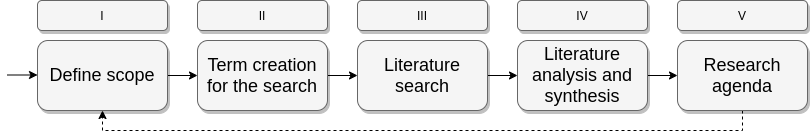
\includegraphics[width=0.9\textwidth]{literaturereview} 
    \label{figure:literaturereview} 
    \\ 
    \cite[Source: Based on][Fig. 3]{brocke2009reconstructing} 
\end{figure} 

The research is divided into a five-step process that is worked through sequentially
(Cf. Fig. \ref{figure:literaturereview}):\footcite[Cf.][pp. 2211]{brocke2009reconstructing} 

\begin{enumerate} 
    \item The first step is to define the scope of the literature review. In this case, this was done on the basis of the topics \ac{BI} and
    the mining of cryptocurrencies. In Table \ref{tbl:literaturtaxonomie} the result for the first step is shown. In
    this table, a literature taxonomy is performed according to Cooper.\footcite[Cf.][p. 2212]{brocke2009reconstructing}\footcite[Cf.][]{cooper1988organizing} 
    \item Following from this, the search terms for the literature search are formed. This step is continuously adapted depending on
    the results. Abbreviations as well as German and English terms are searched for. The used 
    search queries are listed in Table \ref{tbl:suchprozessergebnis}.\footcite[Cf.][pp. 2211]{brocke2009reconstructing} 
    \item In this step, the actual literature is searched. The search platforms used are Google
    Scholar\footnote{https://scholar.google.com}, EBSCO\footnote{https://www.ebsco.com}, Wiso\footnote{https://www.wiso-net.de}, 
    SpringerLink\footnote{https://link.springer.com}, and IEEExplore\footnote{https://ieeexplore.ieee.org}. It is ensured that,
    whenever possible, these peer-reviewed publication have appeared in scientific journals. 
    Books and online sources are also used to some extent. However, these are not used as a basis for the central
    argumentation of the paper, as these books cannot be considered scientific literature. The result of the
    search can be found in Table \ref{tbl:suchprozessergebnis}. 
    \item Next, the literature is analyzed and structured. For this purpose, subject areas are defined, to which the found literature is assigned
    to. The result of this can be found in Table \ref{tbl:konzeptmatrix}.\footcite[Cf.][p. 2214]{brocke2009reconstructing}\footcite[Cf.][]{webster2002analyzing}  
    \item The final step is to develop the research agenda based on the research gap. In this thesis, this is the application of
    \ac{BI} in the field of cryptocurrency mining. There are numerous publications on the optimization of mining
    processes.\footcite[Cf.][]{han2019demystifying}\footcite[Cf.][]{courtois2014optimizing} In addition, there are publications in the
    area of mining hardware as well as mining and blockchains in the cloud.\footcite[Cf.][]{taylor2017evolution}\footcite[Cf.][]{gai2020blockchain} 
    Furthermore, research papers can be found in the area of building mining data centers. These tend to focus on the construction of
    \ac{ASIC} based data centers, which are appropriate for Bitcoin.\footcite[Cf.][]{li2019blockchain}\footcite[Cf.][]{xie2018extreme}
    The data centers under consideration operate mining exclusively through \ac{ASIC} based hardware. Accordingly, there are numerous publications on the
    cryptomining side and on the topic of mining optimization. When looking for a connection between
    cryptomining and \ac{BI}, however, the selection is much smaller. There is literature that deals with the combination of
    cryptocurrencies and \ac{BI}, but this tends to be in the area of rates and rate trends.\footcite[Cf.][]{botocs2017bitcoin}
    Nothing can be found in the area of optimizing mining infrastructures using \ac{BI}.
    On the one hand, this is due to a few large companies operating bitcoin mining that do not publish their optimizations and efficiencies
    due to fierce competition.\footcite[Cf.][]{btccom2021miner} On the other hand, the cryptocurrency hype of the
    last few years is more in the area of investing and advancing blockchain technology and less in the area of
    mining.\footcite[Cf.][]{friedlmaier2018disrupting} 
\end{enumerate}

\begin{figure}[H]
    \caption{Method profile of business informatics}
    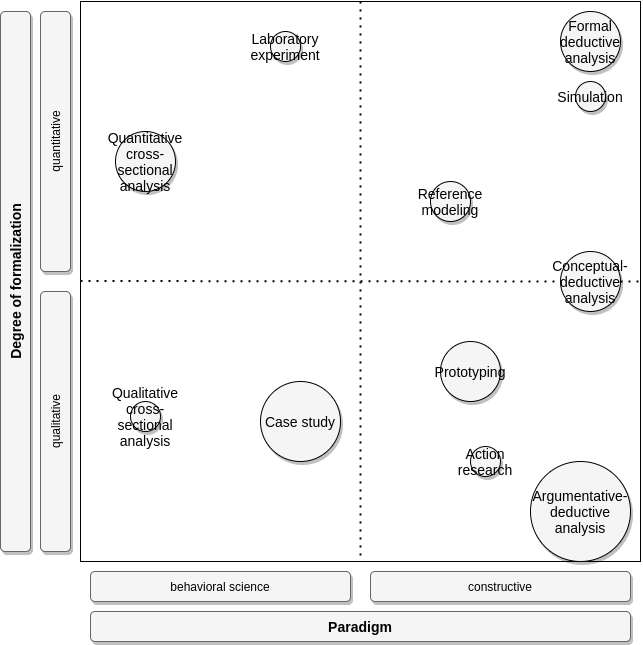
\includegraphics[width=0.7\textwidth]{methodenprofilwi}
    \label{figure:methodenprofilwi}
    \\
    \cite[Source: Based on][Fig. 3]{wilde2007forschungsmethoden}
\end{figure}

For hypotheses testing, this thesis analyzes possible methodologies in information systems in general, as well as in the field
of BI in particular.\footcite[Cf.][]{wilde2007forschungsmethoden}\footcite[Cf.][]{wilde2006methodenspektrum}\footcite[Cf.][]{jourdan2008business} 
It can be noted that both argumentative-deductive analysis and case study occupy the first two places in terms of
use.\footcite[Cf.][Fig. 2]{wilde2007forschungsmethoden} Also, the majority of publications in the field of
\ac{BI} use qualitative methods.

To be able to test the hypotheses, the following qualitative methodologies are used:

\begin{itemize}
    \item \textbf{Argumentative-deductive analysis: }This is a construction science method that is built primarily on the
    application of a logical chain of reasoning.\footcite[Cf.][Tbl. 1]{wilde2007forschungsmethoden} This is discussed in Chapter
    \ref{toc:ansatzmoeglichkeitenfuerbusinessintelligence} and is based on the foundations of the previous two chapters.
    An argumentative-deductive analysis is used to conduct the first test of the hypotheses. 
    \item \textbf{Case study: }In Chapter \ref{toc:planungeinesbiprozessesfuereinminingrechenzentrum} a case study is designed based on the theoretical
    results. This will be qualitative in nature and will represent a further test of the hypotheses. In
    difference to the argumentative-deductive analysis, the case study will test the hypotheses in a real environment.
    Therefore, a case study does not belong to the construction science methods, but to the behavioral science methods
    (Cf. Fig. \ref{figure:methodenprofilwi}). In designing the case study, we will follow the publication of Göthlich\footcite[Cf.][]{gothlich2003fallstudien}
    The stakeholder analysis is based on the publication of Simmers\footcite[Cf.][]{simmers2004stakeholder}
    The analysis of an introduction is primarily reviewed through the texts of Loshin and
    Boyer et al..\footcite[Cf.][]{loshin2012business}\footcite[Cf.][]{boyer2010business}
\end{itemize} 

By testing the hypotheses using two independent methodologies, an attempt is made to ensure that the hypotheses are analyzed from different points of view
and thus, the result of this thesis is solid.

\newpage
\section{Business Intelligence Basics} \label{toc:grundlagenbusinessintelligence}

This chapter lays the foundations for understanding \ac{BI}. Consequently, the reader should be able to understand the
\ac{BI} process in order to understand the explanations in later parts of the thesis. In order to achieve this,
the \ac{BI} process itself is explained in Chapter \ref{toc:prozess}. The following subchapters will focus on the
strategic added value of \ac{BI} and to what extent this can be measured. This becomes important for the last part of the thesis,
to understand why a project like this might be worthwhile. Ultimately, Chapter \ref{toc:einfuehrungsstrategien}
clarifies which prerequisites must be met from the operational side in order for an introduction of BI to be successful.

The term \ac{BI} originated in the 1990s and was first coined by Howard Dressner, an analyst with the Gartner Group.\footcite[Cf.][p. 96]{watson2007current}
Prior to this time, systems like \ac{DSS} and \ac{EIS} were already in place to help management
to make decisions.\footcite[Cf.][p. 1]{foley2010business}\footcite[Cf.][p. 19]{niu2009cognition}
Since then, these static systems have evolved into dynamic systems, which fall under the term \ac{BI}\footcite[Cf.][p. 26]{yeoh2010critical}
There are many different definitions for \ac{BI}, each of which have subtle differences.\footcite[Cf.][p. 114]{muntean2013agile}
A general and prominent definition is provided by Eric Foley in his paper
"What is Business Intelligence?": "Business intelligence (BI) is a combination of processes, policies, culture, and
technologies for gathering, manipulating, storing, and analyzing data collected from internal and external sources, in order to
to communicate information, create knowledge, and inform decision making. BI helps report business performance, uncover new
business opportunities, and make better business decisions regarding competitors, suppliers, customers, financial issues,
strategic issues, products and services."\footcite[][p. 4]{foley2010business} It means that \ac{BI} is an environment
in which data is collected to generate knowledge and decision support. It also provides the ability to determine
business and process inadequacies and to identify and analyze new business areas.
The possibility to carry out internal optimizations with the help of \ac{BI} is the central
reason why \ac{BI} is considered for testing the hypotheses of this thesis.

\subsection{The Business Intelligence Process} \label{toc:prozess}

In order to realize a \ac{BI} process, a multitude of logical steps are needed, which together are seen as a process.\footcite[Cf.][p. 3]{foley2010business}
Figure \ref{figure:biprocessoverview} shows the basic structure of a \ac{BI} process.
Here, the first steps are more technical in nature. During the process this changes into steps
which are more characterized by business perspectives. Consequently, knowledge is
built out of data.\footcite[Cf.][p. 13]{kasemsap2016fundamentals}

\begin{figure}[H]
    \caption{The Business Intelligence Process}
    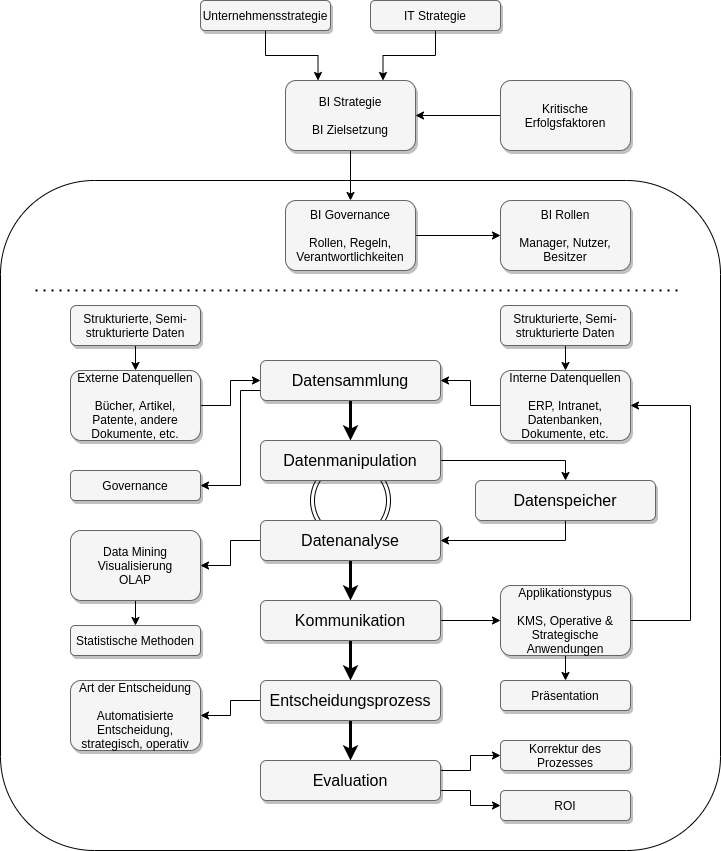
\includegraphics[width=0.7\textwidth]{biprocessoverview}
    \label{figure:biprocessoverview}
    \\
    \cite[Source: Based on][Fig. 2]{foley2010business}
\end{figure}

A \ac{BI} process breaks down into six main activities:\footcite[Cf.][Fig. 2]{foley2010business}
\begin{itemize}
    \item \textbf{Data collection: }At the beginning all data is collected. This step is needed to execute the following
    process sections. Both internal and external data sources can be used. It does not have to be
    necessarily structured data. In principle, it can also be semi-structured and unstructured data.\footcite[Cf.][p. 465]{ranjan2008business}\footcite[Cf.][p. 3]{hartmann2016capturing}
    \item \textbf{Manipulation of data: }In this step, the collected data is structured in a way that
    they can be stored in a \ac{DW}.\footcite[Cf.][p. 463]{ranjan2008business} The goal here is to have the most
    efficient data processing that takes into account the needs of the stakeholders and the users of this data.
    At the end of this step, the data is stored in a "Data Storage" (Cf. Fig. \ref{figure:biprocessoverview}).
    This is either a data warehouse or a data mart. The first two steps of the \ac{BI} process are therefore nothing else than a
    pipeline in which the data is queried, structured and stored in a \ac{DW}.\footcite[Cf.][p. 466]{ranjan2008business}
    A system like this can can be realized for example by "Apache Hadoop" and
    "Spark".\footcite[Cf.][p. 65]{rahman2015big}
    \item \textbf{Analysis of the data: }The following step is an analysis of data that can be found in a data warehouse or similar
    system.\footcite[Cf.][p. 16]{kasemsap2016fundamentals}This can be achieved by a wide variety of systems
    and is very much tailored to the objective of the process.\footcite[Cf.][p. 21]{niu2009cognition} Therefore, it is important
    that the requirements of the stakeholders are accurately implemented, so that no false analysis and results are presented and in the worst case,
    lead to completely wrong decisions. In this step, among other things, \ac{OLAP}
    systems are used, which allow multidimensional comparisons and analyses of the data.\footcite[Cf.][pp. 107]{hovcevar2010assessing}
    Other systems from the fields of machine learning and data mining are also used.\footcite[Cf.][p. 11]{foley2010business}\footcite[Cf.][p. 80]{yeoh2008managing}
    Additionally, the
    execution of simulations (for example, Monte Carlo simulations) is possible in this step. Finally, at
    the result of the analyses and calculations, the management is provided with knowledge, which has an advantage over competitors, especially with respect to
    decision-making processes.\footcite[Cf.][p. 94]{hovcevar2010assessing}
    \item \textbf{Communication and Access: }Doing data analysis leads to extraction of knowledge from data.
    Making this knowledge accessible is the task of this step. The aim here is to ensure that the knowledge
    is made accessible to the right stakeholders via the right medium.\footcite[Cf.][p. 11]{foley2010business} These
    forms of media can be dashboards, reports, scorecards and other methodologies.\footcite[Cf.][pp. 21]{niu2009cognition} At the end
    of this step, the knowledge is accessible to stakeholders ensuring the next step.
    \item \textbf{Decision Process: }In this step, the actual decision is made by the relevant stakeholder.\footcite[Cf.][p. 12]{foley2010business}
    In this process, the processed data are made available to support the
    decisions. This allows them to transparently base their decisions on the data collected.\footcite[Cf.][p. 13]{kasemsap2016fundamentals}
    \item \textbf{Evaluation: }The final step is to evaluate whether the \ac{BI} system brings the desired improvements or benefits.
    On the one hand, it can be shown that the system is financially worthwhile and contributes to the success of the company.\footcite[Cf.][p. 12]{foley2010business}
    On the other hand, corrective measures can also be introduced in this step,
    if the \ac{BI} process did not bring the desired success.\footcite[Cf.][p. 12]{foley2010business}
    This approach gives the entire \ac{BI} process an agile and cyclical character.
\end{itemize}

As can be seen in Figure \ref{figure:biprocessoverview}, there are other factors that contribute to a functioning
\ac{BI} process. First and foremost, these include the strategy and goal definition of a \ac{BI} project. These are decisively
influenced by the \ac{CSF}. In Chapter \ref{toc:einfuehrungsstrategien}, the factors are analyzed in more detail, as they have a
significant influence on a successful implementation. In addition, there is the issue of "IT governance".
In the case of \ac{BI}, this refers to the set of all guidelines and the bodies responsible for ensuring that the
areas of the project are clearly regulated.\footcite[Cf.][p. 8]{foley2010business} Finally, with the
the introduction of this governance the \ac{ROI} of the \ac{BI} Project can be supported.\footcite[Cf.][p. 8]{foley2010business}

\subsection{Added value for businesses} \label{toc:strategischermehrwert}

In IT projects, it is usually difficult to estimate the total added value for a company, which can be defined primarily by the
\ac{ROI}.\footcite[Cf.][p. 97]{hovcevar2010assessing} This is due to the division of added value
into financial factors, which are comparatively easy to name, and into non-financial factors, which are indirectly measurable
and therefore can only be estimated.\footcite[Cf.][p. 93]{hovcevar2010assessing} This also applies to \ac{BI} processes. Since a BI process' central advantage
is in supporting an often complex management decision-making process, the
financial impact may only be estimated.\footcite[Cf.][pp. 94]{hovcevar2010assessing} Figure
\ref{figure:mehrwertbi} lists added values that an \ac{BI} process can have for an organization. These are ranked in descending order
by the difficulty of measuring the financial value added.

\begin{figure}[H]
    \caption{Added value of Business Intelligence}
    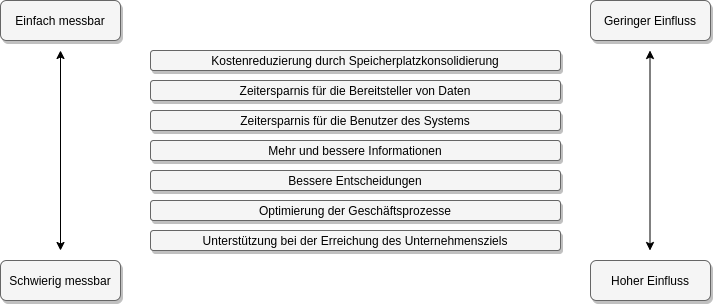
\includegraphics[width=0.85\textwidth]{mehrwertbi}
    \label{figure:mehrwertbi}
    \\
    \cite[Source: Based on][Fig. 2]{watson2007current}
\end{figure}

According to Figure \ref{figure:mehrwertbi}, the added value of a BI process can be divided into the following areas:\footcite[Cf.][Fig. 2]{watson2007current}

\begin{itemize}
    \item By introducing a data warehouse or a data mart, company-relevant data is stored in one place for analysis.
    Costs for a multitude of heterogeneous storage locations can be reduced. The availability
    of the data is improved. As a result, a reduction in costs is possible through a uniform system of data storage.\footcite[Cf.][p. 105]{azma2012business}
    \item Due to automated data procurement for the data warehouse and fast availability through \ac{OLAP} systems,
    time saving in the process of data procurement and provision can also be measured.\footcite[Cf.][p. 51]{horakova2013business}
    This can be translated into a financial measure and considered in costs analysis.
    \item Since business-relevant data is stored in one place, making it quickly available to users,
    time saving is measurable for the stakeholders of the system.\footcite[Cf.][p. 97]{williams2003business} As with the
    last point, this can also be added to the analysis.
    \item As one of the results of the BI process, information and knowledge are available more quickly. The quality of the
    information is higher than before because the information is based on larger amounts of data, more data sources and better analysis
    parameters\footcite[Cf.][p. 51]{horakova2013business}. Parameters as information quality are factors
    that can only enter into a financial analysis by estimation.\footcite[Cf.][p. 51]{horakova2013business}
    \item As a consequence of the better information situation, management is now in a position to make better
    decisions. As described at the beginning, this sort of decision can be measured poorly in financial terms due to the high complexity and the large impact of the decision.\footcite[Cf.][p. 51]{horakova2013business}
    In addition, the opportunity costs are difficult to measure.\footcite[Cf.][p. 99]{hovcevar2010assessing}
    \item Business processes can be optimized using \ac{BI}. This is due to the better information situation and
    thus the possibility to identify inadequacies. The advantage obtained in this way is
    difficult to assess, as it is not possible to predict in advance to what extent process optimization will be necessary and what the financial impact will be.\footcite[Cf.][p. 2]{williams2003business}
    \item One of the foundations for the introduction of \ac{BI} is a clear business objective (see Chapter \ref{toc:einfuehrungsstrategien}).
    \ac{BI} can help to achieve this faster and better. However, since there are many more factors than only one \ac{BI} process that contribute to the achievement
    of the business goal, it is difficult to identify the rightful share and to include it in the
    analysis of the added value.\footcite[Cf.][p. 51]{horakova2013business}
\end{itemize}

In contrast to the added value, the costs for a \ac{BI} project can be estimated quite easily by considering the infrastructure,
software, and the project team.\footcite[Cf.][p. 98]{hovcevar2010assessing} The cost savings
and revenue generated by a \ac{BI} process must exceed expenses for a \ac{ROI} to be measurable.\footcite[Cf.][p. 8]{williams2003business}
Only if this is possible, an enterprise-wide added value of the project can be
identified and thus its meaningfulness can be demonstrated to the management. In summary it
can be stated that the main added value of BI can be defined as follows: "the business value of BI lies in
its effective use within management processes and/or operational processes that drive revenue or reduce
costs."\footcite[][p. 7]{williams2003business}

\subsection{Prerequisites for a successful introduction} \label{toc:einfuehrungsstrategien}

The prerequisites necessary for successful implementation are described as critical success factors.

\begin{figure}[H]
    \caption{Prerequisites for a successful BI implementation}
    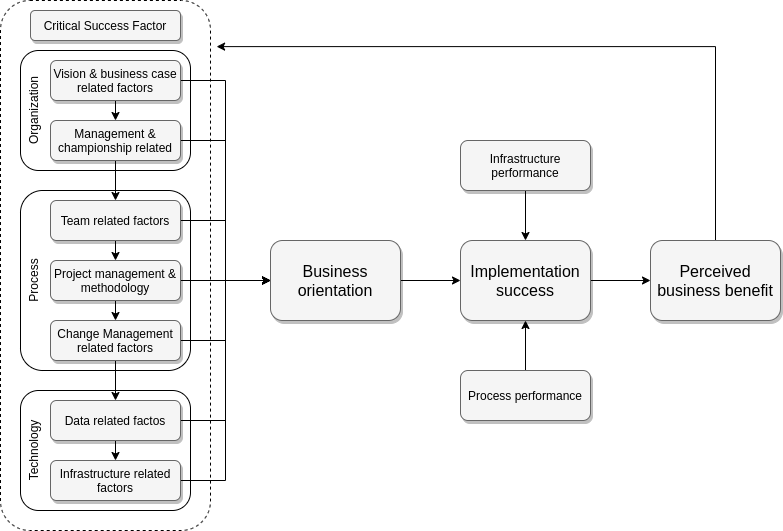
\includegraphics[width=0.85\textwidth]{bisuccessfactors}
    \label{figure:bisuccessfactors}
    \\
    \cite[Source: Based on][Fig. 1]{yeoh2010critical}
\end{figure}

In Figure \ref{figure:bisuccessfactors}, these success factors are divided into three different dimensions and thus different
viewpoints.\footcite[Cf.][pp. 26]{yeoh2010critical} Using these dimensions, it is later possible to perform a
stakeholder analysis for a \ac{BI} process. The three different perspectives can be defined as follows:

\begin{itemize}
    \item \textbf{Organizational View: }This dimension is based on a view from the direction of the organization.
    There are two points that make the success of a \ac{BI} process possible. The first point requires that the project
    receives clear support from management. This ensures that the project has sufficient financial and human resources.\footcite[Cf.][p. 98]{watson2007current}
    A project sponsor on the part of the management is recommended.\footcite[Cf.][pp. 87]{yeoh2008managing}
    The second point is that the project must have a clear objective and vision.\footcite[Cf.][pp. 87]{yeoh2008managing}\footcite[Cf.][p. 50]{villamarin2017key}
    A company that wants to to implement a process like this should have a clear vision.
    Based on this, it is possible to formulate the project vision and ultimately define a clear
    objective for the project.\footcite[Cf.][pp. 87]{yeoh2008managing}
    \item \textbf{Process View: }This view looks at the actual processes and requirements at the project level.
    First and foremost, there is a project management team that is capable of managing the project. This project manager should have the
    technical, organizational, and process perspectives.\footcite[Cf.][p. 27]{yeoh2010critical}He must be as familiar with the
    processes in the company as with the characteristics of the technical systems used to solve the problem.\footcite[Cf.][pp. 88]{yeoh2008managing}
    In addition, a well-balanced team composition is very important.\footcite[Cf.][pp. 87]{yeoh2008managing}
    Since the implementation of BI processes is typically of an
    interdisciplinary nature, the team should consist of both specialists in technology and specialists in
    data analysis, data presentation, and business processes.\footcite[Cf.][Fig. 7]{muntean2013agile} Last but not least.
    a flexible and agile development approach is recommended, since \ac{BI} systems in particular should react quickly to changing requirements.
    Only through this flexibility is it possible to react quickly if something needs to be changed, improved
    or should be updated. One methodology to achieve this is
    Scrum.\footcite[Cf.][p. 164]{isik2011business}\footcite[Cf.][p. 3817]{knabke2013understanding}
    \item \textbf{Technological view: }Finally, the technological view is important. This is divided into two
    subject areas: On the one hand, there are the success factors that deal with the data\footcite[Cf.][Fig. 1]{yeoh2010critical}
    These factors primarily describe the nature of the data used.
    Two requirements are placed on the data: The data should be of both high quality and high
    integrity.\footcite[Cf.][p. 163]{isik2011business} Both could lead to distorted results,
    which could lead to an unusable BI system. On the other hand, there are factors that affect the infrastructural side.\footcite[Cf.][Fig. 1]{yeoh2010critical}
    Above all, the underlying infrastructure should be flexible and
    scalable. It must be able to respond to changing demands on the project.\footcite[Cf.][pp. 89]{yeoh2008managing}
\end{itemize}

On the basis of these critical success factors, it is possible to check during project planning whether the most important
prerequisites for a project implementation are given. Later in this work, an analysis like this will be carried out concretely.
\newpage
\section{Cryptomining basics} \label{toc:grundlagenkryptomining}

\acused{SHA}

This chapter lays the foundations for understanding the term "cryptomining". After this part, the reader should
have a picture of what mining is and why, in the blockchain domain, mining is a fundamental process. Furthermore
he should be able to understand the basic structure of an enterprise data center that is exclusively mining.
To achieve this, the first step in chapter \ref{toc:kryptowaehrungenundblockchain} is to give a brief
introduction to the blockchain and its basic structure. There, it is established why the principle of
mining was introduced and what it is used for. In the chapter \ref{toc:miningundkonsensalgorithmen}, the process of
of the mining is dealt with. The basic functioning and necessity of mining is shown. After
these basics are laid, the operation of a mining data center is described. The understanding of
data centers that specialize in mining is important for the rest of the paper, as they are to be optimized from a financial perspective.
For this purpose, the basic structure of such a data center of the Genesis Group is exemplarily
described. It is shown which \acp{KPI} of these data centers are important. These are used to optimize the
data centers to be able to optimize them financially. All this is discussed in chapter \ref{toc:miningrechenzentren}. Following
this knowledge is then used to identify possible starting points for a business intelligence system
and to model an exemplary process at the end of the thesis.

\subsection{Basic technologies} \label{toc:technologie}

The concept of blockchain was first described in 2008 in a whitepaper using the example of Bitcoin,
published by the pseudonym Satoshi Nakamoto.\footcite[Cf.][]{nakamoto2008bitcoin} Many companies and start-ups in
a wide variety of industries are looking at blockchain-based
systems, such as in the financial industry, in the information sector, but also in the health care and
transport sectors.\footcite[Cf.][Chap. 4.1]{friedlmaier2018disrupting} Another branch that has emerged through the introduction of
cryptocurrencies are companies that specialize in mining cryptocurrencies. To understand the
technical basis for this business case, the following two subsections describe what
a blockchain is and what characteristics make mining necessary. How mining is technologically implemented and why
it provides a way to make money is described in chapter \ref{toc:miningundkonsensalgorithmen}.

\subsubsection{Definition of Blockchain} \label{toc:kryptowaehrungenundblockchain}

A blockchain, as the name translates, is a chain of blocks. Through the use of cryptographic
processes, data on a blockchain is subsequently stored immutably, which can make this technology attractive for many
applications.\footcite[Cf.][p. 1]{friedlmaier2018disrupting} The atomic unit of a blockchain
is a single block. In the case of Bitcoin, this consists of two different parts: a list of transactions
and the so-called "block header", which contains the most important meta-information and properties of the block.\footcite[Cf.][p. 48]{bhaskar2015bitcoin}\footcite[Cf.][p. 4]{nakamoto2008bitcoin}

\begin{figure}[H]
    \caption{Structure of a single block}
    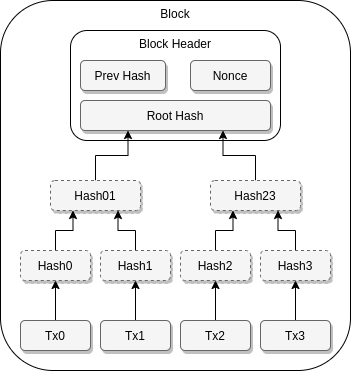
\includegraphics[width=0.4\textwidth]{blockstructure}
    \label{figure:blockstructure}
    \\
    \cite[Source: Based on][p. 4]{nakamoto2008bitcoin}
\end{figure}

The following is a list of the elementary parameters that can be found in a block header
(Cf. Fig. \ref{figure:blockstructure}):

\begin{itemize}
    \item \textbf{Previous block hash: }Because the blocks are arranged into a logical chain, there must be some way
    to identify the order in which the blocks are written. This is achieved similar to a
    chained list by calculating a hash from the block header of the previous block by applying the \ac{SHA}256
    hash function and entering it into the field "Previous block hash".\footcite[Cf.][p. 4]{nakamoto2008bitcoin} This achieves,
    that the sequence of blocks in the blockchain is well-defined back to the first block ("Genesis Block")\footcite[Cf.][Fig. 3.2]{bhaskar2015bitcoin}
    and is traceable (Cf. Fig. \ref{figure:blockchainstructure}).
    Subsequent modification of a block will cause the chain to break, as this will change the hash value of the
    tampered block.
    \item \textbf{Merkle Root: }This field is used to enter the result of the Merkle tree, which is calculated from all transactions.\footcite[Cf.][p. 4]{nakamoto2008bitcoin}
    This is also a hash value. A hash value is formed from
    each individual transaction and merged into a hash value via a binary tree. This value is called
    "Merkle Root" (cf. \ref{figure:blockstructure}). This allows the integrity of each transaction
    which is located in this block. A subsequent change is no longer possible, because in this case,
    the hash value of the Merkle root in the block header and thus the resulting hash of the block header would change.
    Consequently, the chain would break in this case and the blockchain would be destroyed.
    \item \textbf{Nonce: }This is a random number used to generate a hash of the block header,
    which is subject to certain constraints.\footcite[Cf.][p. 745]{mukhopadhyay2016brief}\footcite[Cf.][p. 136]{courtois2014optimizing}
    Guessing and verifying this value is called mining.\footcite[Cf.][pp. 50]{bhaskar2015bitcoin}\footcite[Cf.][p. 24]{han2019demystifying}
    How this value is found and what rules it must obey is described in chapter \ref{toc:miningundkonsensalgorithmen}
    described.
\end{itemize}

\begin{figure}[H]
    \caption{Schematic structure of the blockchain}
    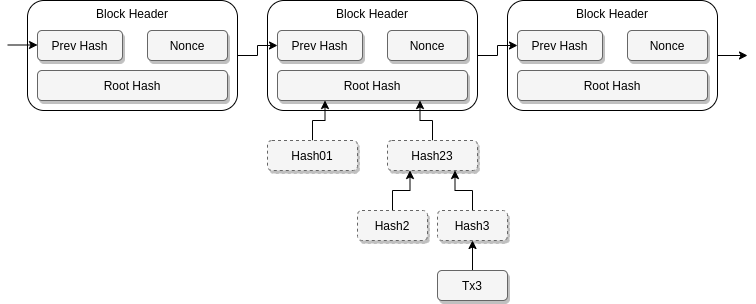
\includegraphics[width=0.8\textwidth]{blockchainstructure}
    \label{figure:blockchainstructure}
    \\
    \cite[Source: Based on][p. 5]{nakamoto2008bitcoin}
\end{figure}

The rest of the block, which in the case of Bitcoin is limited to the size of 1MB, is filled with the corresponding
transactions that have been used to calculate the Merkle root.\footcite[Cf.][p. 746]{mukhopadhyay2016brief}
In general, any data can be stored on a blockchain. There are no restrictions that
it must be transaction data of a currency.

Now there are still two ways to change or delete the data on a blockchain. One case
is the manual deletion of the blockchain. To prevent this, a blockchain is stored in a decentralized manner on many
devices.\footcite[Cf.][p. 46]{bhaskar2015bitcoin} Each of these devices contains a current and correct copy
of the blockchain with all of its data. Such a device is called a "node". Any person in the world can inpect the blockchain, in the case of
Bitcoin, because the data of the Bitcoin Blockchain is publicly available and therefore it is a so-called "permissionless blockchain".\footcite[Cf.][p. 132]{courtois2014optimizing}
If a participant deletes his node or the node is simply
deletes its node or it simply fails, the blockchain is still available and not deleted due to the decentralized replication.

The other case is the modification of a block and a subsequent complete recalculation of all hash values of this blockchain,
which would again result in a new correct blockchain. However, this would contain falsified data.
To prevent this, mining has been introduced, which is nothing more than a guessing game to find the
correct value of the "nonce" described above. This principle is called \ac{PoW} and will be described in detail in the next chapter.\footcite[Cf.][p. 3]{nakamoto2008bitcoin}

In summary, it can be stated that a blockchain is extremely secure against falsification and deletion of data due to its
strong use of cryptographic processes and its decentralization.
The first obvious use case was the application of the blockchain to introduce a digital and decentralized currency, as Satoshi
Satoshi Nakamoto also proposed in his white paper.\footcite[Cf.][]{nakamoto2008bitcoin}

\subsubsection{Definition of mining} \label{toc:miningundkonsensalgorithmen}

Building on the last chapter, this chapter deals with the functioning of mining and the underlying consensus algorithms.
This is important for the remainder of the thesis, since it explains the basic structure of mining
and also during the mining process, important parameters such as the "difficulty" play a role in the overall financial assessment of a mining project,
which contribute to an overall financial assessment of a data center.

Based on the problem that the Bitcoin blockchain consists of a decentralized peer-to-peer network, it is necessary to
be asked how a consensus is generated between the participants and how it is ensured
that fraudulent intentions are prevented. The question becomes how all participants together can reach a valid
consensus and thus make the blockchain trustworthy.\footcite[Cf.][Fig. 3]{derks2018chaining}
To answer these questions, we will look at possible consensus algorithms and explore the principle of
of mining is explained on the basis of the \ac{PoW} consensus.

The first consensus algorithm was described in Satoshi Nakamoto's Bitcoin whitepaper and is called
"Proof-of-Work".\footcite[Cf.][p. 3]{nakamoto2008bitcoin} Since it is not optimal in terms of energy consumption, other algorithms have been developed,
that are much more energy efficient.\footcite[Cf.][]{dwcom2021bitcoin} The best known example is \ac{PoS} or also the use of the
"byzantine fault tolerance", which is also known as the "problem of the Byzantine generals" across the blockchain
industry.\footcite[Cf.][p. 2]{friedlmaier2018disrupting}\footcite[Cf.][p. 746]{mukhopadhyay2016brief}
However, since large computational resources are required only for proof-of-work, the following discussion will focus on this algorithm
using the example of Bitcoin.

The process of mining through proof-of-work can be divided into the following steps:\footcite[Cf.][p. 3]{nakamoto2008bitcoin}\footcite[Cf.][p. 51]{li2019blockchain}

\begin{enumerate}
    \item New transactions are sent to all nodes in the network. These are stored in the so-called "mempool",
    a cache of transactions that have not yet been confirmed, and held for the mining process.
    \item Transactions are packaged into a block by the nodes. The transactions with the highest fees,
    which can be freely chosen by the client, are preferentially merged from the mempool into a block.\footcite[Cf.][p. 53]{bhaskar2015bitcoin}
    The sum of the transaction fees of the block is attributed to the miner
    once he finds a valid block.\footcite[Cf.][p. 4]{nakamoto2008bitcoin}
    \item The mining hardware computes a valid proof-of-work for that block, which the nodes provide to the network.
    This is the actual computationally intensive process. Basically, this process is nothing more
    other than a brute-forcing of hash values.\footcite[Cf.][p. 747]{mukhopadhyay2016brief} Only in this way
    it is possible to compute a correct target hash value, since hash functions are surjective. The so called
    "difficulty" is used to determine how many zeros the resulting hash should start with.\footcite[Cf.][p. 57]{bhaskar2015bitcoin}
    In order to find a suitable hash, the nonce is varied and
    for each value of the nonce, the hash value of the block is computed and verified. If it meets the requirements, which are
    specified by the difficulty, a valid \ac{PoW} has been found. On average, this process should take about ten minutes.\footcite[Cf.][p. 748]{mukhopadhyay2016brief}
    Therefore, the relevant performance metric of the mining hardware is called the
    hashrate.\footcite[Cf.][p. 49]{bhaskar2015bitcoin} This describes how many hash values a device can compute in one second.
    If the overall hashrate in the Bitcoin network increases, so does the
    probability that a valid proof-of-work can be found in less than ten minutes. Therefore, the
    Difficulty is adjusted every 2,016 blocks, so that if the overall hashrate of the network is higher, the variation
    of the starting zeros makes it easier or more difficult to find a valid proof-of-work (Cf.
    Fig. \ref{figure:evolutiondifficulty}).\footcite[Cf.][p. 57]{bhaskar2015bitcoin} Since the creation of the blocks
    takes a lot of computational work, individual fraudsters now have no ability to manipulate the blockchain,
    as long as the majority of participants in mining are honest. 
    \item When a proof-of-work is found, it is sent to all nodes in the Bitcoin network.\footcite[Cf.][pp. 3]{nakamoto2008bitcoin}
    For this purpose, the node connected to the mining hardware forms a
    valid nonce with all the other information and sends it to all nodes in the Bitcoin network.
    \item This block is now verified by the remaining nodes. The verification is successful as soon as the majority of
    nodes accept the block and the construction of a new block is started, using the hash value of the found block as the
    block is used as the previous hash for the new block.\footcite[Cf.][pp. 3]{nakamoto2008bitcoin}
    The operator of the mining hardware receives as a reward the sum of all transaction fees of the block and
    a fixed amount, which is currently 6.25 \ac{BTC} per block.\footcite[Cf.][p. 4]{nakamoto2008bitcoin}\footcite[Cf.][]{btcecho2021halving}\footcite[Cf.][p. 59]{taylor2017evolution}
    The 6.25 \ac{BTC} is called a "block reward." This was initially 50 \ac{BTC} and is reduced by half every 210,000 blocks.\footcite[Cf.][p. 58]{taylor2017evolution}
    This will provide the Bitcoin network with new and
    fresh currency. Subsequently, the process of mining starts all over again.
\end{enumerate}

\begin{figure}[H]
    \caption{Development of the Difficulty of Bitcoin depending on the used hardware and grid size}
    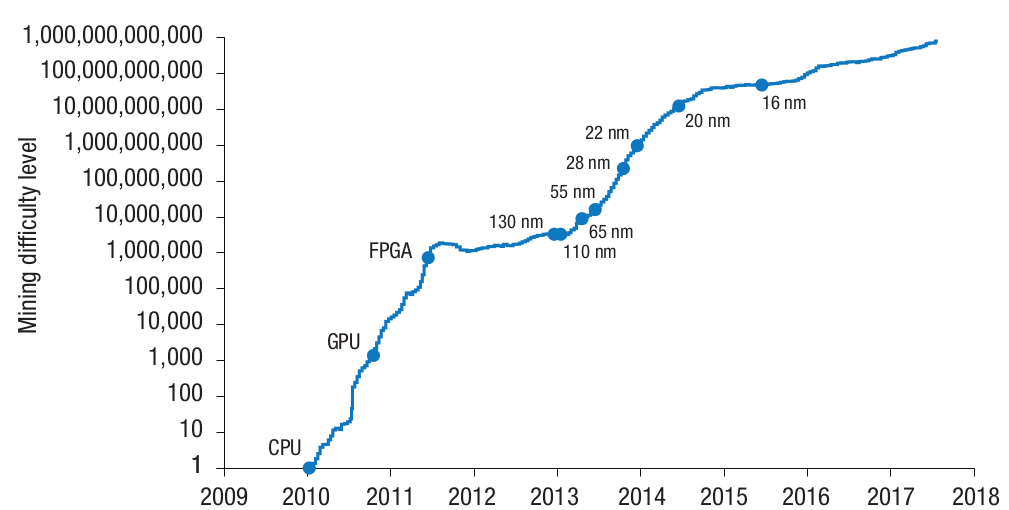
\includegraphics[width=0.8\textwidth]{evolutiondifficulty}
    \label{figure:evolutiondifficulty}
    \\
    \cite[Source: ][Fig. 1b]{taylor2017evolution}
\end{figure}

In principle, the higher your own share of the total hashrate of the network, the higher the probability of successfully finding a block first.
For this reason, operators of mining hardware try to give as much
performance as possible to the network in order to obtain the highest possible payouts. The operation
takes place in relation to the cost of such infrastructure, which is discussed in chap.
\ref{toc:kennzahlenundeinflussfaktoren} in more detail.

Basically, anyone can participate in mining. There are currently three models of how mining can be
done:\footcite[Cf.][p. 53, pp. 57]{bhaskar2015bitcoin}

\begin{itemize}
    \item \textbf{Solo Mining: }This describes the classic method in which participants use their own hardware
    and perform mining. They receive the entire proceeds of a block after a successful proof-of-work.
    \item \textbf{Mining Pools: }In mining pools, the hashrate of many miners is pooled. By pooling the hashrate,
    the probability of finding a valid block is increased. The payout in this
    not the total yield of the block, but rather the percentage of the output that is made available to the mining pool.
    Due to the participation, the individual yields will be lower but more evenly
    turn out. This avoids the risk of not finding a valid proof-of-work for a long time as a solo miner.
    (see Fig. \ref{figure:valuechaindatacenter}).\footcite[Cf.][pp. 58]{bhaskar2015bitcoin}\footcite[Cf.][p. 327]{derks2018chaining}
    \textbf{Mining Contracts: }The third option is to rent mining hardware or purchase a
    hashrate. \footcite[Cf.][pp. 58]{bhaskar2015bitcoin}The proceeds from mining are transferred to the person after deducting the
    contract fees. Consequently, the person does not need to operate his own hardware and can leave this to professional
    companies that can do this much more efficiently than private individuals. Such a product is offered by the
    Genesis Group.
\end{itemize}

\subsection{Mining data centers} \label{toc:miningrechenzentren}

Mining Bitcoins has changed a lot since its introduction in 2009. At that time, hashes were started to be calculated on
normal \acp{CPU}.\footcite[Cf.][pp. 97]{xie2018extreme}\footcite[Cf.][p. 62]{taylor2017evolution}
As explained in chapter \ref{toc:miningundkonsensalgorithmen}, the likelihood of finding a block successfully using proof-of-work
increases with the proportional hashrate to the total network hashrate.
Accordingly, mining hardware operators aim to increase efficiency by reducing the cost per
computed hash. Due to this endeavor, the second generation of mining hardware based on
\acp{GPU} has been developed.\footcite[Cf.][p. 98]{xie2018extreme}\footcite[Cf.][p. 62]{taylor2017evolution}
Due to the evolution of Bitcoin's network hashrate, third-generation hardware based on the
\acp{FPGA} basis.\footcite[Cf.][p. 98]{xie2018extreme}\footcite[Cf.][pp. 62]{taylor2017evolution}
The fourth-generation hardware type is still in use today and is based on
\acp{ASIC}.\footcite[Cf.][pp. 98]{xie2018extreme}\footcite[Cf.][p. 15]{gai2020blockchain} These devices are
specialized by hardware layout to compute hashes highly efficient.{gai2020blockchain}
On the other hand, these chips are not able to compute other things efficiently and thus are only designed for this
specific purpose they were developed. However, there has been a drive not only for higher efficiency, but also
for scaling the mining hardware. In order to maximize the returns from mining, these two drivers have been
combined. This led to the construction of highly specialized ASIC-based data centers dedicated solely to bitcoin mining.\footcite[Cf.][p. 97]{xie2018extreme}
Several such data centers are operated by Genesis Group. These are
described below as examples and their cost and value structure analyzed.

\subsubsection{Structure and operation} \label{toc:aufbauundfunktionsweise}

This chapter describes how a data center that specializes in bitcoin mining is structured
and how it performs mining.

The central component of a mining data center is the mining hardware.\footcite[Cf.][p. 327]{derks2018chaining}
The number of devices operated in such a data center is basically limited only by external factors
such as available space and power supply. In the paper "`Extreme Datacenter Specialization for Planet-Scale.
Computing: ASIC Clouds"', it is described that the devices are usually housed in server racks.\footcite[Cf.][Fig. 5]{xie2018extreme}
This is usually not the case for mining data centers,
as most of the hardware is not built in a 19-inch form factor. Instead, matching heavy-duty racks are
are used, which are placed in rows. Many such rows make up the data center in
itself.\footcite[Cf.][]{appendix:layoutkardok}

As the mining hardware consumes a lot of power, special attention must be paid to the power supply.\footcite[Cf.][p. 327]{derks2018chaining}
The necessary electricity is purchased from external energy companies. The
substations and necessary transformer facilities are located on the outside of the data center or very close by
and ensure a stable power supply. Within the data center, high-voltage sub-distribution boards are
required to supply the individual devices. One of the current models,
the S19 Pro Miner from Bitmain, consumes an average of 3.25kW per device.\footcite[Cf.][]{s19pro2021consumption}
Assuming that there are approximately 12,000 devices in a data center, this results in total
power consumption of 39.0MW for the mining hardware.

In order for the miners to operate stably, the waste heat from the devices must be efficiently removed. For this purpose
a basic structure identical to an ordinary data center consisting of hot and cold aisles is used.
Fans transport cold air into the data center from outside. This warms up as it flows through the
mining hardware, and is carried away through the hot aisle.\footcite[Cf.][]{appendix:layoutkardok} The
electricity costs for cooling make up a significant portion of a mining data center's electricity costs.

In order for the mining hardware to communicate with the blockchain nodes, a network infrastructure is required in addition to the power supply.
This is designed in such a way that each device can communicate with the Internet and thus also with the nodes.
Due to the bandwidth requirements of the internal network, the central
components are dimensioned with a throughput of 10$\frac{Gbit}{s}$. For the peripherals, a data volume of
of 1$\frac{Gbit}{s}$.\footcite[Cf.][]{appendix:networktopology} In order to keep the bandwidth into the internet as small as possible
the mining hardware is connected to a mining proxy, which is installed on an internal server and
and connects to the Bitcoin network and the mining pool used.\footcite[Cf.][]{appendix:miningproxy}
The advantage is that only one connection is needed to an external mining pool.

Finally, control and monitoring software for the mining hardware is installed on additional internal servers.
This software controls and monitors a large number of mining devices.\footnote{https://www.genesis-mining.com/hexa}
The data obtained from the monitoring can be very
interesting for use within business intelligence processes. This evaluation is done
in chapter \ref{toc:ansatzmoeglichkeitenfuerbusinessintelligence}.

\subsubsection{Financial considerations} \label{toc:kennzahlenundeinflussfaktoren}

In diesem Teil wird nun beschrieben, welche finanziellen und nicht-finanziellen Einflussfaktoren bei einem
Rechenzentrum, das sich auf Mining spezialisiert hat, existieren. Dazu wird sich bei finanziellen Aspekten auf interne
Dokumentationen gestützt. Diese werden zusätzlich kategorisiert, ob es sich um \ac{CapEx} oder \ac{OpEx} Posten und
ob es sich um variable oder fixe Kosten handelt. Weiterhin werden Faktoren erläutert, die die Einnahmen des Rechenzentrums
optimieren können und wie die Rentabilität gemessen werden kann (\acp{KPI}). Richtung Ende werden Einflussfaktoren
gelistet, die nicht-finanzieller oder nicht-technischer Natur sind und momentan daher grundsätzlich nur in einem geringen
Detaillierungsgrad in Betracht gezogen werden können. Sprungfixe Kosten werden in diesem Teil nicht verwendet, da die
zugrundeliegenden Berechnungen und Abschätzungen diese auch nicht als Kostensorte berücksichtigen.

In this section, we will now describe the financial and non-financial factors that influence a data center that specializes in mining.
The financial aspects are based on internal documentation.
These are additionally categorized as to whether they are \ac{CapEx} or \ac{OpEx} items and
whether they are variable or fixed costs. Furthermore, factors are explained that can optimize data center revenues
and how profitability can be measured (\acp{KPI}). Towards the end, influencing factors are
listed that are non-financial or non-technical in nature and are therefore currently only considered in a low level of detail.
Leap-fixed costs are not used in this part, since the
underlying calculations and estimates do not take them into account as cost items.

In the first step, the costs of a data center are fundamentally divided into \ac{CapEx} and \ac{OpEx}\footcite[Cf.][]{appendix:capex}\footcite[Cf.][]{appendix:opex} \ac{CapEx}
describes the initial
expenditures that must be made to build a data center. \ac{OpEx} describes the kind of costs, which are permanently
during the operation. Both items are additionally subdivided into fixed or variable costs, which depend on the number of miners
that are installed on site.

\begin{figure}[H]
    \caption{Cost structure of a mining data center}
    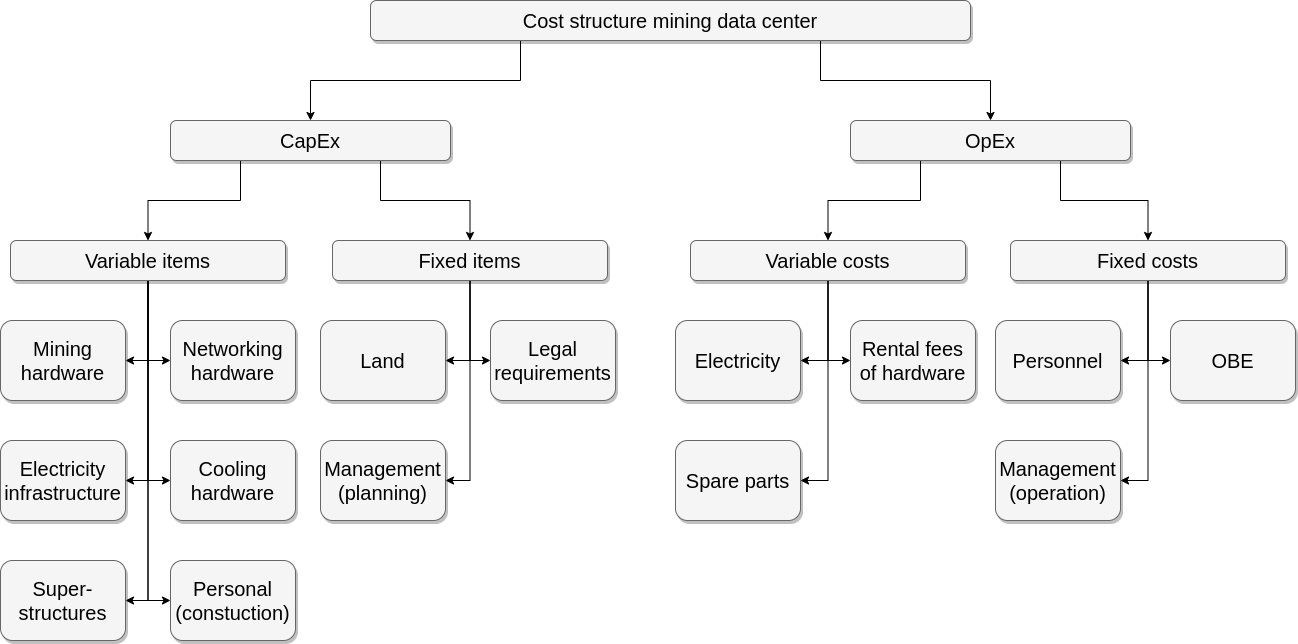
\includegraphics[width=\textwidth]{valuestructurenordics}
    \label{figure:valuestructurenordics}
\end{figure}

This division can be found in Fig. \ref{figure:valuestructurenordics}. The following items are relevant to the structure
a data center:\footcite[Cf.][]{appendix:capex}
\begin{itemize}
    \item \textbf{Mining Hardware: }This item refers to the actual special hardware that is needed for the
    Bitcoin mining (see item 2 in Fig. \ref{figure:valuechaindatacenter}). The \ac{KPI}, which measures the
    effectiveness of the device is the amount of average payouts from mining. This ranges
    for current models, such as the Antminer S19Pro, at about $0.06\ USD / \frac{TH}{s} / day$ in the worst case, means
    \ac{USD} per hashrate per day.\footcite[Cf.][]{appendix:worstcasescenario} In the most likely scenario,
    it is $0.09\ USD / \frac{TH}{s} / day$\footcite[Cf.][]{appendix:mostprobablescenario} and in the optimal scenario
    at $0.27\ USD / \frac{TH}{s} / day$.\footcite[Cf.][]{appendix:optimalscenario} The identification of the correct
    scenario is based on the Difficulty of Bitcoin mining, the total network Hashrate and the market value
    of a Bitcoin, which are additional \acp{KPI} when operating a data center. Since the market value is extremely
    volatile, it is difficult to make an accurate prediction.\footcite[Cf.][p. 325]{badertscher2017bitcoin} In addition
    this part includes the downtime and the fees for the mining pool in a lump sum
    factored in.\footcite[Cf.][]{appendix:s19proassumptions} The effectiveness of the mining hardware is
    calculated by the following equation:
    \begin{equation}
        \RM = \frac{\DP}{\THr}\cdot(1-\PF)\cdot\UT\cdot\ER
    \end{equation}
    In this formula, the daily expected payouts (\DP) per hashrate (\THr) are calculated. The result is
    corrected by uptime of the mining hardware (\UT), fees (\PF) and the exchange rate of \ac{USD} and \ac{BTC}.

    In this calculation, the electricity price is not listed directly. This value is calculated by the power consumption of the
    devices. Improvements in the firmware of these devices can be visualized with a \ac{KPI} called
    "`Reference power effiency'". This has the unit $\frac{J}{TH}$ (joules per terahash) and is strongly
    temperature dependent.\footcite[Cf.][]{s19pro2021consumption}

    The mining hardware item is variable as it is proportional to the number of miners. For a
    10MW data center, this would be approximately S19 2,987 per miner\footcite[Cf.][]{appendix:s19proassumptions} for a total price of
    of about 8,068,708 USD.\footcite[Cf.][]{appendix:capex}
    \item \textbf{Network Hardware: }In order for the mining hardware to communicate with the blockchain, network
    Hardware is required. Switches, routers and network cables fall under this item. Standardized network hardware is used
    that is cheap and available in large quantities. This item is also
    variable, as the number and length of network cabling and the number of switches increases with the number of mining hardware.
    of switches increases.\footcite[Cf.][]{appendix:capex} While the number of routers remains constant, it represents such a
    small proportion of this item that it can be considered variable. For a 10MW data center
    the cost of this item is approximately 69,060 USD.\footcite[Cf.][]{appendix:capex}
    \item \textbf{infrastructure electricity: }For the operation of the mining hardware, one item when setting up a
    of a mining data center is the power supply. This item mainly refers to the cabling within the data center.
    The grid connection and the heavy current transformers are included in other items in the invoice.
    Since the number of cables and distributors within a data center increases as the number of mining
    equipment increases, this is a variable item in the construction.\footcite[Cf.][]{appendix:capex} The cost is
    is approximately 423,900 USD for a data center with a mining power consumption of 10MW.\footcite[Cf.][]{appendix:capex}
    \item \textbf{Hardware Cooling: }As in all other data centers, cooling must be constructed on site.
    This mainly involves fans and filters that need to be installed.
    Since the number of cooling devices scales with the number of mining devices installed, this is a variable item.
    In terms of energy supply, cooling represents a constant percentage of total consumption.
    This value is primarily dependent on the climate (temperature) on site, which therefore represents a \ac{KPI}. This item
    has approximately the amount of 908,350 USD for a 10MW mining data center.\footcite[Cf.][]{appendix:capex}
    \item \textbf{Bodies: }These are primarily heavy-duty racks that are used to set up the miners.
    Also included there are other items that relate to the construction and customization of the mining data center. Since
    and the number of heavy-duty racks increase with the number of mining hardware, this part is considered a variable item.
    portion is considered a variable item. For a 10MW data center, this portion is approximately 284,850
    USD.\footcite[Cf.][]{appendix:capex}
    \item \textbf{Personnel (setup): }Initial personnel are required to set up a data center. These are
    mainly IT and electrical specialists who are hired for the construction. This part is valued at approx.
    297,321 \ac{USD} in the calculation of the \ac{CapEx}.\footcite[Cf.][]{appendix:capex} It is a variable
    item, because the larger a data center becomes the more staff is needed for a setup.\footcite[Cf.][]{appendix:capex}
    \item \textbf{Land: }This item includes the land and real estate for a mining data center. The
    financial resources required are highly dependent on the location where a data center is to be built. In the
    example calculation for the 10MW data center, which was also used in the last points, the amount of costs for this item was
    for this item was approximately 1,223,691 \ac{USD}.\footcite[Cf.][]{appendix:capex} In this case, this item is not
    designated as a variable cost, although this might seem obvious. For this reason, it is a fixed item,
    since a plot of land has a fixed size when sold. It is not possible to reduce or increase the size of a plot of land as needed.
    or increase the size of a plot of land. Therefore, this counts as a fixed item.\footcite[Cf.][]{appendix:capex}
    \item \textbf{Legal Requirements: }Depending on the country in which mining data centers are to be established, there are
    various legal requirements must be taken into account. These are primarily requirements that govern the
    operation of such a data center and the employment of personnel. Local tax law must be
    particular to be taken into account. These expenses, which largely consist of legal fees, must be taken into account even before the
    construction of a data center and occur on a one-time basis. They amount to 1,735,295 \ac{USD} if
    the example of the 10MW data center is taken as a basis.\footcite[Cf.][]{appendix:capex}
    \item \textbf{Management (planning): }Finally, \ac{CapEx} is used to calculate the initial management and cost of
    project management are calculated. These are the costs for the personnel who centrally plan such data centers and the
    associated projects. For the exemplary data center, this item amounts to approx.
    631.880 USD.\footcite[Cf.][]{appendix:capex}
\end{itemize}

By summing all the values of the previous points, it can be determined that a data center that is supposed to have a mining capacity of
of 10MW costs about 13,665,996 USD.\footcite[Cf.][]{appendix:summaryofinvestment} The distribution of the individual items
described is shown in Figure \ref{figure:capexdistribution10mw} relative to each other using the figures for a
a 10MW data center.

\begin{figure}[H]
    \caption{CapEx distribution for a 10MW data center}
    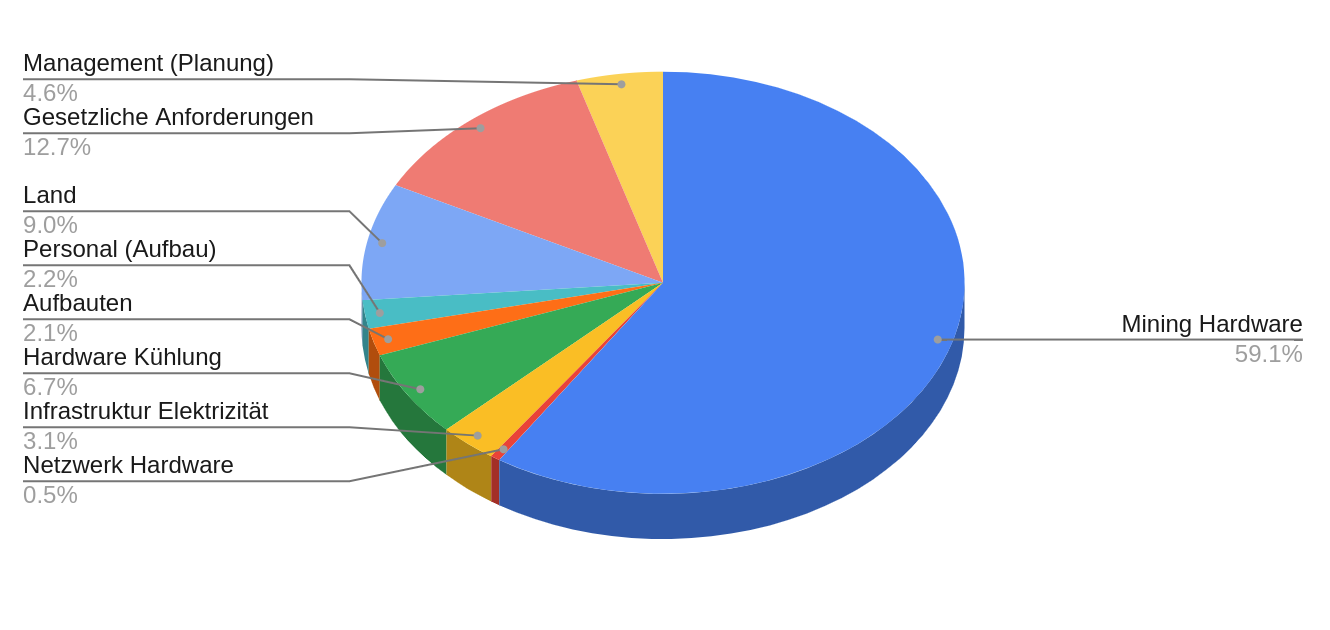
\includegraphics[width=0.7\textwidth]{capexdistribution10mw}
    \label{figure:capexdistribution10mw}
\end{figure}

In addition to the expenses that must be considered initially for a data center, the following costs (\ac{OpEx}),
which arise during operation, have to be considered:\footcite[Cf.][]{appendix:opex}
\begin{itemize}
    \item \textbf{Electricity: }This part describes the costs generated by the consumption of electricity.
    This parameter is a key component when considering \acp{KPI} of a cryptomining data center.
    (see Figure \ref{figure:valuechaindatacenter}).\footcite[Cf.][p. 327]{derks2018chaining} Since a mining data center
    is a bulk buyer from electricity, prices are subject to fluctuation, which is dictated by the provider\footcite[Cf.][]{appendix:opex}
    This item is one of the variable costs, since as the number of devices for mining and cooling increases.
    The annual cost for a 10MW data center at a base price of
    base price of $0.0357 \frac{USD}{kWh}$ circa 3,038,313 USD.\footcite[Cf.][]{appendix:opex}
    \item \textbf{Loan hardware charges: }This item carries equipment that is on loan and therefore must be paid for at regular
    periodic intervals. In the case of Genesis Group, this is the main distribution boards and transformers
    of a data center, which have a capacity greater than 1MW. Since this equipment is very expensive to purchase, it is borrowed from
    the energy suppliers. The annual cost of such a loan is about 170,280 USD for 10MW
    and are variable in nature.\footcite[Cf.][]{appendix:opex}
    \item \textbf{Spares: }In order to be able to repair defects of any hardware on site, the item of the
    spare parts is placed in the calculation for the \ac{OpEx}.\footcite[Cf.][p. 327]{derks2018chaining} For this part, there are
    no exemplary figures available.
    \item \textbf{Personnel: }To ensure that hardware can be repaired and data center operations
    can be maintained, personnel is required permanently on site. In the example, this item amounts to approx.
    31,282 USD per month, but can vary drastically from country to country.\footcite[Cf.][]{appendix:opex}
    This amount is listed under fixed costs because the initial size of the data center means that staffing plans are also
    is clear. No additional staff is hired even for small expansions.\footcite[Cf.][]{appendix:opex}
    \item \textbf{Management (Operations): }For the management of the data center and central project management, a
    flat rate of 6,289 USD per month is taken into place.\footcite[Cf.][]{appendix:opex} This describes
    the administrative costs from a central management point of view.
    \item \textbf{\ac{OBE}: }This area records the office costs, costs for the Internet, water and office electricity.
    These amount to approximately 3,593 USD per month for a 10MW data center and are fixed costs, as none of these items
    will change once the data center is up and running.\footcite[Cf.][]{appendix:opex}
\end{itemize}

\begin{figure}[H]
    \caption{OpEx distribution for a 10MW data center}
    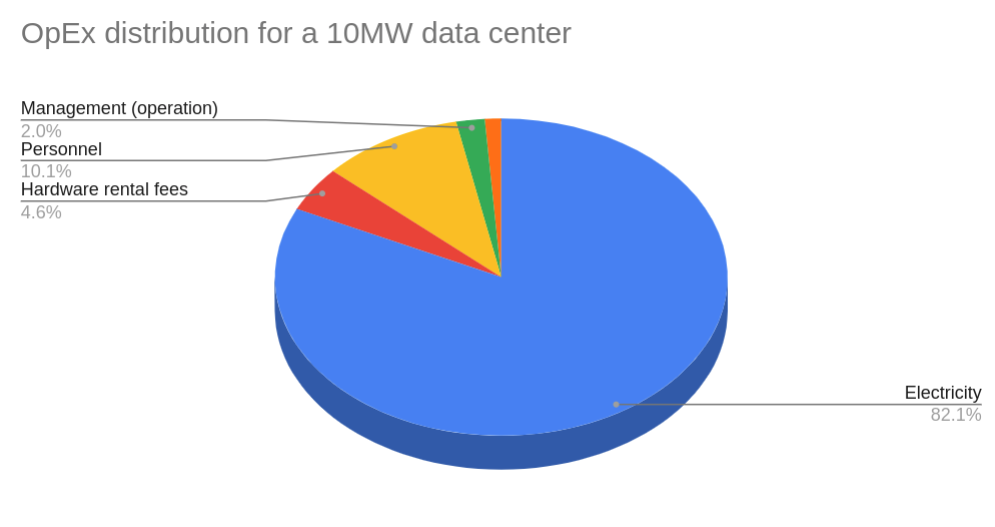
\includegraphics[width=0.7\textwidth]{opexdistribution10mw}
    \label{figure:opexdistribution10mw}
\end{figure}

In summary, for a mining capacity of 10MW, the \ac{OpEx} is approximately 317,897 USD.\footcite[Cf.][]{appendix:opex}
Now the mining has to generate revenues that amortize these expenses over time
so the company is able to make a profit. The distribution of the individual costs
is shown in Figure \ref{figure:opexdistribution10mw} relative on an annual basis.

Wie bereits in der Auszählung für \ac{CapEx} beschrieben, wird die finanzielle Effektivität eines Mining Gerätes durch
die Größe \RM betrachtet. Allerdings kann diese sehr stark fluktuieren, da dabei Faktoren, wie der Tauschkurs von Bitcoin
in USD (s. Ziffer "`Exchanges"' in Abb. \ref{figure:valuechaindatacenter}) und auch \DP, sich abhängig von den Mining
Parametern, wie Difficulty und Netzwerk Hashrate, entwickeln. Eine genaue Vorhersage ist daher nicht möglich, weshalb dort
mit verschiedenen Szenarien gerechnet wird.\footcite[Cf.][]{appendix:s19proassumptions} Aus diesen wird dann letztendlich ein
gewichteter Durchschnitt gebildet, welcher für die Kalkulation verwendet wird.\footcite[Cf.][]{appendix:s19proassumptions}

As already described in the count for \ac{CapEx}, the financial effectiveness of a mining device is
is considered by the size \RM. However, this can fluctuate greatly due to factors such as the exchange rate of Bitcoin
into USD (see figure "`Exchanges"' in Fig. \ref{figure:valuechaindatacenter}) and also \DP, vary depending on the mining
parameters, such as Difficulty and Network Hashrate. An exact prediction is therefore not possible, which is why
different scenarios are calculated.\footcite[Cf.][]{appendix:s19proassumptions} From these, a weighted average is finally formed.\footcite[Cf.][]{appendix:s19proassumptions}

\begin{figure}[H]
    \caption{Cost and value flows for a mining data center}
    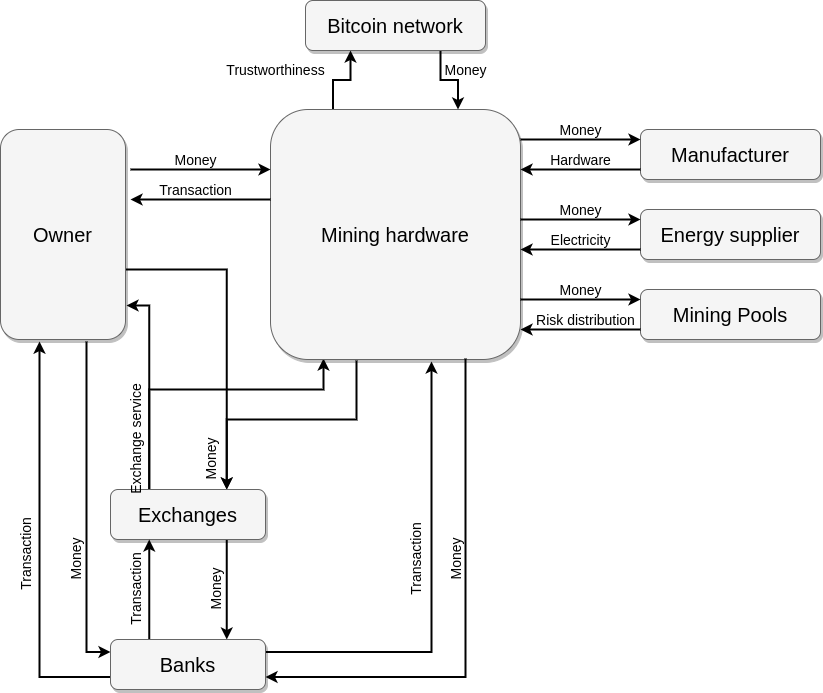
\includegraphics[width=0.7\textwidth]{valuechaindatacenter}
    \label{figure:valuechaindatacenter}
    \\
    \cite[Source: Based on][Fig. 3]{derks2018chaining}
\end{figure}

In the present example of the mining data center, the following scenarios were formed with probabilities of occurrence:

\begin{table}[H]
    \caption{Mining Effectiveness Scenarios}
    \label{tbl:miningrewardscenario}
    \begin{tabularx}{\textwidth}[ht]{X||X|X|X}
        Scenario & \RM & Probability of occurrence & Mining revenue  \\
        \hline\hline
        Worst-Case & $0,07\ USD / \frac{TH}{s} / day$ & $30\%$ & $8.224.610\frac{USD}{Year}$ \\
        \hline
        Most-Probable & $0,09\ USD / \frac{TH}{s} / day$ & $40\%$ & $10.574.499\frac{USD}{Year}$ \\
        \hline
        Optimal & $0,27\ USD / \frac{TH}{s} / day$ & $30\%$ & $31.723.497\frac{USD}{Year}$ \\
    \end{tabularx} \\
    \cite[Source: Based on][]{appendix:s19proassumptions}
\end{table}

As can be seen from table \ref{tbl:miningrewardscenario}, revenues fluctuate between 10 and over
30 million \ac{USD}, which is a considerable fuzziness. Therefore, optimization should be sought for these values.
Whether this is possible is evaluated in the following chapters. Furthermore, these calculations do not include any further
risks and will be ignored therefore. This also represents an opportunity for improvement,
since with an additional risk analysis the probabilities of occurrence can be better estimated.

Based on all financial data, cash flow and break-even point are calculable. The result of
such a calculation can be found in figure \ref{figure:datacentercashflow}. In the figure the respective values are
on an annual basis and show the development of \ac{CapEx} and \ac{OpEx} over the years.

\begin{figure}[H]
    \caption{Cash flow and break-even of a mining data center}
    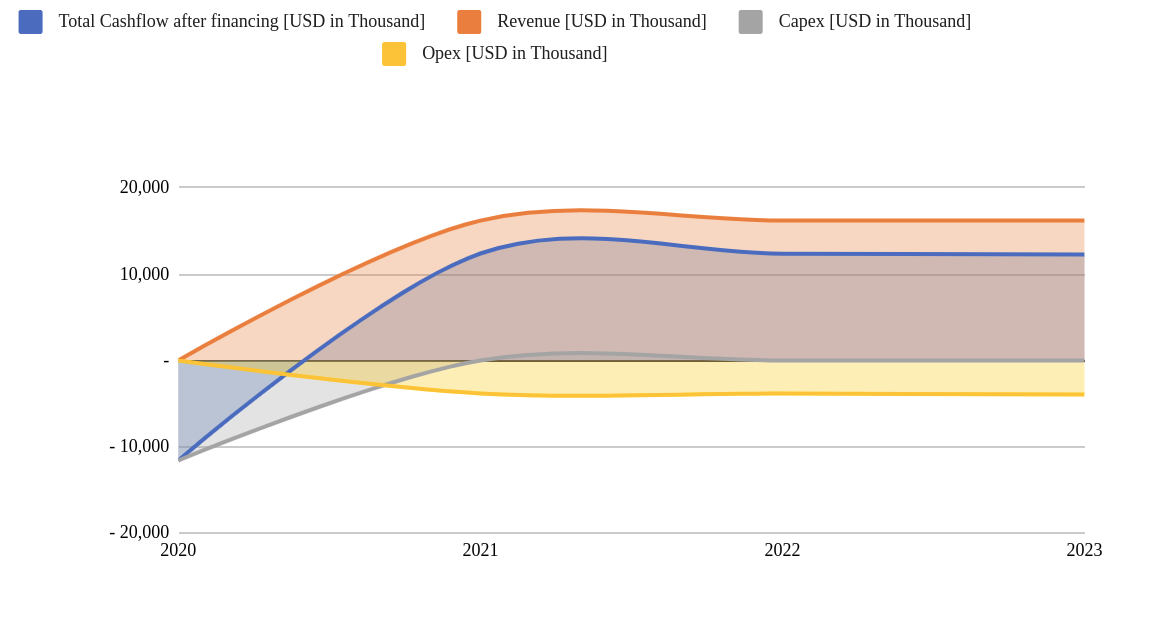
\includegraphics[width=0.7\textwidth]{datacentercashflow}
    \label{figure:datacentercashflow}
    \\
    \cite[Source: ][]{appendix:summaryofinvestment}
\end{figure}

Ultimately, there are other factors that influence the effectiveness of a data center and thus on the side of the
revenue side:
\begin{itemize}
    \item \textbf{Climate: }The climate affects the effectiveness of the miners and also significantly determines
    the dimensioning of the cooling. Accordingly, the goal in site selection is to find an optimal combination of
    electricity price, which largely determines the \ac{OpEx}, and the \ac{CapEx} for cooling, which accounts for a
    large share. However, the exact climate is not included in considerations.
    \item \textbf{Supply security: }This factor describes the security of the necessary external infrastructure,
    such as Internet and electricity. Since every failure inevitably leads to an effective complete breakdown of the data center,
    this must be included in the consideration.
\end{itemize}
\newpage
\section{Anwendbarkeit von Business Intelligence auf Kryptomining Rechenzentren} \label{toc:ansatzmoeglichkeitenfuerbusinessintelligence}

In diesem Kapitel wird die Anwendbarkeit der Prinzipien von \ac{BI} Prozessen auf Kryptomining Rechenzentren geprüft, um eine
finanzielle Optimierung der Rechenzentren zu erreichen. Ziel dieses Teils ist die Prüfung der in Kapitel
\ref{toc:hypothesenundabgrenzungderarbeit} formulierten Teilhypothesen. Damit ist es möglich, letztendlich eine Aussage über
die Haupthypothese treffen zu können. Um in der Lage zu sein, Aussagen am Schluss formulieren zu können, wird als Methodik die
argumentative-deduktive Analyse verwendet. Diese Methodik ist qualitativer Natur und gehört zu den konstruktionswissenschaftlichen
Methoden.\footcite[Vgl.][S. 283f]{wilde2007forschungsmethoden} Es werden aus vorhergehenden Schlussfolgerungen deduktiv weitere
Aussagen abgeleitet, die am Ende zur Beantwortung der Haupthypothese dieser Arbeit
führen.\footcite[Vgl.][S. 7]{wilde2006methodenspektrum} Als Basis für die Deduktion werden die erarbeiteten Grundlagen aus
Kapitel \ref{toc:grundlagenbusinessintelligence} und Kapitel \ref{toc:grundlagenkryptomining} verwendet. Im ersten Teil
dieses Kapitels werden  vertieft die \acp{KPI} aus Kapitel \ref{toc:grundlagenkryptomining} verwendet und deren Ursprung
betrachtet. Diese grundlegenden Daten werden nach verschiedenen Gesichtspunkten, wie Verfügbarkeit, Echtzeitcharakter,
Qualität, Datenänderungsrate und Quantität klassifiziert und damit deren Eignung für \ac{BI} Prozesse betrachtet. Die Daten
werden folgend nach internen und externen Quellen unterteilt. Schlussendlich ist der Leser in der Lage zu verstehen, welche
Daten zur Verfügung stehen und wie diese sich für \ac{BI} eignen. In Kapitel \ref{toc:pruefungderteilhypothesen} wird
die eigentliche Prüfung der vier Teilhypothesen durchgeführt. Dabei werden im ersten Schritt die relevanten \acp{KPI}
identifiziert, die für die eigentliche erfolgreiche Prüfung der Teilhypothesen benötigt werden. Im zweiten Schritt werden
die Analyseverfahren dahingehend betrachtet, ob aus den grundlegenden Daten jeder der relevanten \acp{KPI} errechnet werden kann.
Schlussendlich ist es damit möglich, die Teilhypothesen zu verifizieren und eine Aussage in Kapitel 
\ref{toc:zusammenfassendebetrachtung} auf der Ebene der Haupthypothese treffen zu können.

\subsection{Klassifizierung der verfügbaren Daten} \label{toc:klassifizierungderdaten}

Wie in der Einleitung des Hauptkapitels beschrieben, werden in diesem Teil die verfügbaren Datenquellen identifiziert und
kategorisiert. Mit Hilfe dieser Einteilung wird die Eignung der Daten für \ac{BI} bestimmt. Die zusammenfassenden Ergebnisse
dieses Kapitels finden sich in Tabelle \ref{tbl:klassifizierunginternedaten} und Tabelle \ref{tbl:klassifizierungexternedaten}.

\begin{figure}[H]
    \caption{Klassifizierung von Datenquellen}
    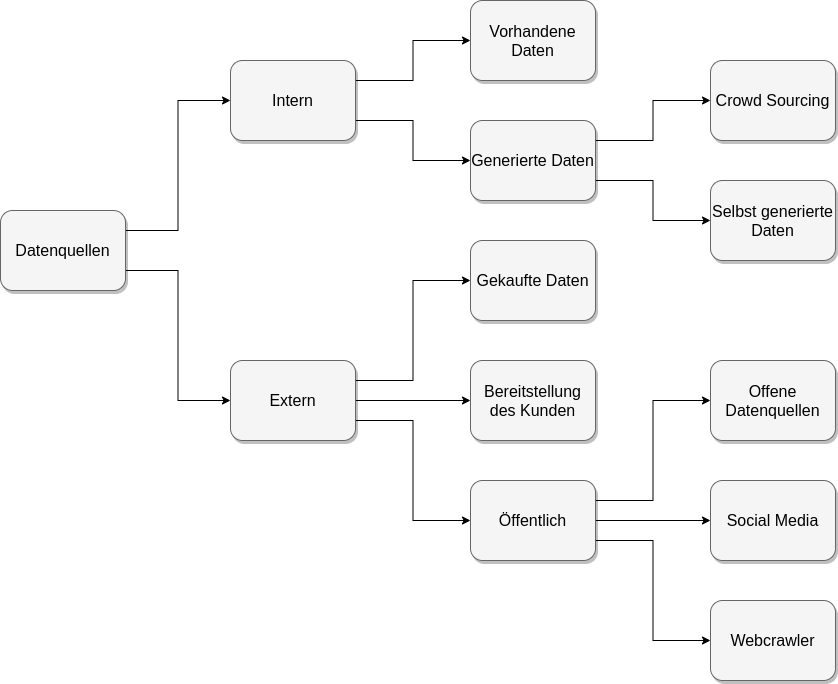
\includegraphics[width=0.7\textwidth]{datasources}
    \label{figure:datasources}
    \\
    \cite[Quelle: In Anlehnung an][Abb. 1]{hartmann2016capturing}
\end{figure}

Auf Basis von Abbildung \ref{figure:datasources} ist in der ersten Ebene eine Einteilung der Daten in interne und externe
Datenquellen möglich. Diese Unterteilung beschreibt die Herkunft der Daten.\footcite[Vgl.][Abb. 1]{hartmann2016capturing}
Interne Datenquellen stellen Daten zur Verfügung, die ausschließlich innerhalb einer Organisation zugänglich sind. Zu diesen
Datenquellen zählen folgend Daten der Mining Hardware, von \ac{ERP} Systemen und der Personalplanung. Bei den externen
Datenquellen gibt es eine dreiteilige Unterscheidung in gekaufte Daten, Daten, die durch einen Kunden bereitgestellt werden,
und öffentlich verfügbare Daten. Bei dieser Unterscheidung werden in Kapitel \ref{toc:externedatenquellen} primär die
öffentlichen Datenquellen betrachtet, da im Betrieb von Kryptomining Rechenzentren der Kundenfaktor erstmal ignoriert werden
kann. Zu diesen Datenquellen zählen öffentliche Blockexplorer, Mining Pools, Tauschbörsen, Wetter- und Klimadaten sowie
Daten aus Social Media Plattformen. Die Daten werden nach den folgenden Eigenschaften hin analysiert:
\begin{itemize}
    \item \textbf{Datenstruktur: }Daten können in strukturierte und unstrukturierte Daten unterteilt werden. Beispiele für
    strukturierte Daten sind Finanzdaten oder Sensordaten.\footcite[Vgl.][S. 27]{kimble2015big} Unstrukturierte Daten
    können Bilder, Texte oder Daten aus Social Media Plattformen sein.\footcite[Vgl.][S. 27]{kimble2015big}Diese Unterteilung
    hat Einfluss auf den \ac{ETL} Prozess, da Data Warehouses ausschließlich strukturierte Daten abspeichern
    können.\footcite[Vgl.][S.21]{niu2009cognition} Im Falle der Verwendung von unstrukturierten Daten müssen diese so angepasst
    werden, dass sie strukturiert werden.
    \item \textbf{Verfügbarkeit: }Mit diesem Parameter wird die Dauer von der Erhebung eines Datenpunktes bis hin zur
    Verfügbarkeit für Nutzer der Software gemessen. Gerade auf die Analyseprozesse kann dieser Parameter Auswirkungen
    haben, da dieser entscheidet, ob ein System benötigt wird, dass Echtzeitdaten verarbeiten muss oder beispielsweise nur
    Stapelverarbeitung betreibt. Die Ergebnisse aus dieser Kategorie werden in der Einschätzung der in Frage kommenden
    Analyseprozesse in Kapitel \ref{toc:analyseverfahrenbi} verwendet.
    \item \textbf{Konsistenz: }Diese Metrik sagt aus, ob die Daten, die durch die Quellsysteme zur Verfügung gestellt werden,
    frei von Widersprüchen sind. Falls Daten nicht widerspruchsfrei sind, kann dies zu Fehlern in den Analyseprozessen führen,
    die daher genau beobachtet werden müssen.\footcite[Vgl.][S. 561]{huh1990data} Da das Auswirkungen auf die Gestaltung
    der Analyseprozesse hat, muss diese Tatsache mit in Betracht gezogen werden.
\end{itemize}

\subsubsection{Interne Datenquellen} \label{toc:internedatenquellen}

In diesem Teil werden die internen Datenquellen und deren Daten klassifiziert, die für die Konzeption eines \ac{BI} Prozesses
in Betracht gezogen werden können.

\begin{itemize}
    \item \textbf{Mining Hardware / Überwachungssoftware: }
    Die technischen Parameter während des Betriebes werden durch die Mining Hardware generiert. Diese Parameter lassen
    Rückschlüsse auf die Effektivität der Hardware während des Mining Prozesses zu. Dazu zählen Daten, wie Hashrate, Temperatur,
    Hardwaredefekte und Stromverbrauch.\footcite[Vgl.][S. 12]{antminer2021manual} Diese Metriken sind über \acp{API} oder
    durch die \ac{SSH} Schnittstelle abfragbar.\footcite[Vgl.][]{awesomeminer2021api} Da die Konfiguration und Überwachung
    vieler einzelner Geräte einen zu hohen Aufwand und Zeitverbrauch für das Personal darstellt, wird Software eingesetzt,
    die in der Lage ist, eine große Anzahl von Mining Geräten zu überwachen und zu konfigurieren. Um dies zu erreichen, wird
    die \ac{API} oder \ac{SSH} Schnittstelle der Mining Hardware verwendet. Durch den Einsatz der Software können auch die
    Ausfallszeiten der Mining Hardware und der Stromverbrauch der Kühlung eines Rechenzentrums gemessen werden. Zusätzlich
    wird diese Software durch das Wartungspersonal verwendet, um defekte Geräte ausfindig zu machen und diese zu reparieren.
    Die Informationen zur Reparatur werden durch das Personal in das System eingetragen.
    \begin{itemize}
        \item Datenstruktur: Da es sich bei den Daten, welche die Mining Hardware generieren und die in der Überwachungssoftware
        gesammelt werden, letztendlich ausschließlich um Sensordaten handelt, sind die Daten aus dieser Quelle
        strukturiert.\footcite[Vgl.][S. 27]{kimble2015big}
        \item Verfügbarkeit: Die Verfügbarkeit der Daten in der Überwachungssoftware liegt bei circa fünf bis zehn Minuten,
        da diese Daten über regelmäßige Stapelverarbeitungsprozesse abgefragt werden.
        \item Konsistenz: Die Konsistenz ist gegeben. Alle diese Daten werden in relationalen Zeitreihen gespeichert. 
    \end{itemize}
    \item \textbf{ERP System: }Finanzielle \acp{KPI} werden meist in \ac{ERP} Systemen
    gespeichert.\footcite[Vgl.][Tabelle 3]{spathis2003usefulness} Diese Systeme werden dafür benutzt, die finanziellen \acp{KPI}
    eines Rechenzentrums zu erhalten. Diese Daten sind beispielsweise Anschaffungskosten, Kosten des Managements,
    Elektrizitätskosten und Personalkosten. Eine ausführliche Auflistung findet sich in
    Kapitel \ref{toc:kennzahlenundeinflussfaktoren}. In den folgenden Betrachtungen werden diese Daten in die Kategorien
    \ac{CapEx} und \ac{OpEx} aufgeteilt, da dies für die Prüfung der Hypothesen ausreichend ist. Durch die Schnittstellen
    der ERP Systeme sind diese Daten einheitlich abfragbar.
    \begin{itemize}
        \item Datenstruktur: Da es sich bei diesen Daten vorrangig um Finanzdaten handelt und diese durch die Schnittstelle
        des ERP Systems abgefragt werden, handelt es sich um strukturierte Daten.\footcite[Vgl.][S. 27]{kimble2015big}
        \item Verfügbarkeit: Sobald diese Daten in einem \ac{ERP} System eingetragen sind, sind diese auch direkt abfragbar.
        Daher bietet ein \ac{ERP} System Echtzeitdaten an.
        \item Konsistenz: Ausgehend von der Annahme, dass die eingehenden Daten korrekt sind, sind die Informationen aus
        einem \ac{ERP} System widerspruchsfrei und damit konsistent.
    \end{itemize}
    \item \textbf{Personalplanung: }Letztendlich sind die Planungssysteme für das Personal intern verfügbar. Diese
    beinhalten die Zahl der Angestellten, deren Gehälter und deren Arbeitszeiten. Zusätzlich zu den Arbeitszeiten sind die
    Schichtpläne der Rechenzentren in diesen Systemen verfügbar, worüber Schlussfolgerungen über die Personalbeschaffenheit
    vor Ort gemacht werden können. Diese Daten sind über standardisierte Schnittstellen abfragbar.
    \begin{itemize}
        \item Datenstruktur: Die Daten, die das Personalsystem zur Verfügung stellt, sind strukturiert und relational.
        \item Verfügbarkeit: Die Verfügbarkeit solcher Daten ist direkt und ohne Zeitverzögerung abfragbar, sobald diese in
        das System eingetragen sind.
        \item Konsistenz: Unter der Voraussetzung, dass alle eingegebenen Daten korrekt sind, sind alle Daten eines
        Personalmanagementsystems widerspruchsfrei.
    \end{itemize}
\end{itemize}

In der folgenden Tabelle sind die Klassifizierungen der einzelnen Datentypen gelistet, die sich aus den oben genannten Datenquellen
ergeben.

\begin{table}[H]
    \caption{Klassifizierung der internen Datenquellen}
    \label{tbl:klassifizierunginternedaten}
    \begin{tabularx}{\textwidth}[ht]{X||c|c|c}
        Datenquelle & Datenstruktur & Verfügbarkeit & Konsistenz  \\
        \hline\hline
        Mining Hardware / Überwachungssoftware & Strukturiert & 5-10 Minuten & Konsistent \\
        \hline
        ERP System & Strukturiert & \specialcell{Echtzeit innerhalb\\der Software} & Konsistent \\
        \hline
        Personalplanung & Strukturiert & \specialcell{Echtzeit innerhalb\\der Software} & Konsistent \\
    \end{tabularx}
\end{table}

\subsubsection{Externe Datenquellen} \label{toc:externedatenquellen}

Analog zur Klassifizierung der internen Daten in Kapitel \ref{toc:internedatenquellen}, werden im Folgenden die externen
Datenquellen klassifiziert. Die folgenden relevanten externen Datenquellen sind identifizierbar:

\begin{itemize}
    \item \textbf{Öffentliche Blockexplorer: }Blockexplorer sind Webseiten, die die Daten der Blockchain über Schnittstellen
    abrufbar machen. Beispiele für Daten, die direkt auf der Blockchain liegen, sind die Difficulty oder auch die Höhe der
    Transaktionsgebühren der noch nicht bestätigten
    Transaktionen.\footcite[Vgl.][]{bitcoin2021getdifficulty}\footcite[Vgl.][]{bitcoin2021getrawmempool} Zusätzlich werden
    Metriken angeboten, die auf Basis der Daten auf der Blockchain berechnet oder abgeschätzt werden können. Dazu gehören
    Daten wie beispielsweise die Schätzung der Netzwerkhashrate des Bitcoin
    Netzwerks.\footcite[Vgl.][]{blockchain2021total}\footcite[Vgl.][]{blockchain2021api} Zusätzlich können über solche
    Blockexplorer auch jegliche blockchainbezogenen Daten in ihrer vollen Historie bezogen werden. Eine andere Möglichkeit,
    die Daten der Blockchain zu erhalten, wäre der Betrieb einer eigenen Bitcoin Node. Da der Betrieb und die Wartung davon
    viel Fachwissen verlangt, ist die Abfrage der Daten durch einen öffentlichen Blockexplorer zu bevorzugen.
    \begin{itemize}
        \item Datenstruktur: Die Beschaffenheit der Daten, die von einem Blockexplorer geliefert werden, sind strukturiert.
        Dies liegt vor allem an der strikten Strukturiertheit der Blockchain.
        \item Verfügbarkeit: Die Verfügbarkeit unterscheidet sich je nach abgefragten Parametern. Daten, die direkt auf
        der Blockchain gespeichert sind, sind in Echtzeit abfragbar. Beispiele dafür ist die Difficulty oder Informationen
        über Transaktionen.
        
        Alle weiteren Daten, die auf Basis der Blockchaindaten errechnet werden, aber nicht direkt von dieser stammen, werden
        meist nur einmal am Tag veröffentlicht. Ein Beispiel ist die hochgerechnete Gesamthashrate des Bitcoin Netzwerks.
        \item Konsistenz: Da die Widerspruchsfreiheit der Daten einer der Gründe für die Einführung von Blockchains waren,
        können folglich die Daten eines Blockexplorers auch als widerspruchsfrei und damit konsistent angesehen werden. 
    \end{itemize}
    \item \textbf{Mining Pools: }Wie in Kapitel \ref{toc:miningundkonsensalgorithmen} bereits gezeigt, gibt es die
    Möglichkeit, durch Mining Pools am Mining teilzunehmen. Ein Mining Pool bietet die Möglichkeit der Risikoreduzierung
    während des Mining Prozesses. Dafür verlangt dieser Nutzungsgebühren, die unterschiedlich bemessen sein
    können.\footcite[Vgl.][S. 59ff]{bhaskar2015bitcoin} Diese Gebühren können direkt von einem Mining Pool abgefragt werden
    und damit in die finanzielle Gesamteinschätzung Einzug halten. Da der Besitzer der Mining Hardware anteilig
    zu der zur Verfügung gestellten Hashrate am Ertrag des Pools beteiligt wird, ist bei einem Mining Pool die ankommende
    Hashrate nachvollziehbar. Diese kann mit der Hashrate der Mining Hardware verglichen werden, um Aussagen über die
    Netzwerkverbindungen treffen zu können. Alle diese Daten sind standardisiert über eine \ac{API} erhältlich.
    \begin{itemize}
        \item Datenstruktur: Die Daten über die Hashrates sind vergleichbar zu Sensordaten. Aus diesem Grund liefert ein
        Mining Pool strukturierte Daten aus.\footcite[Vgl.][S. 27]{kimble2015big}
        \item Verfügbarkeit: Die Daten sind mit einer Verzögerung von 15-30 Minuten abfragbar.
        \item Konsistenz: Die Daten sind konsistent, da diese auf der Basis von Zeitreihen erhoben werden. Es können
        Unterschiede zur Hashrate der Mining Hardware gemessen werden. Diese sind allerdings keine Inkonsistenz, sondern
        geben Rückschlüsse auf die Verbindungsqualität zwischen Rechenzentrum und Mining Pool.
    \end{itemize}
    \item \textbf{Tauschbörsen: }Die Tauschbörsen werden verwendet, um die durch den Mining Prozess verdienten Bitcoins in
    Fiat Währungen umtauschen zu können. Dabei sind zwei Hauptfaktoren zu beachten. Das ist zum einen der momentane Tauschkurs
    zwischen \ac{BTC} und \ac{USD}. Zum anderen müssen die Handelsgebühren einer Tauschbörse noch zusätzlich in Betracht
    gezogen werden. Alle diese Werte unterscheiden sich von Börse zu Börse. Tauschbörsen haben umfangreiche und
    performante \acp{API}, um mit diesen sehr schnell handeln zu können.
    \begin{itemize}
        \item Datenstruktur: Tauschbörsen bieten strukturierte Daten an. Nur diese Form der Daten lässt eine sehr schnelle
        Bearbeitung und Analyse zu.\footcite[Vgl.][S. 27]{kimble2015big}
        \item Verfügbarkeit: Die Schnittstellen der Börse stellen Daten in Echtzeit bereit.
        \item Konsistenz: Die Daten der Tauschbörsen müssen konsistent sein, da sonst Probleme im Handel auftreten können.
    \end{itemize}
    \item \textbf{Wetter- und Klimadaten: }Betreiber von Kryptomining Rechenzentren sind durch die dynamische Anpassung der
    Kühlungsanlagen an die Außentemperatur in der Lage, Energiekosten einzusparen. Um dieses Einsparungspotential nutzen zu
    können, werden Schnittstellen benötigt, an denen aktuelle und historische Wetterdaten abfragbar sind. Ein Beispiel für
    eine umfassende Schnittstelle ist World Weather Online.\footcite[Vgl.][]{wwo2021api} Diese Schnittstelle verlangt ein Entgelt
    für die Nutzung, da die Bereitstellung von weltweiten Wetterdaten komplex ist.\footcite[Vgl.][]{wwo2021pricing} Gerade bei
    einem Neubau eines Rechenzentrums macht die Einbeziehung von Klimadaten Sinn, um den Stromverbrauch und die Dimensionierung
    der Kühlungsanlagen abschätzen zu können.
    \begin{itemize}
        \item Datenstruktur: Wetter- und Klimadaten werden strukturiert zur Verfügung gestellt, um eine gute Analyse ermöglichen
        zu können.
        \item Verfügbarkeit: Die Daten werden laut World Weather Online in Echtzeit zur Verfügung
        gestellt.\footcite[Vgl.][]{wwo2021api}
        \item Konsistenz: Die Konsistenz der Daten ist wichtig und innerhalb einer Plattform auch gegeben. Bei der Abfrage
        mehrerer Quellen für Wetterdaten kann es zu Inkonsistenzen kommen.
    \end{itemize}
    \item \textbf{Social Media: }Anfang des Jahres 2021 war beobachtbar, dass durch Social Media Plattformen der Bitcoin
    Wechselkurs stark beeinflusst wurde
    (Vgl. Abb. \ref{figure:btctweets}).\footcite[Vgl.][]{forbes2021musk}\footcite[Vgl.][S. 1f]{ante2021elon} Daher darf in
    einer Einschätzung der Wechselkurse der Einfluss von Social Media inzwischen nicht mehr ignoriert werden. In Social Media
    ist es durch die Analyse von beispielsweise Hashtags möglich, ein Stimmungsbild zu ermitteln. Auch können Äußerungen von
    reichweitenstarken Personen oder Gruppen, die kursbeeinflussend sind, schnell analysiert werden.
    \begin{itemize}
        \item Datenstruktur: Die Daten von Social Media Plattformen sind unstrukturiert.\footcite[Vgl.][S. 27]{kimble2015big}
        \item Verfügbarkeit: Die Verfügbarkeit von Daten über Web Scraping oder \acp{API} ist in Echtzeit gegeben.
        \item Konsistenz: Da an Social Media Plattformen grundsätzlich jeder Mensch teilnehmen kann, sind die Daten, die
        analysiert werden können, inkonsistent.
    \end{itemize}
\end{itemize}

\begin{figure}[H]
    \caption{Bitcoin Wechselkurs im Vergleich mit den Anzahl der Tweets mit Hashtag \#bitcoin pro Tag}
    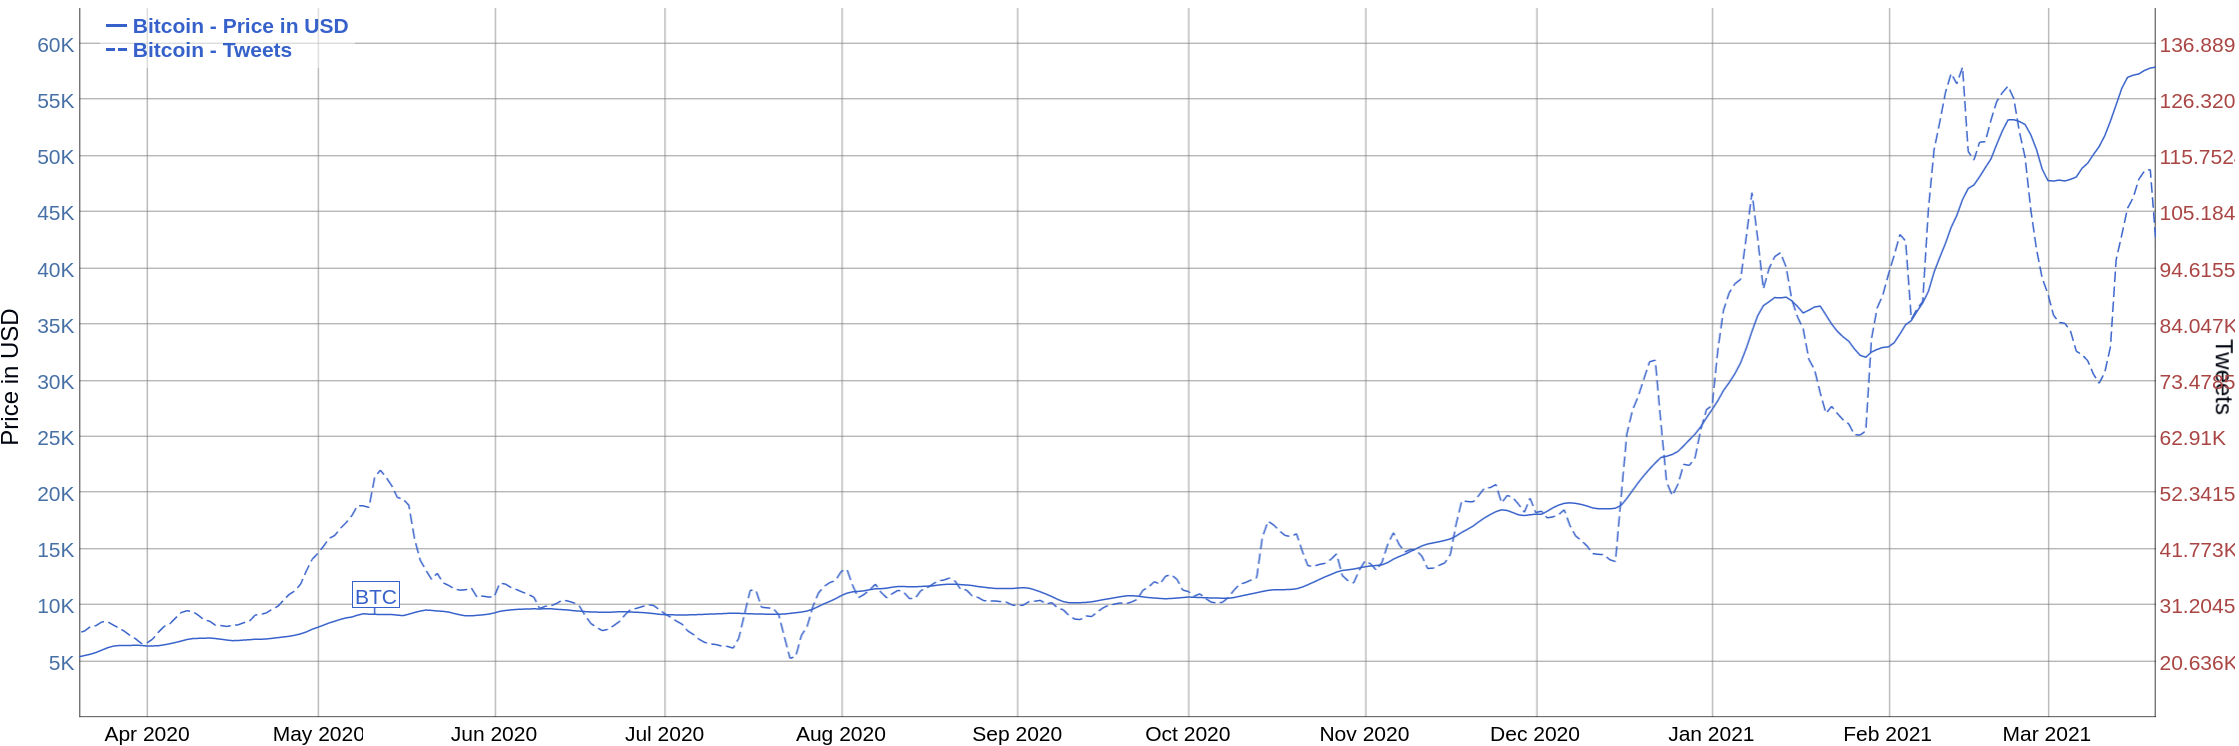
\includegraphics[width=\textwidth]{tweetsbitcoin}
    \label{figure:btctweets}
    \\
    \cite[Quelle: Vgl.][]{bitinfocharts2021bitcointweets}
\end{figure}

Zusammenfassend sind die erarbeiteten Klassifizierungen in Tabelle \ref{tbl:klassifizierungexternedaten} aufgelistet.

\begin{table}[H]
    \caption{Klassifizierung der externen Datenquellen}
    \label{tbl:klassifizierungexternedaten}
    \begin{tabularx}{\textwidth}[ht]{X||c|c|c}
        Datenquelle & Datenstruktur & Verfügbarkeit & Konsistenz  \\
        \hline\hline
        Öffentliche Blockexplorer (Daten der Blockchain) & Strukturiert & Echtzeit & Konsistent \\
        \hline
        Öffentliche Blockexplorer (Metriken basierend auf Blockchaindaten) & Strukturiert & 24 Stunden & Konsistent \\
        \hline
        Mining Pools & Strukturiert  & 15-30 Minuten & Konsistent \\
        \hline
        Tauschbörsen & Strukturiert & Echtzeit & \specialcell{Konsistent innerhalb\\jeder Tauschbörse} \\
        \hline
        Wetter- und Klimadaten & Strukturiert & Echtzeit & \specialcell{Konsistent innerhalb\\jedes Wetterdienstes} \\
        \hline
        Social Media & Unstrukturiert & Echtzeit & Inkonsistent \\
    \end{tabularx}
\end{table}

\subsection{Prüfung der Teilhypothesen} \label{toc:pruefungderteilhypothesen}

Basierend auf der Klassifizierung der möglichen Datenquellen und deren verfügbaren Informationen wird in diesem Teil die Prüfung
der Teilhypothesen vorgenommen. Dazu wird für jede einzelne Teilhypothese definiert, welche \acp{KPI} relevant sind, um diese
zu evaluieren und final zu verifizieren. Dafür werden die \acp{KPI} aus den Kapiteln \ref{toc:technologie} und
\ref{toc:miningrechenzentren} verwendet. Zusätzlich werden die Ergebnisse über die verfügbaren Datenquellen aus Kapitel
\ref{toc:klassifizierungderdaten} mit einbezogen, um Datenflüsse für eine \ac{BI} Implementierung zu identifizieren. Diese
werden für die Beantwortung der Hypothese verwendet. Abbildung \ref{figure:ht01dataflow} bis \ref{figure:ht04dataflow} machen
es möglich zu prüfen, welche Daten benötigt werden, ob diese für \ac{BI} verwendbar sind und ob diese zur Verfügung stehen.
In Kapitel \ref{toc:analyseverfahrenbi} wird besprochen, welche Analyseverfahren für die Daten benötigt werden, um letztendlich
die Teilhypothesen evaluieren und prüfen zu können. Dabei wird auch auf die verschiedenen Arten von \ac{BI} - deskriptive
(descriptive), vorhersagende (predictive) und präskriptive (prescriptive) Business Intelligence - und deren mögliche
Limitationen im Bereich Kryptomining eingegangen.\footcite[Vgl.][S. 96]{bihani2014comparative}

\subsubsection{Identifikation der Key Performance Indikatoren der Hypothesen} \label{toc:identifikationkpi}

Wie in der Einleitung zu diesem Kapitel bereits geschrieben, werden in diesem Teil die Datenquellen und die logischen Datenflüsse
identifiziert. Dazu werden alle vier Teilhypothesen getrennt betrachtet und jeweils ein zugeschnittener Abhängigkeitsbaum der
Informationen und \acp{KPI} definiert. Diese finden sich zusammengefasst in den jeweiligen Abbildungen, die zu den Teilhypothesen
gehören. Generell wird zwischen finanziellen, technischen und personellen \acp{KPI} unterschieden. Dahinter werden die
dementsprechenden Datenquellen aus Kapitel \ref{toc:klassifizierungderdaten} genannt, die von Relevanz sind. In der letzten Ebene
werden die einzelnen Datentypen, die benötigt werden, benannt. Im Folgenden wird diese Analyse für alle vier Teilhypothesen
durchgeführt:

\begin{itemize}
    \item \textbf{\ac{HT0.1}: }Diese Teilhypothese prüft einen möglichen Einfluss von \ac{BI} auf Entscheidungsprozesses des
    Managements in Bezug auf den Neu- und Ausbau von Kryptomining Rechenzentren. Eine solche Entscheidungsunterstützung benötigt
    eine Vielzahl an Daten, da ein Neu- oder Ausbau eine komplexe strategische Entscheidung darstellt. Aus diesem Grund werden alle
    drei Formen von \acp{KPI} - personelle, technische und finanzielle - benötigt.
    
    Diese strategische Entscheidung basiert auf Faktoren hinsichtlich des Ortes, der Auswahl der Hardware und der
    Tauschgeschäfte von Bitcoin in Fiat Währungen, um die Rechenzentren zu finanzieren. Die Auswahl des Ortes beeinflusst
    jegliche Formen der bereits beschriebenen \acp{KPI} und beruht damit auf Daten, wie Personalgehälter, \ac{CapEx}, \ac{OpEx}
    und Energieverbrauch der Mining Hardware. Die Auswahl der Hardware wiederum wird durch Faktoren, wie Hashrate, Ausfallszeiten
    (Stabilität der Hardware) und dem Energieverbrauch, bestimmt. Die Tauschgeschäfte werden durch die Daten, die Tauschbörsen
    anbieten, maßgeblich bestimmt.
    
    Nach Tabelle \ref{tbl:klassifizierunginternedaten} und \ref{tbl:klassifizierungexternedaten} sind alle diese Daten
    strukturiert und konsistent. Daher eignen sich diese Datenquellen ohne weiteres für die Verwendung in \ac{BI} Prozessen.
    Der \ac{ETL} Vorgang für die einzelnen Datenquellen lässt sich durch die genannten Grundeigenschaften der Daten problemlos
    aufbauen, damit die Daten durch ein Data Warehouse für die weiteren Teilprozesse verfügbar gemacht werden. Die Verfügbarkeit
    der verwendeten Daten unterscheidet sich je nach Datentyp. Bei Tauschbörsen sind die Daten direkt in Echtzeit abfragbar.
    Im Gegensatz dazu gibt es bei den technischen \acp{KPI} eine Verzögerung von circa fünf bis zehn Minuten.  Systeme wie
    \ac{ERP} und Personalerfassung liefern Daten in Echtzeit, sobald diese dem System vorliegen. Da strategische Entscheidungen,
    wie der Neu- oder Ausbau von Mining Rechenzentren, allerdings langwierige Entscheidung sind, limitiert die Verfügbarkeit
    die Hypothese nicht.

    Anhand der nun verfügbaren Daten wird im folgenden Kapitel evaluiert, ob es möglich ist, diese Daten in einer Art und Weise zu
    analysieren, sodass am Ende daraus zusätzliches Wissen generiert werden kann und damit diese Daten zur Entscheidungsunterstützung
    verwendet werden können.

    \begin{figure}[H]
        \caption{Relevante KPIs, Datenquellen und Datentypen für Teilhypothese 1}
        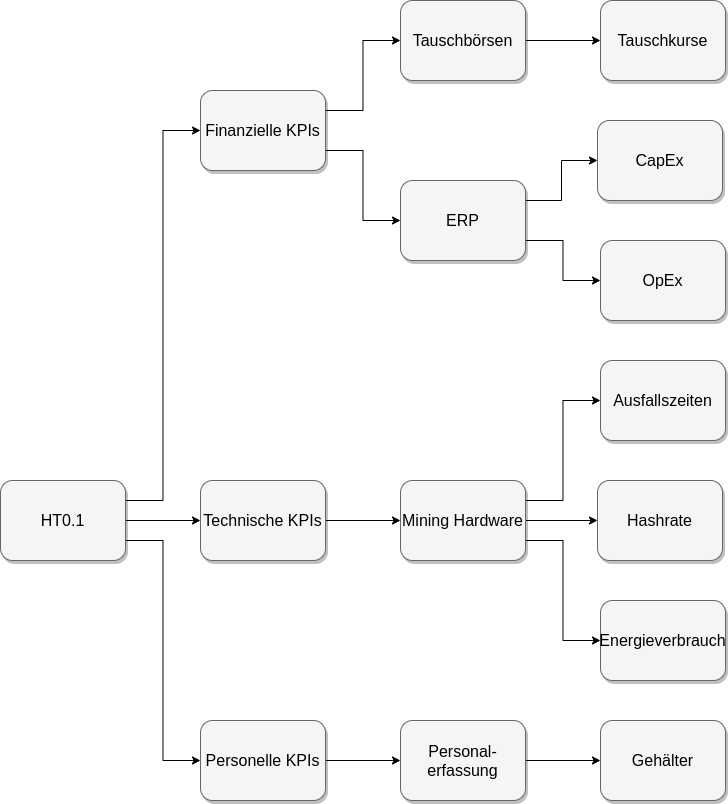
\includegraphics[width=0.55\textwidth]{ht01dataflow}
        \label{figure:ht01dataflow}
    \end{figure}

    \item \textbf{\ac{HT0.2}: }Diese Teilhypothese beschäftigt sich mit dem Einfluss von \ac{BI} auf die Effektivität der
    Mining Hardware. Da diese Hypothese ausschließlich technischer Natur ist, werden dafür nur technische \acp{KPI}, wie
    Stromverbrauch, Hashrate, Ausfallszeiten und Hardwaredefekte, benötigt. Diese Daten stammen ausschließlich aus dem
    Überwachungssystem der Mining Hardware. Nach Tabelle \ref{tbl:klassifizierunginternedaten} sind diese Daten sowohl
    konsistent als auch strukturiert, wodurch sich diese Daten für ein \ac{BI} Konzept eignen. Die \ac{ETL} Pipelines sind
    für diese Art von Daten einfach zu errichten. Die verzögerte Verfügbarkeit der Daten (fünf bis zehn Minuten) stellt keine
    Probleme für die Hypothese dar, da diese nicht zwingend auf Echtzeitdaten angewiesen ist. Gerade bei der Messung von
    Effektivitäten im Mining Prozess braucht man längere Zeitfenster von mehreren Tagen, um belastbare Aussagen zu erhalten.
    Anhand der Datenquellen können Faktoren berechnet werden, die Einfluss auf die Effektivität des Mining Prozesses haben.
    Dazu gehören die Hashrate der eigenen Mining Hardware, deren Energieeffizienz ("`Reference power effiency"',
    $\frac{J}{TH}$) und die Messung der Uptime und der Gerätedefekte, die beispielsweise durch bessere Firmwares optimiert
    werden können.

    \begin{figure}[H]
        \caption{Relevante KPIs, Datenquellen und Datentypen für Teilhypothese 2}
        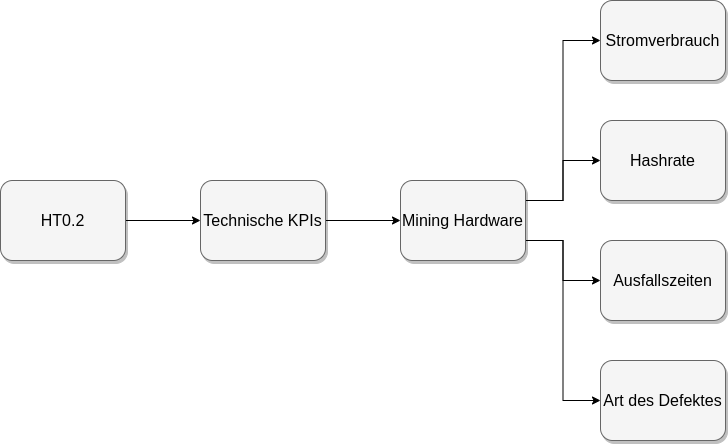
\includegraphics[width=0.55\textwidth]{ht02dataflow}
        \label{figure:ht02dataflow}
    \end{figure}

    \item \textbf{\ac{HT0.3}: }Die dritte Teilhypothese beschreibt die Verbesserung des Cashflows eines Kryptomining
    Rechenzentrums durch die Anwendung von \ac{BI}. Um die Hypothese zu prüfen, werden technische und finanzielle \acp{KPI}
    benötigt. Unter den technischen \acp{KPI} finden sich Parameter, wie Hashrate und Informationen aus öffentlichen
    Blockexplorern, wie beispielsweise die Difficulty und die Hochrechnung der Netzwerkhashrate. Durch diese Informationen ist
    der theoretische Mining Ertrag durch die Hardware prognostizierbar. Die finanziellen \acp{KPI} teilen sich in Tauschbörsen,
    \ac{ERP} Systeme und Mining Pools auf. Die Tauschbörsen liefern Daten zu ihren Handelsgebühren und den Tauschkursen von
    \ac{BTC}. Diese werden benötigt, um die erhaltenen Bitcoins unter möglichst guten Bedingungen in Fiat Währungen tauschen
    zu können. Eine weitere finanzielle Datenquelle sind \ac{ERP} Systeme, die einen vollständigen finanziellen Überblick
    aller \ac{CapEx} und \ac{OpEx} Posten bieten. Letztendlich werden noch Informationen des Mining Pools verwendet (Gebühren
    und Ertrag), um einen Pool mit möglichst hoher Auszahlung zu identifizieren und zu verwenden. Anhand von Tabelle
    \ref{tbl:klassifizierunginternedaten} und \ref{tbl:klassifizierungexternedaten} stellen alle Quellsysteme bei richtiger
    Verwendung strukturierte und in sich konsistente Daten bereit. Wie bereits in den Punkten \ac{HT0.1} und \ac{HT0.2}
    festgestellt, ist daher eine Integration in einen \ac{BI} Prozess möglich. Nicht alle benötigten Daten werden in Echtzeit
    bereitstellt. Dazu zählen \acp{KPI}, wie Mining Pool Gebühren und Erträge (15-30 Minuten), Netzwerkhashrate (24 Stunden)
    und Hashrate der Mining Hardware (fünf bis zehn Minuten). Da der Cashflow eine finanzielle Größe ist, die nur auf großen
    Zeitspannen (> 1 Tag) sinnvoll errechnet werden kann, stellt diese Verzögerung kein Problem für die Verwendung der Daten
    innerhalb eines \ac{BI} Prozesses dar.

    \begin{figure}[H]
        \caption{Relevante KPIs, Datenquellen und Datentypen für Teilhypothese 3}
        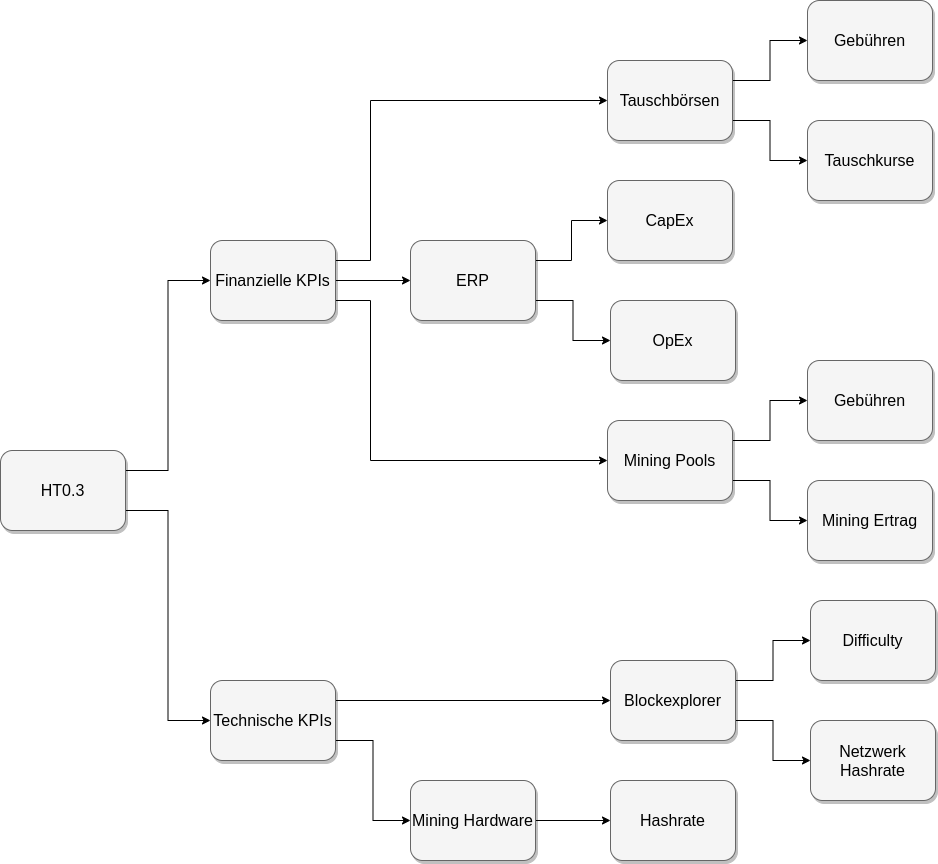
\includegraphics[width=0.7\textwidth]{ht03dataflow}
        \label{figure:ht03dataflow}
    \end{figure}

    \item \textbf{\ac{HT0.4}: }Die letzte Teilhypothese ist im Bereich der Personalplanung anzusiedeln und sagt aus, dass
    diese durch die Anwendung eines \ac{BI} Prozesses optimiert werden kann. Zur Beantwortung dieser Hypothese sind sowohl
    die technischen \acp{KPI} als auch die personellen \acp{KPI} von Bedeutung. Zu den technischen Indikatoren zählen Daten,
    wie die Ausfallzeiten und Informationen über die Art des Hardwaredefekts. Zu den personellen \acp{KPI} zählen wiederum Daten,
    wie Schichtpläne und Ausbildungen des Personals. Durch die Bereitstellung dieser Datenquellen ist es möglich, die
    durchschnittliche Dauer eines Reparaturvorgangs zu errechnen und anhand dessen die Personaldecke vor Ort realistisch
    einschätzen zu können. Nach Tabelle \ref{tbl:klassifizierunginternedaten} sind alle Daten konsistent und strukturiert,
    wodurch eine Verwendung dieser Daten in einem \ac{BI} möglich ist. Die \ac{ETL} Pipelines sind ohne weiteres realisierbar.
    Die technischen \acp{KPI} sind allerdings nur mit einer Verzögerung von fünf bis zehn Minuten zugänglich. Dies stellt jedoch
    für die Realisierbarkeit dieser Hypothese kein Problem dar, da andere Daten, wie beispielsweise neue Schichtpläne, nur einmal
    pro Monat aktualisiert werden und daher die Errechnung relevanter Ergebnisse nicht durch diese Verzögerung signifikant
    beeinflusst wird.

    \begin{figure}[H]
        \caption{Relevante KPIs, Datenquellen und Datentypen für Teilhypothese 4}
        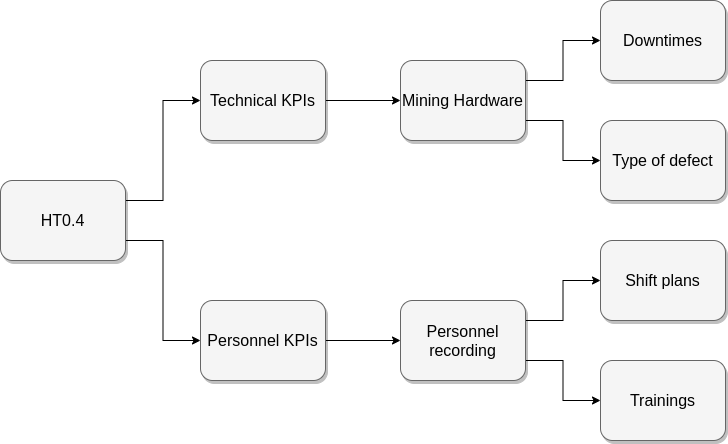
\includegraphics[width=0.55\textwidth]{ht04dataflow}
        \label{figure:ht04dataflow}
    \end{figure}
\end{itemize}

\subsubsection{Erforderliche Analyseverfahren innerhalb des Business Intelligence Prozesses} \label{toc:analyseverfahrenbi}

Um nun die Hypothesen final prüfen zu können, wird in diesem Kapitel geklärt, ob bereits etablierte Analyseprozesse dazu
ausreichen, die relevanten Daten für eine Hypothese so nutzbar zu machen, dass daraus Wissen generiert werden kann. Um dies
zu erreichen, werden die vorhandenen Analyseverfahren aus der Veröffentlichung von Bihani und Patil dem deskriptiven,
vorhersagenden oder präskriptiven Paradigma von \ac{BI} zugeordnet und analysiert, ob damit die einzelnen Teilhypothesen
beantwortet werden können:\footcite[Vgl.][S. 97ff]{bihani2014comparative}\footcite[Vgl.][Abb. 2]{bihani2014comparative}

\begin{itemize}
    \item \textbf{Deskriptive Analyse: }Diese Punkt beschreibt die Analyse der vergangenen und bereits erhobenen
    Daten. Die folgenden Analyseverfahren können für den deskriptiven Ansatz verwendet
    werden:\footcite[Vgl.][S. 97ff]{bihani2014comparative}
    \begin{itemize}
        \item \textbf{Faktorenanalyse: }Durch diese Form der Analyse werden unterliegende Strukturen in den Daten
        herausgefunden.\footcite[Vgl.][S. 97f]{bihani2014comparative} Dazu werden große multidimensionale Datensätze verwendet
        und diese zu kleineren Datensätze reduziert, die eine Aussagekraft haben. Diese Datensätze beinhalten dadurch
        grundlegende Faktoren, die die gemessenen großen Datensätze erklären
        können.\footcite[Vgl.][S. 97f]{bihani2014comparative} Solche Analysen sind unter anderem mittels \ac{OLAP} Systemen
        realisierbar. Für die Beantwortung der Teilhypothesen kann diese Form der Analyse verwendet werden. Es existieren
        in einem Data Warehouse, das die in Kapitel \ref{toc:klassifizierungderdaten} aufgeführten Daten beinhaltet, große
        Datensätze, wie beispielsweise die Hashrate der Mining Hardware oder auch Tauschkurse von \ac{BTC} in \ac{USD}. Auch
        ein Vergleich dieser Größen ist sinnvoll, wie beispielsweise von \ac{OpEx} und der Gesamthashrate eines Rechenzentrums.
        Aus diesen Gründen können die Faktorenanalyse und \ac{OLAP} Systeme für alle Teilhypothesen Sinn machen.
        \item \textbf{Clusteranalyse: }Dies ist ein Algorithmus der Ähnlichkeiten in Datensätzen identifizieren
        kann.\footcite[Vgl.][S. 98]{bihani2014comparative} Dadurch können Teilmengen der Datensätze als zusammenhängend
        klassifiziert werden. Unter den Überbegriff Clusteranalyse fallen viele Algorithmen, die aus dem Bereich "`Data Mining"'
        bekannt sind. Dazu zählt der "`K-Means-Algorithmus"' oder "`Nearest Neighbor"'.\footcite[Vgl.][S. 98]{bihani2014comparative}
        Das Ziel, große Datensätze durch Clustering Algorithmen zu unterteilen, bietet auch die Möglichkeit, die Strukturierung
        der Daten weiter erforschen zu können. Gerade bei den technischen \acp{KPI} ist daher diese Form der Analyse passend.
        Damit ist die Clusteranalyse für alle Teilhypothesen relevant und kann bei der Analyse von Hilfe sein. 
        \item \textbf{Diskriminanzfunktionsanalyse: }Die Analyse kann die Abweichung zweier gemessener Gruppen von Werten
        messen und dadurch bestimmen, ob eine Trennung existiert und wie stark diese
        ist.\footcite[Vgl.][S. 98]{bihani2014comparative} Die Anwendung dieser Analyse liegt klassischerweise im Verständnis
        von demographischen Faktoren beim Kauf von Produkten.\footcite[Vgl.][S. 98]{bihani2014comparative} Interessant ist diese
        Form der Analyse für die Interpretation der identischen \acp{KPI} aus verschiedenen Rechenzentren. Gerade die Analyse von
        Unterschieden von Daten zwischen Rechenzentren ermöglicht die Generierung von neuem Wissen und ist somit im Bereich
        \ac{BI} von unmittelbarer Relevanz. Die Anwendung der Diskriminanzfunktionsanalyse ist daher für alle Teilhypothesen
        sinnvoll, sobald mehr als ein Rechenzentrum betrachtet wird.
        \item \textbf{Strukturgleichungsmodell: }Dabei werden Abhängigkeiten zwischen Variablen gebildet und mittels linearen
        Gleichungssystemen geprüft, ob diese Beziehung tatsächlich existiert.\footcite[Vgl.][S. 98f]{bihani2014comparative} Als
        Ergebnis wird die Abhängigkeit bzw. Unabhängigkeit von dem vorgegebenen Modell
        festgestellt.\footcite[Vgl.][S. 98f]{bihani2014comparative}
        Gerade um mögliche Abhängigkeiten zwischen den einzelnen \acp{KPI} festzustellen, kann diese Form der Analyse verwendet
        werden. Ein einfaches Beispiel ist die Abhängigkeit von der Hashrate zum Ertrag durch den Mining Pool. Aufgrund dessen
        findet das Strukturgleichungsmodell auch bei den vorliegenden Teilhypothesen sinnvolle Anwendung.
    \end{itemize}
    Zusammenfassend ist feststellbar, dass es eine Vielzahl von verschiedenen Möglichkeiten gibt, die vorliegenden Daten zu
    analysieren und dadurch Wissen für die Stakeholder generieren zu können. Mit Hilfe der vorliegenden Analyseformen ist
    ein deskriptiver \ac{BI} Prozess mit den Teilhypothesen durchführbar.

    \item \textbf{Vorhersagende Analyse: }Bei diesem Paradigma werden Modelle zur Vorhersage mittels verschiedener Werkzeuge
    gebildet. Viele dieser Werkzeuge kommen aus dem Bereich der Statistik und des maschinellen
    Lernens.\footcite[Vgl.][Abb. 1]{bihani2014comparative} Folgende Formen der Analyse kommen zusätzlich zu den bereits
    genannten Formen hinzu:
    \begin{itemize}
        \item \textbf{Regressionsanalyse: }Bei dieser Form der Analyse wird die Abhängigkeit einer Variable von einer oder
        mehreren Variablen geprüft.\footcite[Vgl.][S. 97f]{bihani2014comparative} Dabei gibt es mehrere Formen, wie die lineare
        oder die logistische Regression verwendet werden kann. Diese Analyse kann bei der Prognose der Profitabilität
        oder von Marktanteilen sehr gut verwendet werden.\footcite[Vgl.][S. 99]{bihani2014comparative} Aus diesem Grund kann
        diese auch für die zu prüfenden Teilhypothesen von Relevanz sein. Eine Anwendung der
        Regressionsanalyse ist die Prognose des Wertes von Bitcoins.\footcite[Vgl.][S. 19]{ibrahim2020bitcoin} Prinzipiell
        ist eine Vorhersage mit Hilfe dieser Mechanismen gut möglich. Ende 2020 sind Faktoren, wie Social Media dazugekommen,
        die diese Form der Analyse deutlich erschweren.\footcite[Vgl.][]{forbes2021musk} Demzufolge kann die Regressionsanalyse eine
        Methodik sein, um Kurse vorhersagen zu können, muss allerdings um weitere Analysemodelle erweitert werden, um ein gutes
        Gesamtbild zu erhalten. 
        \item \textbf{Stochastische Analyse: }Es ist möglich Vorhersagemodelle auf Basis von stochastischen Modellen zu
        simulieren. Ein bekanntes Beispiel für eine stochastische Analyse ist die "`Monte-Carlo-Simulation"'. Sie kann
        beispielsweise verwendet werden, um Preisentwicklungen und Entwicklungen der Gesamthashrate von Bitcoin für die Zukunft
        einschätzen zu
        können.\footcite[Vgl.][S. 28]{cocco2016modeling}\footcite[Vgl.][]{appendix:mcszenarien}\footcite[Vgl.][]{appendix:mcpreis}\footcite[Vgl.][]{appendix:mchashrate}
        Auch bei dieser Form der Simulation, die am 06.11.2020 angefertigt wurde ist feststellbar, dass diese die Entwicklungen
        des Bitcoin Kurses Anfang 2021 nicht vorhersagen konnte.\footcite[Vgl.][]{appendix:btcusd} Daher ist dieses Analysemodell für sich nicht direkt aussagekräftig,
        sondern muss durch weitere Modellierungen unterstützt werden.
    \end{itemize}

    Letztendlich kann festgehalten werden, dass der Bitcoin Preis nur bedingt vorhergesagt werden kann, da einige Einflussfaktoren, wie
    beispielsweise Social Media, nicht vorhergesagt werden können und sich mathematischen Möglichkeiten der Analyse weitestgehend entziehen.\footcite[Vgl.][]{forbes2021musk}\footcite[Vgl.][S. 325]{badertscher2017bitcoin}
    Generell ist dies allerdings kein ausschließliches Problem, das bei Bitcoin auftritt. Bei den klassischen Märkten ist das gleiche
    Problem bemerkbar. Aufgrund der hohen Volatilität des Bitcoin Kurses ist es in diesem Fall jedoch auffälliger.
    Andere \acp{KPI}, wie beispielsweise \ac{OpEx} Kosten oder technische \acp{KPI}, sind im Gegensatz dazu prognostizierbar, da diese
    wenig bis keine Schwankungen unterliegen und somit die Ergebnisse der deskriptiven Analyse unter diesem Paradigma weiterhin
    verwendet werden können. 
    Demnach ist feststellbar, dass \ac{HT0.2} und \ac{HT0.4} für Vorhersagemodelle geeignet sind, da diese ausschließlich \acp{KPI} verwendet,
    die in ausreichender Qualität simuliert werden können. Bei \ac{HT0.1} und \ac{HT0.3} können auch vorhersagende Modelle angewendet werden,
    wobei eine Limitation durch die Vorhersage des Bitcoin Kurses festgestellt werden kann. Dies kann durch eine geeignete Kombination der
    Analysemodelle verbessert werden. Falls es möglich ist, die unstrukturierten und inkonsistenten Daten aus Social Media Plattformen passend zu analysieren,
    sollten diese in die Vorhersagemodellierungen integriert werden. Um einen möglichst guten Eindruck des \ac{BTC} Kurses zu erhalten,
    ist es wichtig mit Echtzeitverarbeitung dieser Daten zu arbeiten.
    \item \textbf{Präskriptive Analyse: }Diese ist die höchste Stufe, die mit Hilfe von \ac{BI} Prozessen erreichbar ist. Dabei werden
    nicht nur Entscheidungshilfen dem Management zur Verfügung gestellt sondern es werden direkt Entscheidungen dem Management durch
    das System empfohlen. Die Analyse der Hypothese läuft ähnlich zu dem Punkt der Vorhersagemodelle, da diese Stufe von \ac{BI} auch
    auf diesen Modellen beruht. Demgemäß ist das Ergebnis dieser Analyse identisch mit der vorherigen und \ac{HT0.2} und \ac{HT0.4} sind in dieser 
    Stufe realisierbar. Wie bei dem vorherigen Punkt bereits aufgezeigt, haben die beiden anderen Hypothesen Limitationen, die aus
    der schlechten Vorhersagbarkeit des Bitcoin Kurses stammen. Eine Möglichkeit, dass die beiden Teilhypothesen doch für die
    präskriptive Analyse geeignet sind, wäre die Errechnung verschiedener Szenarien des Bitcoin Kurses und damit die Errechnung
    verschiedener Mining Erträge. Solche Vorhersagemodelle existieren innerbetrieblich bereits durch die Monte-Carlo-Simulation der Hashrate
    und des Bitcoin Kurses.\footcite[Vgl.][]{appendix:mcpreis}\footcite[Vgl.][]{appendix:mchashrate}
    Da die Antwort auf die Umsetzbarkeit eines solchen Systems nur schwer im Zuge dieser Argumenation gegeben werden kann, wird
    dies in der Fallstudie in Kapitel \ref{toc:planungeinesbiprozessesfuereinminingrechenzentrum} genauer betrachtet.
\end{itemize}

Außerhalb dieser Auflistung existieren noch zusätzliche Analyseformen, wie beispielsweise die Verbundsanalyse.\footcite[Vgl.][S. 97]{bihani2014comparative}
Diese findet beispielsweise bei Analyse des Kaufverhaltens von Kunden Anwendung. Aufgrund der nicht gefundenen Relevanz für den Anwendungsfall von Kryptomining
Rechenzentren wird diese Form nicht weiter in Betracht gezogen.

In Tabelle \ref{tbl:hypothesenanalyse} sind die Ergebnisse der vorhergehenden Analyse zusammenfassend visualisiert.

\begin{table}[H]
    \caption{Mögliche Analyseformen der Hypothesen}
    \label{tbl:hypothesenanalyse}
    \begin{tabularx}{\textwidth}[ht]{X||c|c|c|c}
        & \ac{HT0.1} & \ac{HT0.2} & \ac{HT0.3} & \ac{HT0.4}  \\
        \hline\hline
        Deskriptive Analyse & \checkmark & \checkmark & \checkmark & \checkmark \\
        \hline
        Vorhersagende Analyse & (\checkmark) & \checkmark & (\checkmark) & \checkmark \\
        \hline
        Präskriptive Analyse & (\checkmark) & \checkmark & (\checkmark) & \checkmark \\
    \end{tabularx}
    \begin{tablenotes}
        \item \hspace{1mm}\checkmark\hspace{10mm} Durchführbar
        \item (\checkmark)\hspace{8.5mm} Unter den beschriebenen Limitationen durchführbar
    \end{tablenotes}
\end{table}

Mit Abschluss dieses Kapitels ist geklärt, ob die Einführung eines \ac{BI} Prozesses für die jeweiligen Teilhypothesen möglich ist.
Im nächsten Kapitel werden schlussendlich die Ergebnisse der vier Teilhypothesen verwendet, um eine erste Aussage über die Haupthypothese
zu erhalten und damit die Forschungslücke, die diese Arbeit schließen soll, erstmalig zu beantworten.

\subsection{Zusammenfassende Betrachtung} \label{toc:zusammenfassendebetrachtung}

Nachdem in Kapitel \ref{toc:analyseverfahrenbi} die Prüfung der einzelnen Teilhypothesen vorgenommen wurde,
wird in diesem Teil dieses Wissen verwendet, um eine Aussage über die Haupthypothese zu erhalten.

Es existieren vier Stufen, die bei der Analyse von Daten erreicht werden können. Diese Stufen finden sich in Abbildung
\ref{figure:levelofanalysis}. Es wird folgend die Relevanz der Haupthypothese in den einzelnen Stufen evaluiert
und anhand dessen die Aussagen der Teilhypothesen auf die Haupthypothese projiziert. Die Stufen teilen sich
folgendermaßen auf:\footcite[Vgl.][Abb. 2]{bihani2014comparative}

\begin{figure}[H]
    \caption{Stufen der Datenanalyse}
    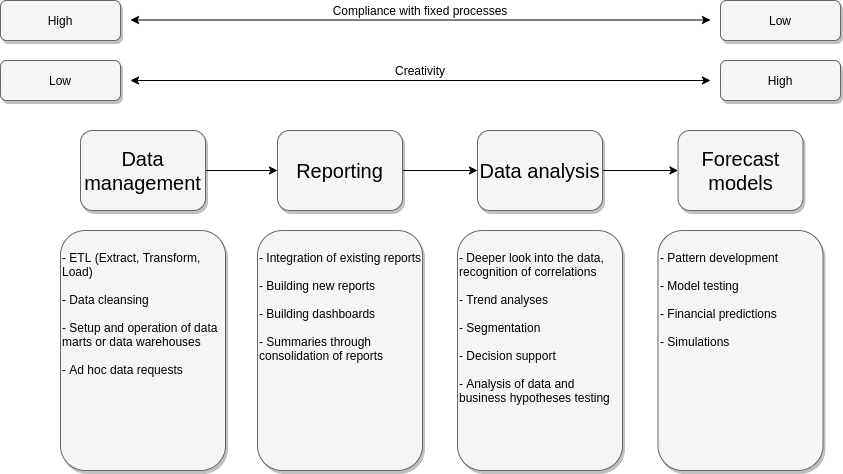
\includegraphics[width=0.8\textwidth]{levelofanalytics}
    \label{figure:levelofanalysis}
    \\
    \cite[Quelle: In Anlehnung an][Abb. 2]{bihani2014comparative}
\end{figure}

\begin{itemize}
    \item \textbf{Management der Daten: }Das Management der verschiedenen Daten ist ohne weiteres möglich. Alle relevanten
    Daten sind verfügbar und können in ein Data Warehouse eingespeist werden. Diese Analyse findet sich in Kapitel
    \ref{toc:internedatenquellen} und deren Zusammenfassungen in Tabelle \ref{tbl:klassifizierunginternedaten} und
    \ref{tbl:klassifizierungexternedaten}. Das Management der Daten ist auch für die Haupthypothese von unmittelbarer
    Wichtigkeit, da dies die Grundlagen für die Optimierung von Kryptomining Rechenzentren legt. Da bei allen Teilhypothesen
    das Management der Daten möglich ist, ist es das auch für die Haupthypothese. Es ist feststellbar, dass die erste
    Stufe ohne Probleme erreichbar ist.
    \item \textbf{Berichtswesen: }Die zweite Stufe der Verwendung von Daten ist die Errichtung eines Berichtwesens. Ein Berichtswesen
    verwendet die existierenden Daten der Vergangenheit, um für die Stakeholder des \ac{BI} Prozesses passende Berichte zu generieren.
    In diesem Fall sind dies Berichte, die die Teilhypothesen abdecken und damit personeller, technischer oder finanzieller
    Natur sind. Da diese
    Stufe deskriptiv ist, ist auch dies nach Tabelle \ref{tbl:hypothesenanalyse} für alle vier Teilhypothesen
    möglich. Daher ist möglich, das Berichtswesen für die Aussagen der Haupthypothese anzuwenden. Gerade diese Stufe ist für
    die Erreichung der zentralen Aussage der Haupthypothese ("`finanzielle Optimierung"') zentral, weil dies die Grundlage
    für die Optimierung eines Kryptomining Rechenzentrums legt.
    \item \textbf{Analyse der Daten: }Im dritten Schritt werden die Daten tiefer analysiert, um mehr Zusammenhänge zwischen den
    Daten feststellen zu können und damit mehr Wissen generieren zu können, was letztendlich für die Optimierung von Rechenzentren
    weiterhin verwendet werden kann. Daher ist auch die Haupthypothese in dieser Stufe anzutreffen. Dabei werden die bereits
    vorhandenen Daten verwendet, um Aussagen und Entscheidungshilfen zu generieren. Zu dieser Stufe gehören die
    bereits in Kapitel \ref{toc:analyseverfahrenbi} genannten Analyseverfahren, die Unterstützung bei Entscheidungen und auch
    die Analyse von geschäftlichen Hypothesen.
    Da diese Stufe wieder auf den vorhandenen Daten beruht und keine direkten Vorhersagen tätigt, ist diese
    Stufe für alle Teilhypothesen zu erreichen. Daher ist feststellbar, dass die Haupthypothese ebenfalls für diese Stufe positiv beantwortbar ist.
    Erst ab dieser Stufe ist der eigentliche \ac{BI} Prozess erreicht, weil erst ab diesem Zeitpunkt die Unterstützung
    bei Entscheidungen mit ins Spiel kommt. Deswegen ist eine finanzielle Optimierung von Kryptomining Rechenzentren mittels
    \ac{BI} grundsätzlich möglich.
    \item \textbf{Vorhersagemodelle: }Die letzte Stufe ist die Bildung von Vorhersagemodellen. Das ist der vorhersagende Teil von
    \ac{BI} und legt die Grundlagen für präskriptive \ac{BI} Systeme. Diese Stufe ist für \ac{HT0.2} und \ac{HT0.4} ohne Probleme
    zu erreichen. Die Probleme sind bei \ac{HT0.1} und \ac{HT0.3} ausschließlich auf die schlechte Vorhersagbarkeit von Bitcoin
    Tauschkursen zurückzuführen. Falls es in diesem Bereich Verbesserungen gibt, kann auch diese Stufe erreichbar sein.
    Mögliche Ansätze zur Verbesserung werden in Kapitel \ref{toc:planungeinesbiprozessesfuereinminingrechenzentrum}
    evaluiert und letztendlich zur Einschätzung der Haupthypothese hinzugefügt. In diesem Zuge dieser Argumenation ist noch
    keine finale Antwort auf die Haupthypothese an dieser Stelle zu finden.
\end{itemize}

Im nächsten Kapitel werden die Aussagen aus diesem Teil durch eine Fallstudie evaluiert, um belastbare Aussagen über
die Hypothesen zu bekommen und diese durch zwei Methodiken zu stützen und zu erweitern. Es wird dabei der Fokus
auf die Prüfung der Teilhypothesen in Bezug auf die Vorhersagemodelle gelegt, um diesen offenen Teil
letztendlich beantworten zu können.

\newpage
\section{Planning of a business intelligence process for a mining data center} \label{toc:planungeinesbiprozessesfuereinminingrechenzentrum}

The following chapter evaluates whether an \ac{BI} process is operationally feasible under the conditions developed in the previous chapter.
For this examination exist among other things two approaches, which are described in the publication
"Business Intelligence Stategy" by John Boyer et al:\footcite[Cf.][p. 102]{boyer2010business}

\begin{itemize}
    \item \textbf{Stakeholder analysis: } In chapter \ref{toc:stakeholderanalyse} the stakeholders of the concerned
    \ac{BI} Process are identified. This makes it possible to identify technological approaches to realization
    and to analyze whether this process will have sufficient support within the company. This support
    depends primarily on how many stakeholders benefit from the added value of a \ac{BI} process.
    Based on this, in chapter \ref{toc:datenpraesentation}
    identifies the appropriate forms of data presentation.\footcite[Cf.][p. 102]{boyer2010business}
    \item \textbf{Technological environment:}The technological environment within the business is analyzed.
    This allows components to be identified that already exist and only need to be integrated.\footcite[Cf.][p. 102]{boyer2010business} Additionally
    the argumentation from chapter \ref{toc:ansatzmoeglichkeitenfuerbusinessintelligence} can be extended or supported with it.
    As technological basis for the realization the Google Cloud is considered, since this is used within the
    Genesis Group is strongly used.
\end{itemize}

To obtain meaningful results on these two points, a small case study is designed in chap.
\ref{toc:fallstudiendesign} is designed so that operational feasibility can be tested. Towards the end of the chapter, the
results from this study are briefly summarized and evaluated. A critical evaluation of the entire argumentation takes place
in the conclusion of this thesis.

\subsection{Case study design and methodology} \label{toc:fallstudiendesign}

In this part, the basic structure of the case study is described. For the design of the case study the approach of
Göthlich.\footcite[Cf.][]{gothlich2003fallstudien} The approach is summarized in Fig.
\ref{figure:casestudydesign}.

\begin{figure}[H]
    \caption{Case study design and methodology}
    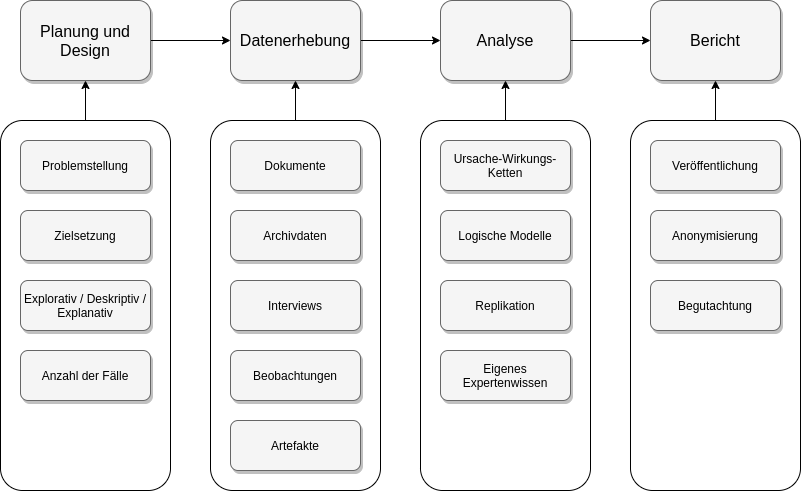
\includegraphics[width=0.8\textwidth]{casestudydesign}
    \label{figure:casestudydesign}
    \\
    \cite[Source: Based on][pp. 8]{gothlich2003fallstudien}
\end{figure}

In the following, the individual steps are described and thereby the design is
defined:\footcite[Cf.][pp. 8]{gothlich2003fallstudien}
\begin{itemize}
    \item \textbf{Planning and design: }The first step is to state the problem and the objectives to be covered by the case study.
    The problem statement is already described in chapter \ref{toc:motivation} and \ref{toc:hypothesenundabgrenzungderarbeit}.
    The goal of this case study is to answer the hypotheses in chapter \ref{toc:ansatzmoeglichkeitenfuerbusinessintelligence}
    by examining its operational feasibility. It is to be increased the resilience of the statements of this work, in that
    planning an application in practice on the basis of the theoretical analysis.
    Therefore, the research objective in the study is exploratory in nature.\footcite[Cf.][p. 8]{gothlich2003fallstudien}
    This case study is conducted once in this form ("single case"). This eliminates any possible replication of this study.\footcite[Cf.][pp. 8]{gothlich2003fallstudien}
    \item \textbf{Data collection: }This step defines the data sources available for the case study. In addition to the
    data sources described in chapter \ref{toc:klassifizierungderdaten}, additional internal documents of the Genesis
    Group are available. These can be found in the appendix to this thesis. Therefore, the case study is based on documents and artifacts.\footcite[Cf.][Table 1 ]{gothlich2003fallstudien}
    \item \textbf{Analysis: }In the course of the analysis, a model for an exemplary \ac{BI} Process,
    which can be applied within the Genesis Group, will be created. On the basis of this it is examined whether the introduction is possible and thereby the
    hypotheses of this thesis can be supported. For this purpose, "cause-effect chains" and logical models are used.\footcite[Cf.][p. 11]{gothlich2003fallstudien}
    In both of these analytical models, strong reference is made to an operational environment.
    \item \textbf{Report: }The final step deals with the publication of this case study. Since this case study takes place in the context
    of this thesis, a publication is already planned. A peer review is nevertheless useful and will be done in the course of
    of the subsequent internal evaluation.
\end{itemize}

In the following, a stakeholder analysis is performed using the Genesis Group as an example. With the help of the results of this analysis and the additional
theoretical knowledge from this thesis, an exemplary \ac{BI} process will be created in chapter \ref{toc:planungdesbiprozesses} and will
finally be checked for its feasibility in chapter \ref{toc:abschliessendebewertung}.

\subsection{Stakeholder analysis for an internal business intelligence process} \label{toc:stakeholderanalyse}

The following stakeholder analysis is primarily based on the publication "A Stakeholder Model of Business
Intelligence" by Claire A. Simmers.\footcite[Cf.][]{simmers2004stakeholder} This work deals with
stakeholder analysis in the field of \ac{BI} and is used for the present analysis. Based on
Figure 14.2 in this publication, the stakeholder analysis is operated and thus the individual persons or groups are identified,
who have an interest in the successful implementation of a \ac{BI} Process.\footcite[Cf.][Fig. 14.2]{simmers2004stakeholder}

The following stakeholders can be identified for cryptomining data center optimization in the cloud mining environment:\footcite[Cf.][Fig. 14.2]{simmers2004stakeholder}\footcite[Cf.][p. 52]{reed2009s}

\begin{itemize}
    \item \textbf{Company owners: }The owners of Genesis Group are responsible for the strategic decisions and
    have an interest in the successful implementation
    of such a \ac{BI} Process. This may include reasons such as improving mining revenue, advantages in the cloud mining market
    through increased data center efficiency, and decision support regarding the new or expansion of mining
    data centers. Therefore, \ac{HT0.1} and \ac{HT0.3} are mainly relevant to these individuals.
    \item \textbf{Employees: }Another relevant group are the employees of the Genesis Group. These benefit
    by the introduction of \ac{BI} especially with regard to time savings, process optimization and
    decision support (Cf. chapter \ref{toc:strategischermehrwert}). This group can be divided into the following subgroups:
    \begin{itemize}
        \item Business management: This group has significant interest in the decision support that a \ac{BI} Process
        provides. Tactical decisions that affect data center operations are made by this group.
        For this reason, management has an interest in an accurate representation of a data center's cash flow, which is
        is reviewed in \ac{HT0.3}.
        \item Management of the data centers: This group manages the existing data centers and can be found in the area of operational decisions.
        It has an interest in operating the most efficient hardware possible (\ac{HT0.2}),
        the cash flow of a data center (\ac{HT0.3}) and the optimization of the staffing of a mining data center
        (\ac{HT0.4}).
        \item Controlling: The controlling department is responsible for the financial monitoring of the data centers. Therefore, this
        group of people has direct interest in a fast and correct access to the financial data from which
        ultimately the cash flow can be calculated (\ac{HT0.3}).
        \item IT: The technical departments are primarily responsible for maintaining and operating the existing hardware.
        Therefore, they mainly need technical \acp{KPI}, which is covered by \ac{HT0.2}. Due to the availability
        of this data, the efficiency of the hardware can be better estimated and possible improvements identified.
    \end{itemize}
    \item \textbf{Investors: }Investors are interested in data, facts, and predictions that are
    are comprehensible and transparent. For these reasons, the group of investors is also one of the stakeholders in a \ac{BI} process,
    since it fulfills exactly these requirements of these stakeholders for an investment object.
    \item \textbf{Suppliers: }Suppliers, such as hardware suppliers or energy providers, are stakeholders of an
    \ac{BI} Process. Their available data is used in such a process, among other things, to optimize the company's purchasing activities.
    By means of \ac{BI}, it is possible, for example, to identify the appropriate hardware for a mining data center
    or to support the selection of the energy supplier.
    \item \textbf{Customers: }Furthermore, the customers who have a cloud mining contract with Genesis Group are stakeholders. These
    have an interest, analogous to the company owners, in obtaining the highest possible and at the same time stable revenue from mining. 
    Therefore, this group has an interest in using the best possible hardware, software and mining pools.
\end{itemize}

The relavant stakeholders from the analysis are summarized visualized in Figure \ref{figure:internalstakeholder}.

\begin{figure}[H]
    \caption{Stakeholders and their main interest in an internal \ac{BI} process}
    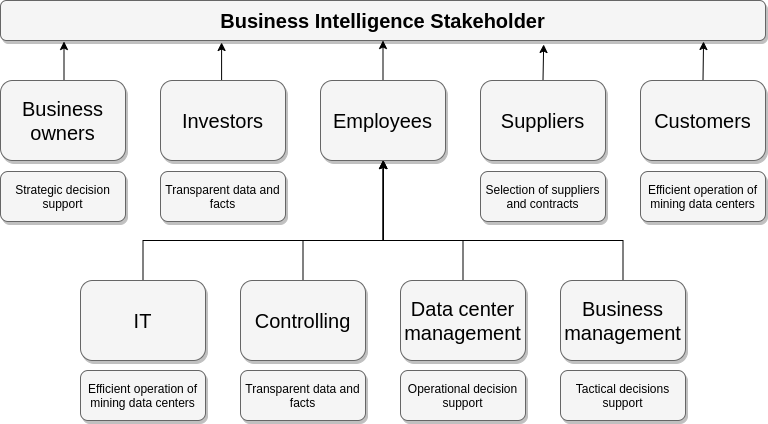
\includegraphics[width=0.8\textwidth]{internalstakeholder}
    \label{figure:internalstakeholder}
\end{figure}

Other groups of stakeholders exist but have no influence on the \ac{BI} evaluation.
These include political groups, governments, and the community.\footcite[Cf.][Fig. 14.2]{simmers2004stakeholder}

\subsection{Planning of the Business Intelligence process} \label{toc:planungdesbiprozesses}

In the following part, an exemplary \ac{BI} Process in an operational environment is planned. The company for which this process is
is planned is the Genesis Group and has already been described in chapter \ref{toc:motivation}. For the planning
the conclusions from chapter \ref{toc:ansatzmoeglichkeitenfuerbusinessintelligence} are used. Within the Genesis Group
the Google Cloud is used for the IT infrastructure, which is why suitable sample products from this cloud are identified in the following
chapters.\footcite[Cf.][]{googlecloud2021dw} Analogous to a \ac{BI} Process, the following study is divided into the steps of data acquisition
(chapter \ref{toc:datenhaltung}), data analysis (chapter \ref{toc:datenanalyse}), and data presentation (chapter \ref{toc:datenpraesentation}).
At the end, there is an evaluation of the study, which includes the argumentation of the sub-hypotheses from chapter
\ref{toc:ansatzmoeglichkeitenfuerbusinessintelligence} and supplements it if necessary.


\subsubsection{Data acquisition} \label{toc:datenhaltung}

Als Datenquellen werden die in Kapitel \ref{toc:klassifizierungderdaten} aufgezeigten Schnittstellen und Systeme verwendet.
Wie aus Tabelle \ref{tbl:klassifizierunginternedaten} und \ref{tbl:klassifizierungexternedaten} hervorgeht, sind alle Datenquellen für die
Verwendung innerhalb eines \ac{BI} geeignet und können daher in dementsprechenden \ac{ETL} Pipelines verwendet werden.
Eine Möglichkeit \ac{ETL} Pipelines in der Cloud errichten zu können, ist die Verwendung des "`Cloud Data Fusion"'
Dienstes.\footcite[Cf.][]{googlecloud2021dw} Dieser ist auf den Aufbau solcher Pipelines spezialisiert und bietet zudem Schnittstellen
zu einem Data Warehouse in der Cloud an. Das Data Warehouse an sich wird über den "`Big Query"' Dienst realisiert.\footcite[Cf.][]{googlecloud2021dw}
Dieses Warehouse ist der zentrale Ort, an dem alle relevanten Daten für die Analysephase des \ac{BI} Prozesses gespeichert werden und
ist daher zusammen mit den \ac{ETL} Pipelines für den Aufbau von \ac{BI} nicht wegzudenken.\footcite[Cf.][pp. 105]{loshin2012business}
Das Data Warehouse wird über den "`Cloud Data Fusion"' Dienst befüllt. Nach diesem Schritt sind alle benötigten Daten intern
im eigenen Data Warehouse verfügbar. Deshalb ist anzunehmen,
dass die Erhebung und die Beschaffung von Daten unter Zuhilfenahme der Google Cloud möglich ist und die betriebliche
Umsetzung für diesen Schritt gegeben ist.

The interfaces and systems shown in chapter \ref{toc:klassifizierungderdaten} are used as data sources.
As shown in table \ref{tbl:klassifizierunginternedaten} and \ref{tbl:klassifizierungexternedaten}, all data sources are suitable for the
use within \ac{BI} and can therefore be used in corresponding \ac{ETL} pipelines.
One way to build \ac{ETL} pipelines in the cloud is to use the "Data Fusion"
service.\footcite[Cf.][]{googlecloud2021dw} This specializes in setting up such pipelines and also provides interfaces
to a data warehouse in the cloud. The data warehouse itself is realized via the "Big Query" service.\footcite[Cf.][]{googlecloud2021dw}
This warehouse is the central location where all relevant data for the analysis phase of the \ac{BI} process is stored and
is therefore indispensable together with the \ac{ETL} pipelines for building a \ac{BI} process.\footcite[Cf.][pp. 105]{loshin2012business}
The data warehouse is populated via the "Cloud Data Fusion" service. After this step, all required data is available internally
in the own data warehouse. Therefore, it can be assumed
that the collection and the acquisition of data with the help of the Google Cloud is possible and that the operational implementation for this step is given.

\subsubsection{Data analysis} \label{toc:datenanalyse}

For the analysis of the data, which is now available in a data warehouse, the analysis procedures are used, which are described in
chapter \ref{toc:analyseverfahrenbi}. In the Google Cloud, there are several possible products for the realization of these procedures.\footcite[Cf.][]{googlecloud2021dw}
These include the products "Looker", which is a \ac{OLAP} platform for \ac{BI},
the "Dataflow" service, which analyzes datasets in real time as well as in batches, and "Dataproc", which has the ability
among other things, to run Apache Spark.\footcite[Cf.][]{googlecloud2021dw} All of these tools are sufficient to complete the analysis phase
of a \ac{BI} process. 

The result from chapter \ref{toc:zusammenfassendebetrachtung} was that the implementation of a \ac{BI} process is possible, but there are
difficulties in predicting the Bitcoin exchange rate. This problem is not directly limited to Bitcoin
itself, but is the case for predicting any exchange rate. 
One way to work with predictive models is not to predict a concrete
price, but to build different scenarios that include possible reactions and decisions of the management.\footcite[Cf.][]{appendix:mcpreis}
An appropriate way to do this is to use stochastic models, especially Monte Carlo simulations.\footcite[Cf.][p. 28]{cocco2016modeling}
These are already used for scenario building in the Genesis Group. The Monte Carlo simulation at hand was
made on 06.11.2020.\footcite[Cf.][]{appendix:mcpreis} When comparing to real data from this time, it is noticeable that this form of simulation is suitable
for predictive models for the near future (< 1 month).\footcite[Cf.][]{appendix:btcusd} The further events were largely determined by social media
and therefore could not be mapped within the scope of this simulation.
This form of simulation gives the possibility
to calculate and statistically evaluate any number of possible price developments.
evaluation.\footcite[Cf.][]{appendix:mcpreis}\footcite[Cf.][]{appendix:mcszenarien} This results in multiple
scenarios that imply different management responses. The initial values for such an analysis
are provided by the data warehouse. The results
are in turn entered into the data warehouse and are thus accessible to other analysis procedures. However, as already
in chapter \ref{toc:ansatzmoeglichkeitenfuerbusinessintelligence}, social media platforms, for example, have a major influence on the
development of the Bitcoin price. Such developments cannot be represented directly with stochastic models.
Here again, real-time processing of the data is important so that the stakeholders already described can react directly.
In addition to the development of the Bitcoin price, it is possible through a Monte-Carlo simulation to show the development of the entire
network hashrate of the Bitcoin network.\footcite[Cf.][]{appendix:mchashrate}

It can be seen that by switching from strict predictive models to coarser scenario building,
the predictive aspect of \ac{BI} can be implemented. Also, for sub-hypotheses one and three, predictive and
prescriptive \ac{BI} is possible. Operational feasibility is given.

\subsubsection{Data presentation} \label{toc:datenpraesentation}

This part deals with the process of how the knowledge generated by the appropriate analysis of the data is now made available to the
relevant stakeholders in the correct manner, thereby achieving the goal of decision support.
For this purpose, the stakeholders from chapter \ref{toc:stakeholderanalyse} are considered in the following. There are several
ways in which knowledge can be made available to these individuals and groups:\footcite[Cf.][Chap. 19]{loshin2012business}
\begin{itemize}
    \item \textbf{Reporting: }This is the simplest form of presentation. In this case
    static report templates are configured, from which regular reports are automatically generated and made available to the stakeholders.\footcite[Cf.][p. 305]{loshin2012business}
    Examples of such reports in the context of this work include reports on mining downtime
    or monthly summaries of the financial situation of data centers. The generation of such reports can be done in
    Google Cloud via the "Cloud Scheduler".\footcite[Cf.][]{googlecloud2021scheduler} The relevant stakeholders can be provided with the reports accordingly.
    \item \textbf{\ac{OLAP} and Ad-Hoc Searches: }In this form of presentation, a \ac{OLAP} system is used to create one's own search queries
    and thus generate tailored knowledge.\footcite[Cf.][pp. 308]{loshin2012business}
    These search queries can be created spontaneously (ad-hoc) through the \ac{OLAP} system
    and results are provided directly to the stakeholder. Examples include queries that concern the new construction or
    expansion of mining data centers. An example of such a system is the "Looker" service of the
    Google Cloud.\footcite[Cf.][]{googlecloud2021dw}
    \item \textbf{Dashboards: }Another method of making analytics knowledge available to stakeholders
    is the use of dashboards. These dashboards
    can be accessed online and present data obtained through the underlying software.\footcite[Cf.][pp. 314]{loshin2012business} Especially for
    technical \acp{KPI}, such as the display of hashrates or power consumption of the hardware, this form of
    visualization is used. Furthermore, stakeholders are able to create their own dashboards.\footcite[Cf.][pp. 314]{loshin2012business}
    A common application for creating dashboards is "Grafana".\footnote{https://grafana.com}
    \item \textbf{Alerting: }This method proactively sends notifications and alerts to
    relevant stakeholders.\footcite[Cf.][pp. 311]{loshin2012business} This enables them to respond to changing circumstances with only a small time lag. For example,
    the complete failure of a data center or deviations of reality from the forecast models are cases in which an alert can make sense.
    Such alerts can then be delivered to the relevant stakeholders via mail or instant messenger.\footcite[Cf.][pp. 311]{loshin2012business}
    A service that allows the creation of such alerts is the "Pub/Sub" service.\footcite[Cf.][]{googlecloud2021dw} For the sending of alerts
    monitoring systems, such as "Prometheus", can be used.\footnote{https://prometheus.io}
\end{itemize}

All these forms of presentation can easily be carried out in-house. Therefore, there are no internal obstacles
to the implementation of an \ac{BI} process.

\subsection{Final evaluation} \label{toc:abschliessendebewertung}

In chapter \ref{toc:planungdesbiprozesses}, a small case study discussed whether it is possible to implement a \ac{BI} Process,
as it was shown in chapter \ref{toc:ansatzmoeglichkeitenfuerbusinessintelligence}.
In order to achieve this, the three main steps of an \ac{BI} process, data acquisition, analysis and presentation, were discussed individually
and possible technical solutions were demonstrated using the Google Cloud as an example.

In summary, it can be stated that there are no obstacles that contradict the introduction of an \ac{BI} process.
In addition to the argumentation from chapter \ref{toc:ansatzmoeglichkeitenfuerbusinessintelligence}, it is possible that the \ac{BI} Process
is feasible up to the prescriptive paradigm (Cf. Table \ref{tbl:hypothesenanalyse2}). Therefore, it is possible without restriction that all sub-hypotheses
can be mapped in such a process. Thus, in conclusion it is possible to say that the main hypothesis of this work can be confirmed.
By means of \ac{BI} it is possible that cryptomining data centers can be optimized financially.

\begin{table}[H]
    \caption{Result of the feasibility of a business intelligence process}
    \label{tbl:hypothesenanalyse2}
    \begin{tabularx}{\textwidth}[ht]{X||c|c|c|c}
         & \ac{HT0.1} & \ac{HT0.2} & \ac{HT0.3} & \ac{HT0.4}  \\
        \hline\hline
        Descriptive analysis & \checkmark & \checkmark & \checkmark & \checkmark \\
        \hline
        Predictive analysis & \checkmark & \checkmark & \checkmark & \checkmark \\
        \hline
        Prescriptive analysis & \checkmark & \checkmark & \checkmark & \checkmark \\
    \end{tabularx}
\end{table}

An example \ac{BI} Process for the Genesis Group example may look like the one shown in Figure \ref{figure:internalbiprocess}.

\begin{figure}[H]
    \caption{Design of a BI process within the Genesis Group}
    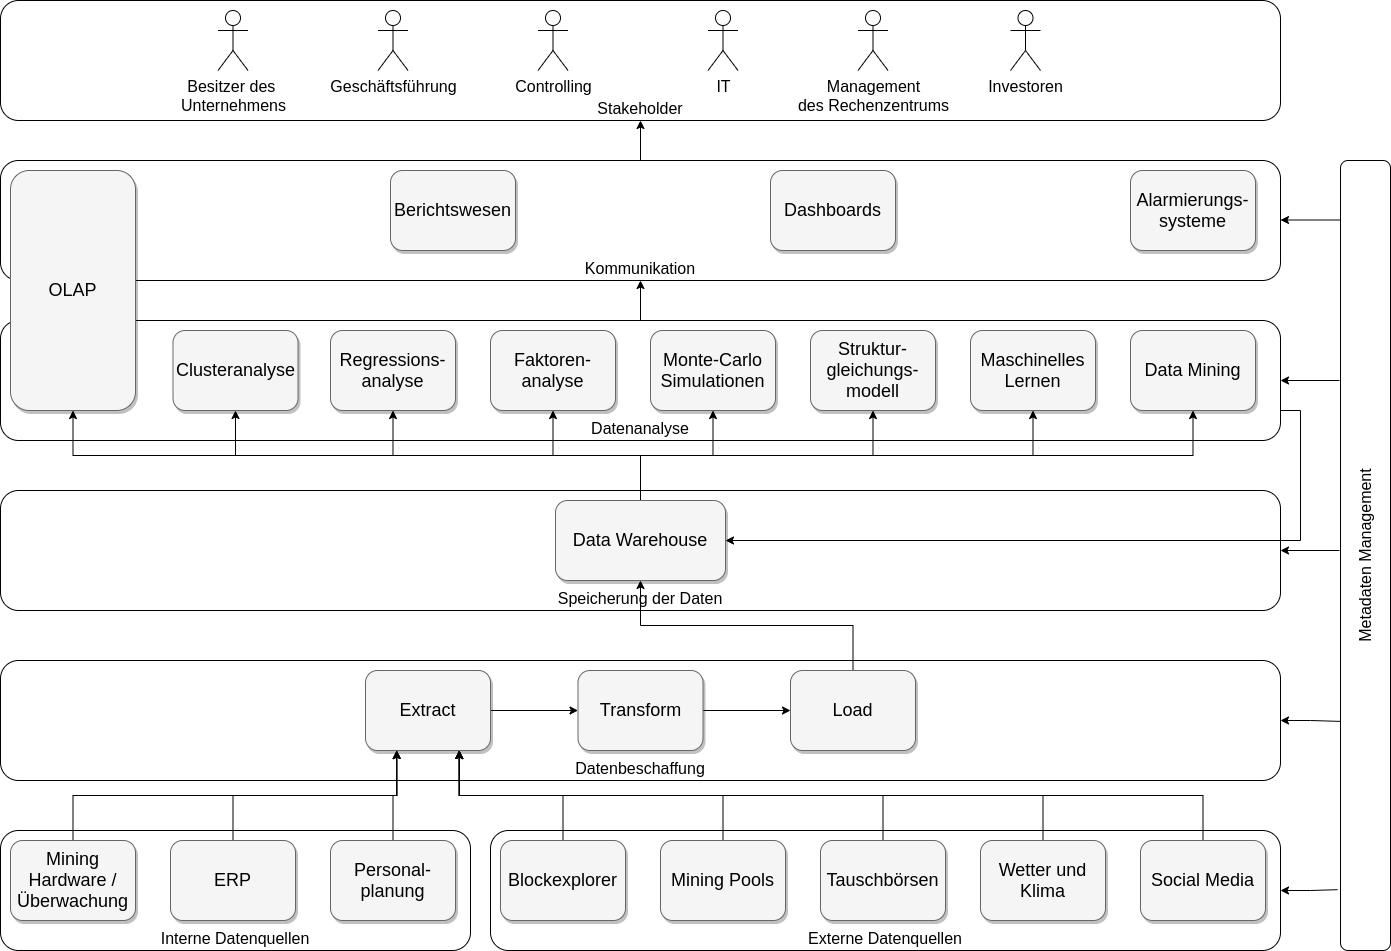
\includegraphics[width=\textwidth]{internalbiprocess}
    \label{figure:internalbiprocess}
\end{figure}

This figure is basically based on the process structure shown in chapter \ref{toc:prozess}, and is divided into the following
steps:
\begin{itemize}
    \item \textbf{Data sources: }The data sources are the services described in chapters \ref{toc:internedatenquellen} and \ref{toc:externedatenquellen}.
    All of these sources together are sufficient to provide enough data to prove the four sub-hypotheses and
    thereby the main hypothesis.
    \item \textbf{Data acquisition: }Data sourcing involves \ac{ETL} pipelines that interrogate data at the interfaces
    to the sources, transform them into the desired format, and ultimately store them in a data warehouse. As
    in the classification of data sources from table \ref{tbl:klassifizierunginternedaten} and \ref{tbl:klassifizierungexternedaten},
    as well as chapter \ref{toc:datenhaltung}, the \ac{ETL} pipelines can be built and realized without any obstacles.
    \item \textbf{Storage of data / data management: }In the third step, the extracted and structured data are loaded into a data warehouse.
    This contains all data that is still important for the \ac{BI} process to be able to present results to the stakeholders.
    This part can be implemented as shown in chapter \ref{toc:datenhaltung}.
    \item \textbf{Data analysis: }The stored data is subsequently used for analysis in order to be able to generate new knowledge.
    There are many different approaches for the analysis of data, which have been discussed in detail in chapter \ref{toc:analyseverfahrenbi}.
    These are used to find out the optimization potential of a cryptomining data center and to identify
    possible approaches for implementation. All of these forms of analysis can be implemented in-house
    without further ado. However, the exact design of the analysis algorithms is a lengthy and complex process
    and will not be discussed in the course of this thesis, since the basic possibility of implementation is discussed in this work.
    \item \textbf{Communication / Presentation: }The final step is to present the data in a manner, 
    through which the stakeholders of the \ac{BI} process can access and further use the knowledge.
    Relevant forms of presentation are described in
    chapter \ref{toc:datenpraesentation} and are sufficient to ensure that stakeholders can be guided in an optimal way through the
    \ac{BI} Process. Implementation of this level is straightforward.
\end{itemize}

In the following chapter, the conclusion from this and the last chapter is subjected to a critical evaluation in order to
finally be able to put the answer to the main hypothesis into the right context.
\newpage
\section{Summary and outlook} \label{toc:zusammenfassungundausblick}

\subsection{Hypothesis testing} \label{toc:ueberpruefungderhypothesen}

In the present thesis it was answered whether it is possible by means of application of a \ac{BI} process to optimize
mining data centers. To be able to answer this question, the first step in chapter
\ref{toc:grundlagenbusinessintelligence} and \ref{toc:grundlagenkryptomining} was the basics for understanding
business intelligence, mining of cryptocurrencies and the financial \acp{KPI} of mining data centers were laid.
This knowledge is used as the basis for the subsequent part (chapter \ref{toc:ansatzmoeglichkeitenfuerbusinessintelligence})
used to conduct a deductive reasoning that gives a first answer to the main hypothesis.
This reasoning is divided into several steps. In the first step, the available data sources were identified,
These were analyzed for suitability towards a \ac{BI} Process. Subsequently
all relevant \acp{KPI} were identified for each sub-hypothesis. The result of this analysis was that
the data sources are suitable and sufficient for the realization of a \ac{BI} Process. In the next step
various analysis procedures were listed that could be considered for processing the data.
For this purpose, these procedures were briefly described and possible examples and approaches within the sub-hypotheses were
identified. As a result, it can be determined that the analysis methods for the case of descriptive
\ac{BI} are sufficient. For predictive models, an answer is not possible at this stage. In the following chapter
(chapter \ref{toc:planungeinesbiprozessesfuereinminingrechenzentrum}) a case study was carried out on the basis of the so far elaborated
results, which took place within the Genesis Group. This case study
examines the internal feasibility of the previous results and complements them. In the first step
a stakeholder analysis was carried out. This is used for the planning of an in-house \ac{BI} Process.
Subsequently, the individual steps of the process were analyzed and possible software products identified.
In addition, a focus was placed on the presentation of the data, as this has not yet been discussed in the previous argumentation.
Finally, the case study was analyzed and a result for the main hypothesis was formed.

On the basis of the argumentation and the case study, it can be determined that the partial hypotheses and thus also the main hypothesis are
true. It is possible that data centers that mine cryptocurrencies can be financially optimized by applying a \ac{BI}
Process.

However, limitations exist with the chosen approach within this thesis. These include the following points:
\begin{itemize}
    \item Ultimately, the \ac{BI} Process in the present work has been planned in a theoretical context. Whether such a
    process actually works in reality can only be clarified by putting this planning into practice.
    However, the probability that this will not work is very low, since the case study
    should cover the practical implementation as best as possible.
    \item The various forms of analysis have been pointed out throughout the paper. However, it was decided not to
    concrete elaboration of these forms of analysis and their implementation. Therefore, only an implementation of the
    analysis algorithms can say whether these meet the requirements.
    \item The integration of a \ac{BI} Process was discussed only on the basis of the available data sources. In the absence
    or existence of additional data sources, the design of the \ac{BI} process may change in a way that is not
    been discussed in this paper. However, the data sources that have been pointed out are with a
    high probability available in any company that participates in mining. Even when using other
    types of mining hardware, the parameters may change leading to a change in the \ac{BI} process.
    \item Consensus algorithms other than \ac{PoW} were not discussed in this paper. These have to be individually adapted
    into a \ac{BI} process.
\end{itemize}

Despite these points, it is possible to consider the main hypothesis as answered, since all data sources used in this work are available in any company on the market.
Only in special cases small adjustments have to be made, but these will not change the overall conclusion of this work.

\subsection{Further research approaches} \label{toc:ausblick}

From the limitations identified in chapter \ref{toc:ueberpruefungderhypothesen}, further
research approaches can be derived. This thesis focused on \ac{BI} in the environment of the Bitcoin Blockchain and its
relevant technologies. However, other use cases of blockchain technology also exist, and their investigation in the
\ac{BI} context can be interesting. These include the following technologies, among others:

\begin{itemize}
    \item \textbf{\ac{DeFi}: }In the course of this work, cryptocurrency exchanges were used as a data source. These are by nature
    inherently centralized services provided by individual companies, such as Binance\footnote{https://www.binance.com/en}
    or Kraken\footnote{https://www.kraken.com}. Developers are already working on the decentralized equivalent of these
    services, referred to as \ac{DeFi}.\footcite[Cf.][]{wiesflecker2021trends} Also, there will be
    this technology introduces a credit system in the cryptocurrency space, which may be of particular interest to companies
    that need liquidity in cryptocurrencies.\footcite[Cf.][]{wiesflecker2021trends} The
    Exploration of the role of \ac{DeFi} in \ac{BI} is therefore a current example of a research gap building on this work.
    \item \textbf{Smart Contracts: }For some time now, so-called smart contracts have also been mapped using Blockchain
    Technology. The best-known example of this implementation is the Ethereum
    Blockchain.\footcite[Cf.][]{wiesflecker2021trends} Smart Contracts are decentralized equivalents of classical contracts
    within a blockchain.\footcite[Cf.][]{wiesflecker2021trends} As especially contracts with customers, service providers
    and suppliers are interesting for \ac{BI} systems, therefore, exploring the decentralized counterpart would be a
    gap in which research can still be done.
    \item \textbf{\acp{NFT}: }These tokens represent unique values.\footcite[Cf.][]{wiesflecker2021trends} 
    In this regard, such tokens may represent, for example, relevant investments by companies in art, instruments
    and other unique investment assets. How and whether these interact with the field of \ac{BI} can be the subject of
    of a further work on this topic. 
    \item \textbf{Other consensus algorithms and currencies: }As described at the beginning of this work, only the Bitcoin
    Blockchain and the \ac{PoW} consensus algorithm were analyzed within this thesis. Since there are other consensus algorithms,
    such as \ac{PoS}, the investigation of further cryptocurrencies and consensus algorithms would be of
    interest. Through such an investigation, this work can be suitably complemented and
    the topic of \ac{BI} and cryptocurrencies to be explored in more depth.
\end{itemize}

Based on the veracity of the main hypothesis of this work, these aspects can deepen the possible uses of \ac{BI} in the
cryptomining context in more depth and identify further potential use cases.



%-----------------------------------
% Anhang
%-----------------------------------
\newpage
\section*{Appendix} %Überschrift "Anhang", ohne Nummerierung
\addcontentsline{toc}{section}{\langde{Anhang}\langen{Appendix}} %Den Anhang ohne Nummer zum Inhaltsverzeichnis hinzufügen
\begin{appendices}
% Nachfolgende Änderungen erfolgten aufgrund von Issue 163
\makeatletter
\renewcommand\@seccntformat[1]{\csname the#1\endcsname:\quad}
\makeatother
\addtocontents{toc}{\protect\setcounter{tocdepth}{0}} %
	\renewcommand{\thesection}{\langde{Anhang}\langen{Appendix} \arabic{section}}
	\renewcommand\thesubsection{\langde{Anhang}\langen{Appendix} \arabic{section}.\arabic{subsection}}
	\section{Internal documents} \label{toc:internedokumente}

\subsection{Layout Mining Data Center} \label{toc:layoutkardok}
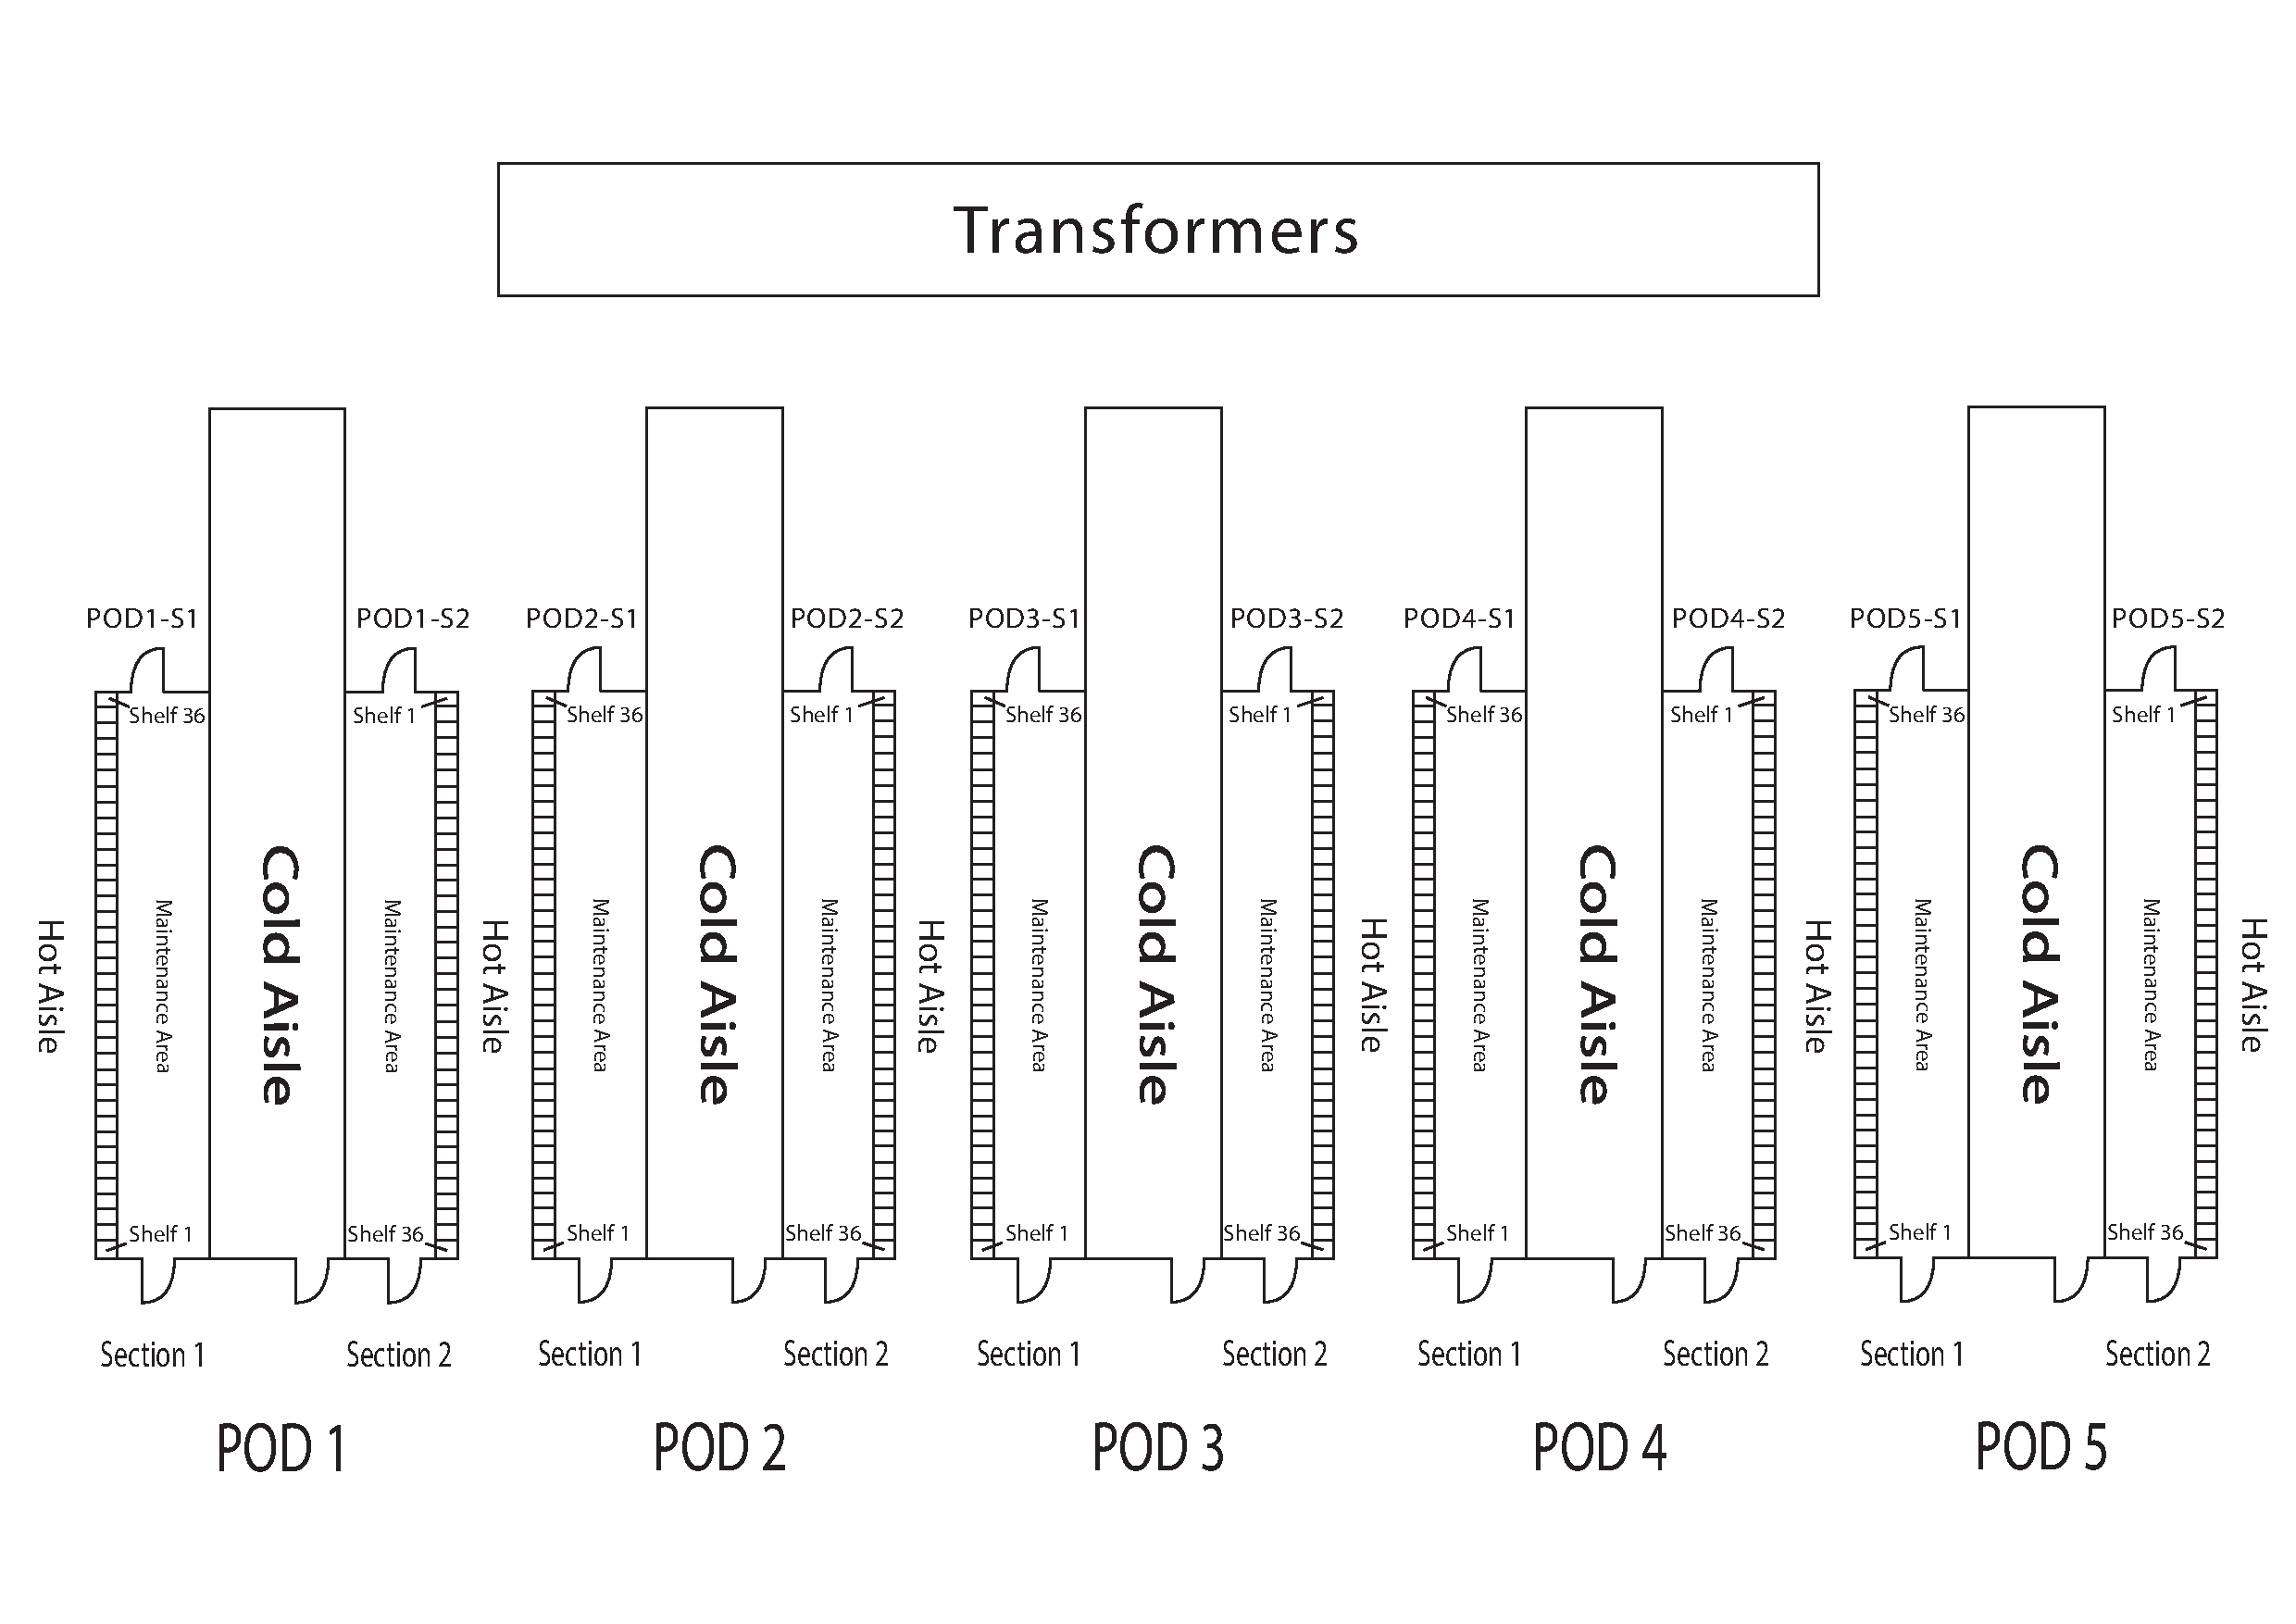
\includegraphics[page=1, angle=90, width=\linewidth]{layoutkardok.pdf} 

\newpage
\subsection{Functionality Mining Proxy} \label{toc:funktionsweiseminingproxy}
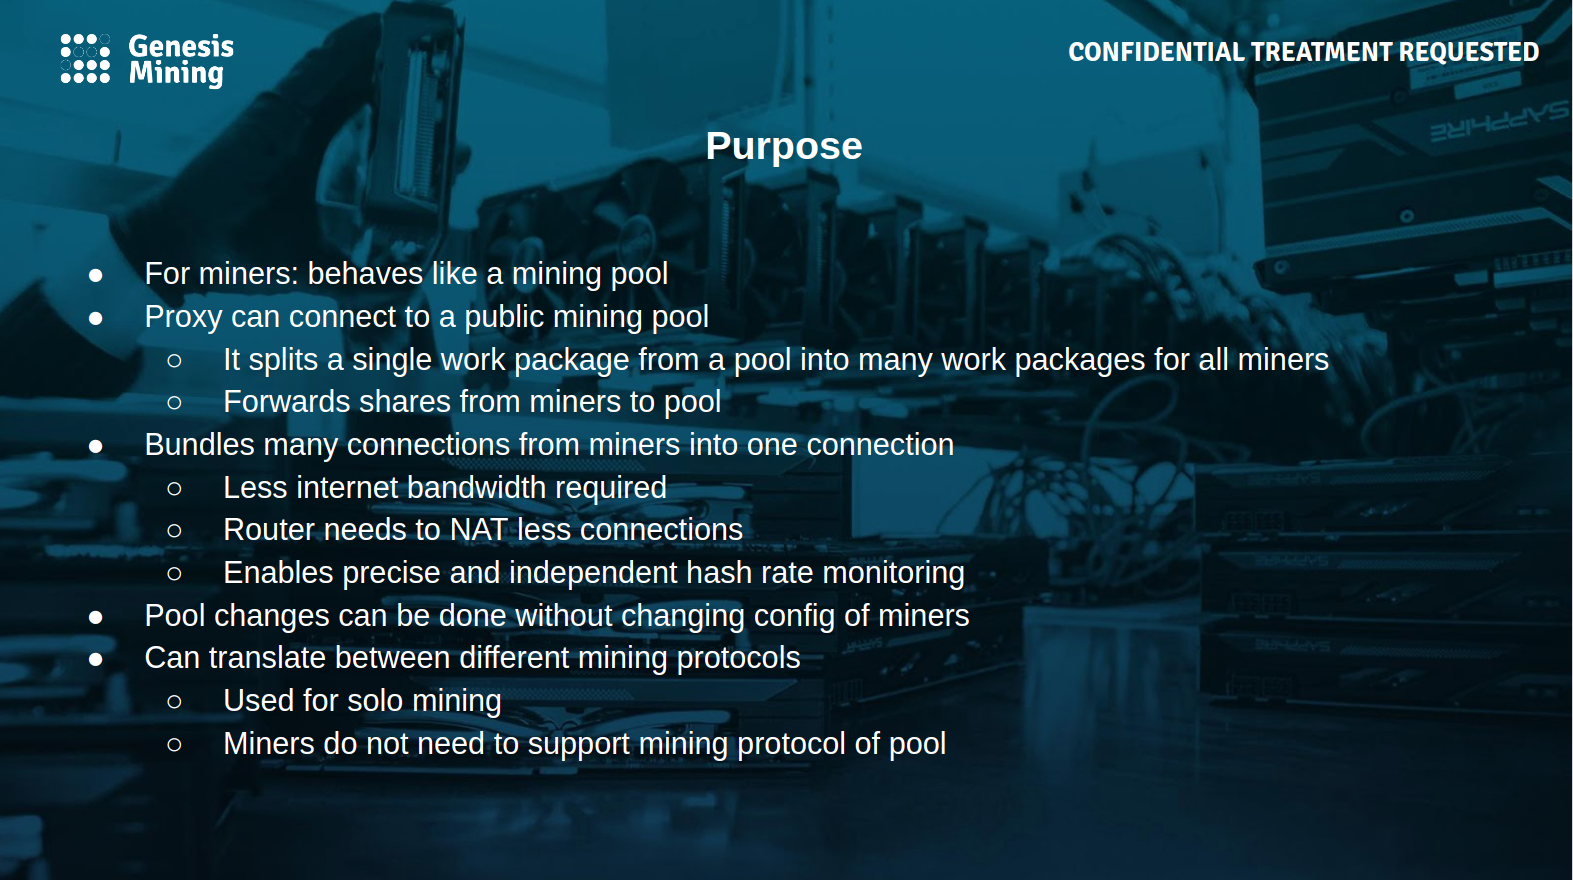
\includegraphics[width=\linewidth]{miningproxy}

\subsection{Network topology section} \label{toc:netzwerktopologieausschnitt}
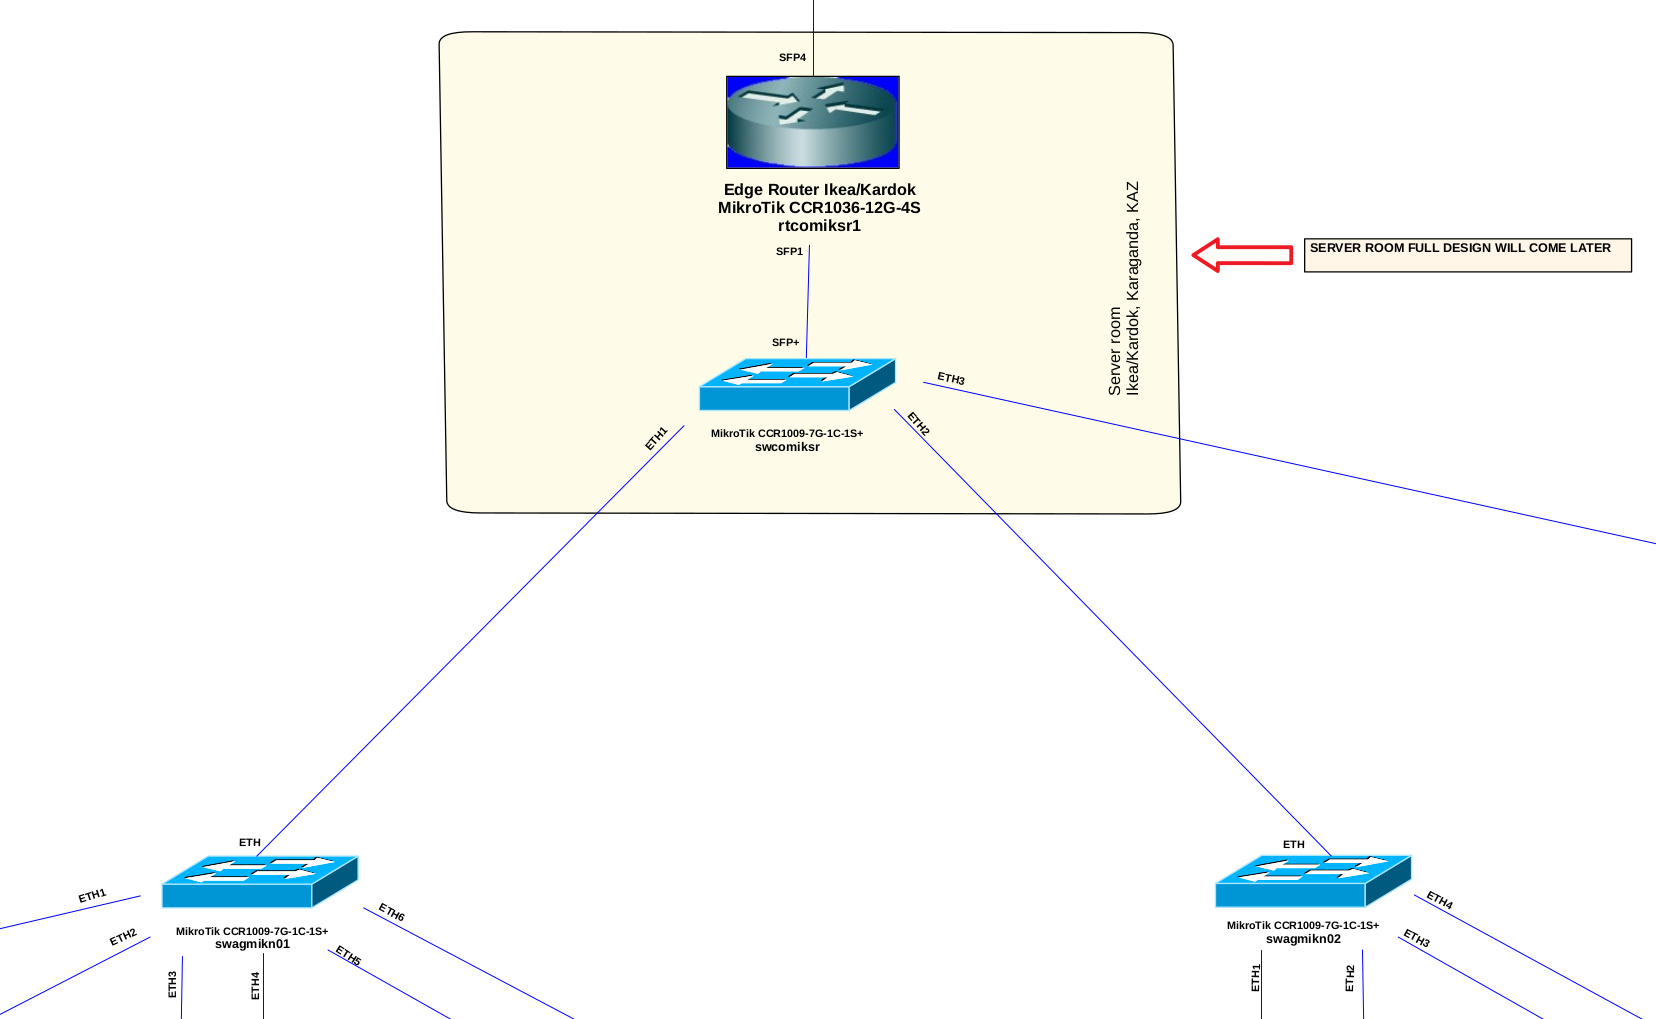
\includegraphics[width=\linewidth]{networktopologykaz}

\newpage
\subsection{Summary of Investment} \label{toc:summaryofinvestment}
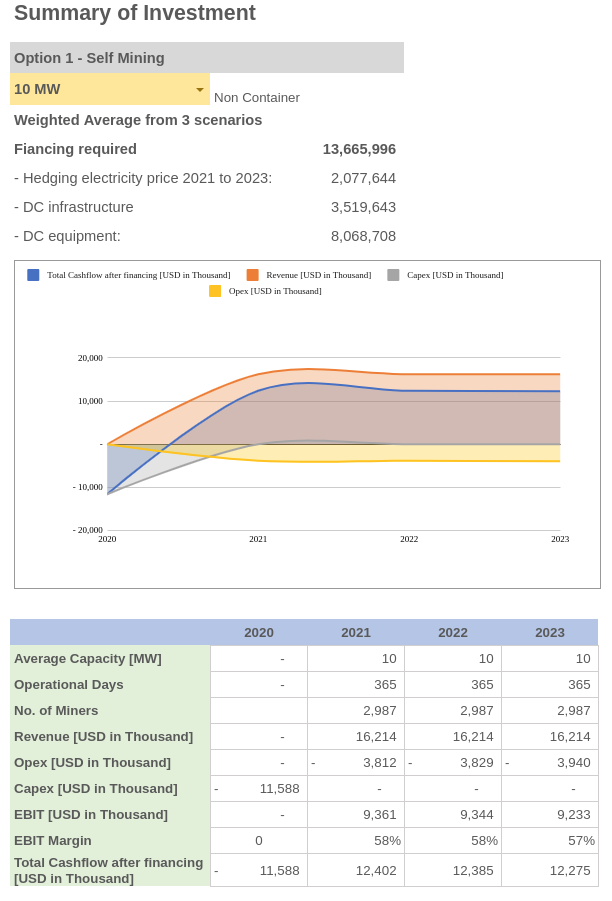
\includegraphics[width=0.7\linewidth]{summaryofinvestment}

\newpage
\subsection{CapEx} \label{toc:capex}
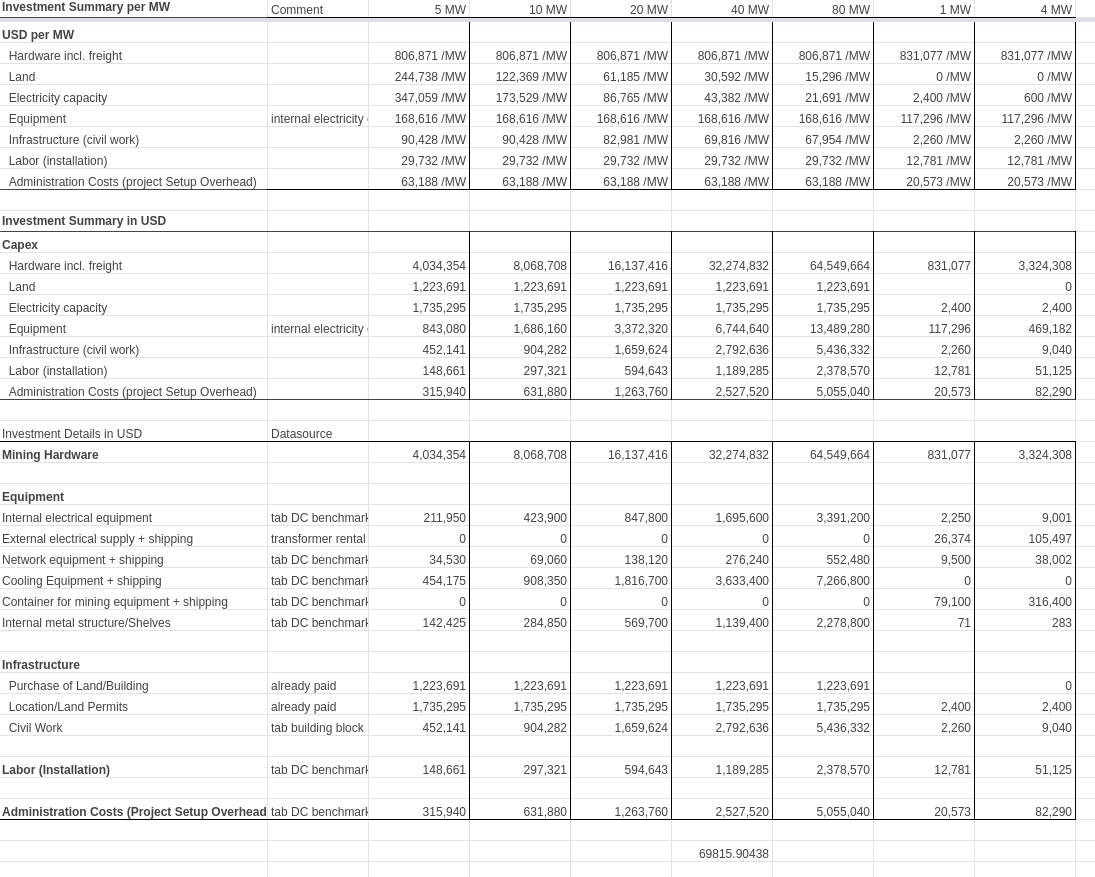
\includegraphics[width=\linewidth]{capex}

\newpage
\subsection{OpEx} \label{toc:opex}
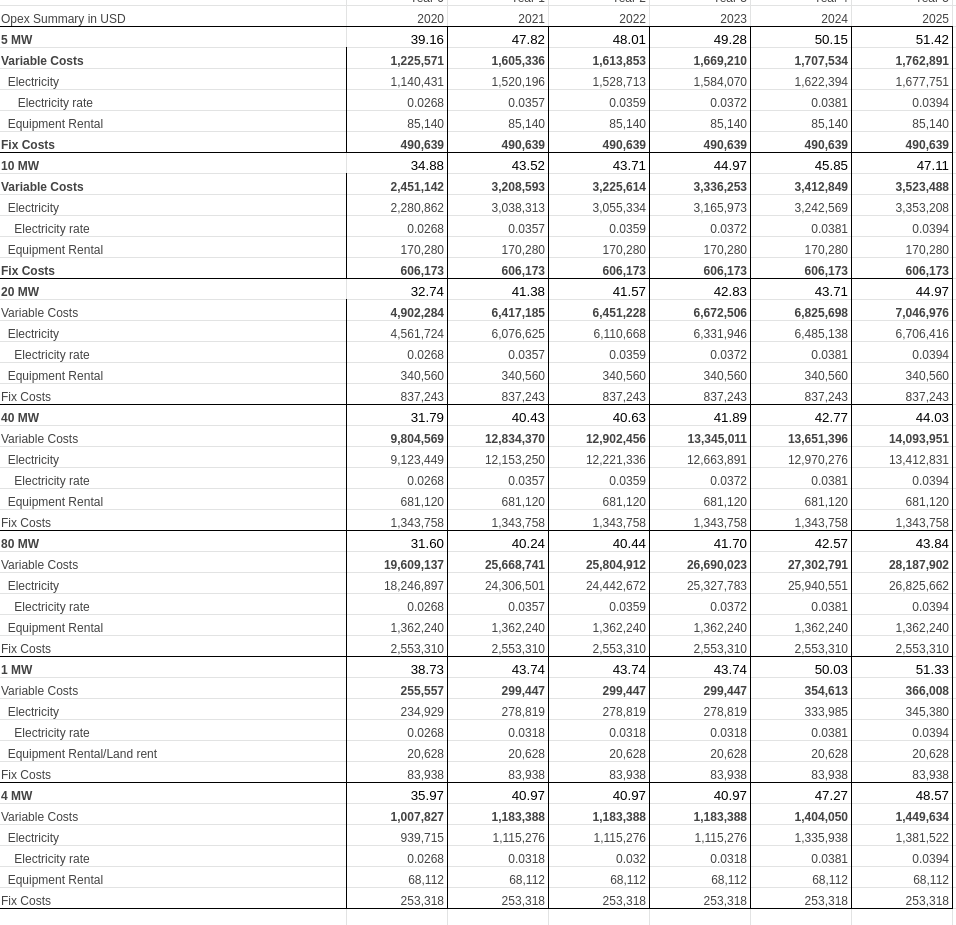
\includegraphics[width=\linewidth]{opex}

\newpage
\subsection{S19Pro Assumptions} \label{toc:s19proassumptions}
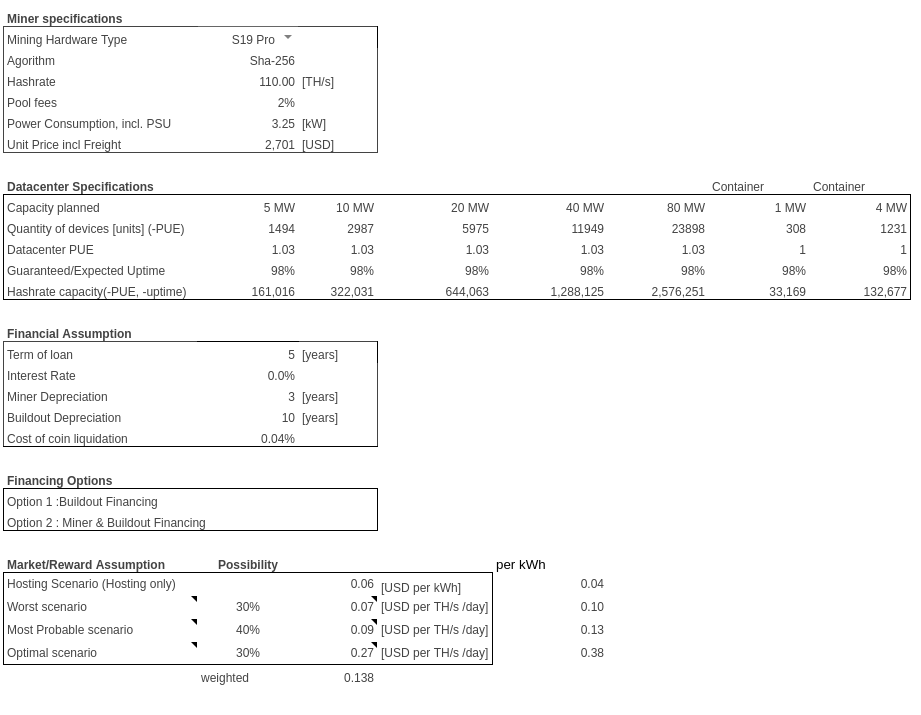
\includegraphics[width=\linewidth]{minerassumptions}

\newpage
\subsection{Funding Worst-case scenario} \label{toc:finanzierungworstcase}
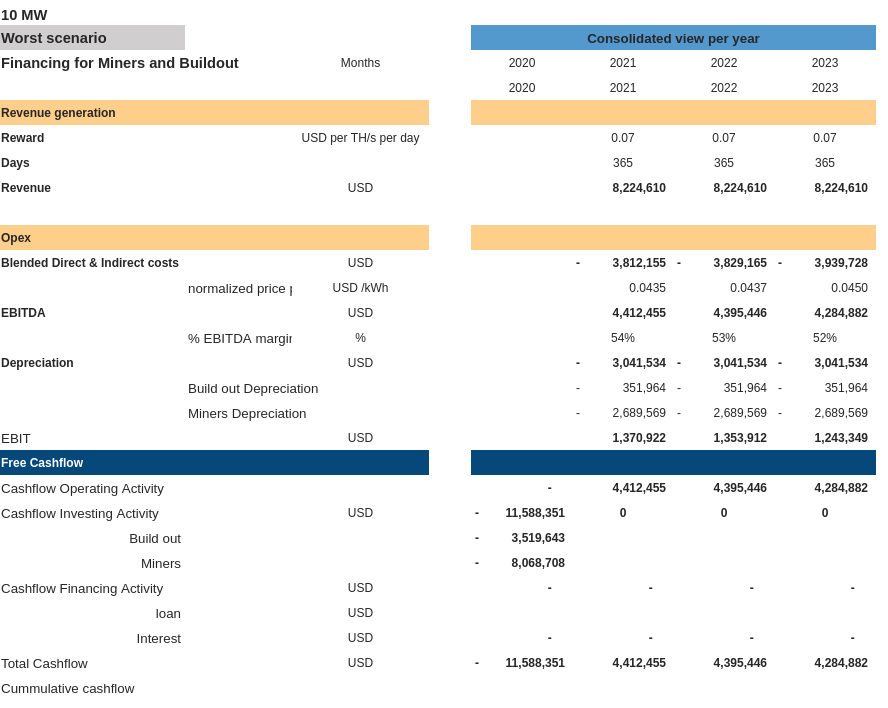
\includegraphics[width=\linewidth]{financingworstscenario}

\newpage
\subsection{Funding Most-Probable Scenario} \label{toc:finanzierungmostprobable}
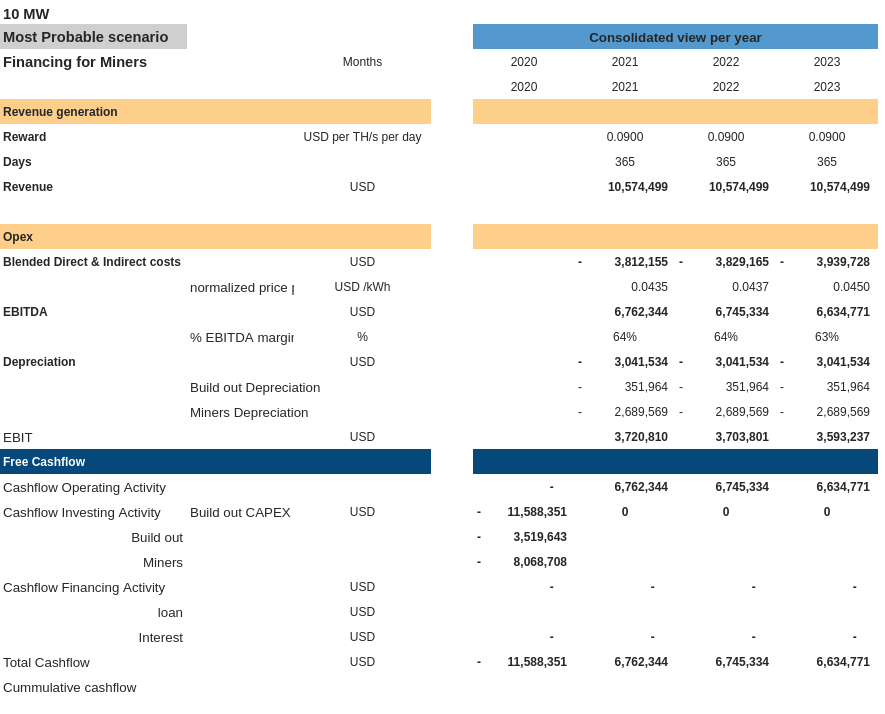
\includegraphics[width=\linewidth]{financingprobablescenario}

\newpage
\subsection{Funding optimal scenario} \label{toc:finanzierungoptimal}
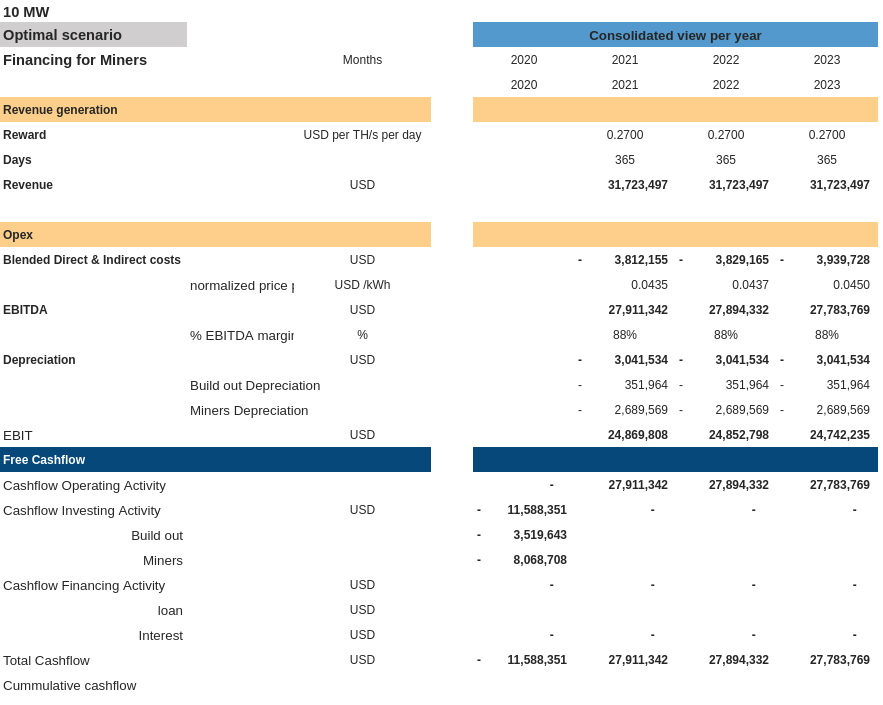
\includegraphics[width=\linewidth]{financingoptimalscenario}

\newpage
\subsection{Different runs of a Bitcoin price and hashrate Monte Carlo simulation. (06.11.2020)} \label{toc:montecarlosimulationvier}
\includegraphics[page=2, width=\linewidth]{monte-carlo.pdf}

\newpage
\subsection{Evolution of the Bitcoin price based on a Monte Carlo simulation (06.11.2020)} \label{toc:entwicklungbitcoinpreismc}
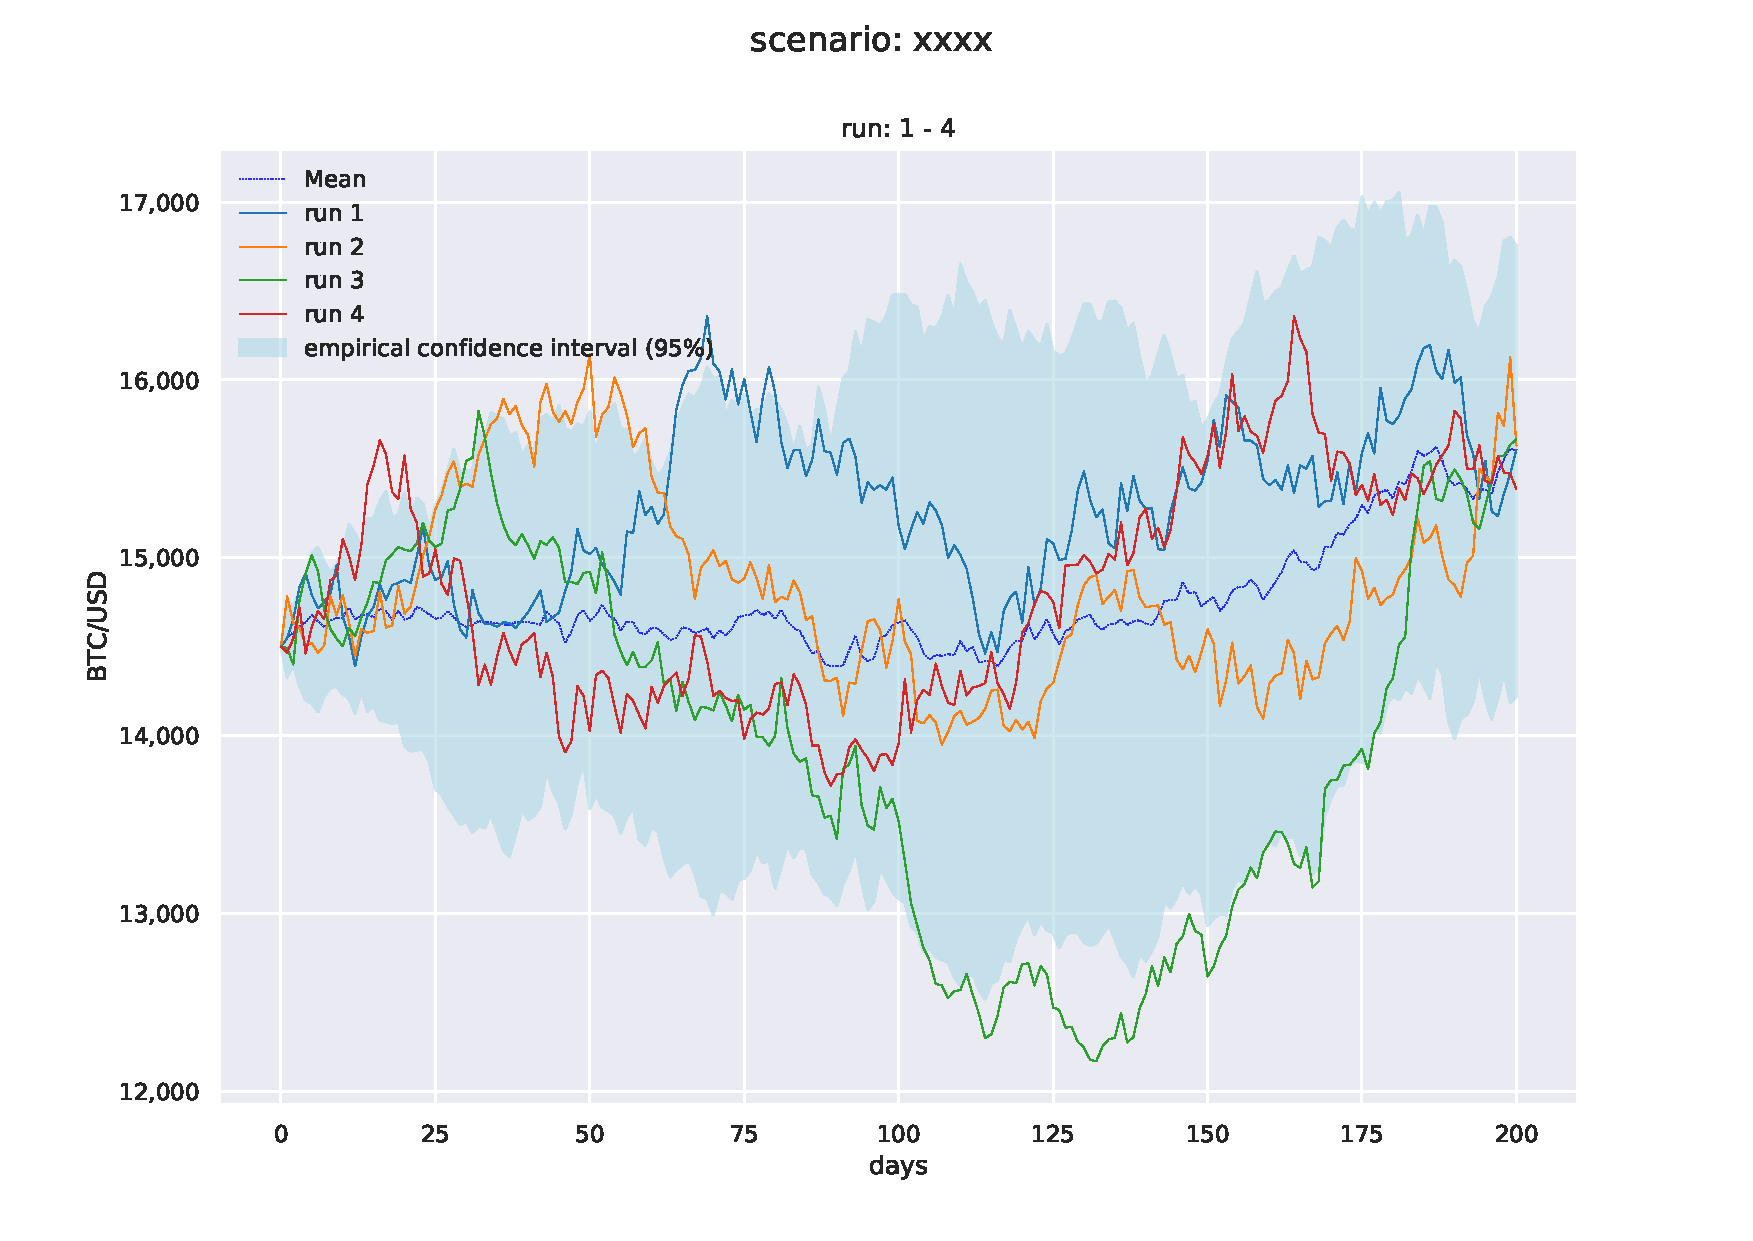
\includegraphics[page=1, width=\linewidth]{monte-carlo.pdf}

\newpage
\subsection{Evolution of Bitcoin's network hashrate based on Monte Carlo simulation. (06.11.2020)} \label{toc:entwicklunghashratemc}
\includegraphics[page=6, width=\linewidth]{monte-carlo.pdf}

\newpage
\subsection{Evolution of \ac{BTC} and \ac{USD} exchange rate starting from 06.11.2020}
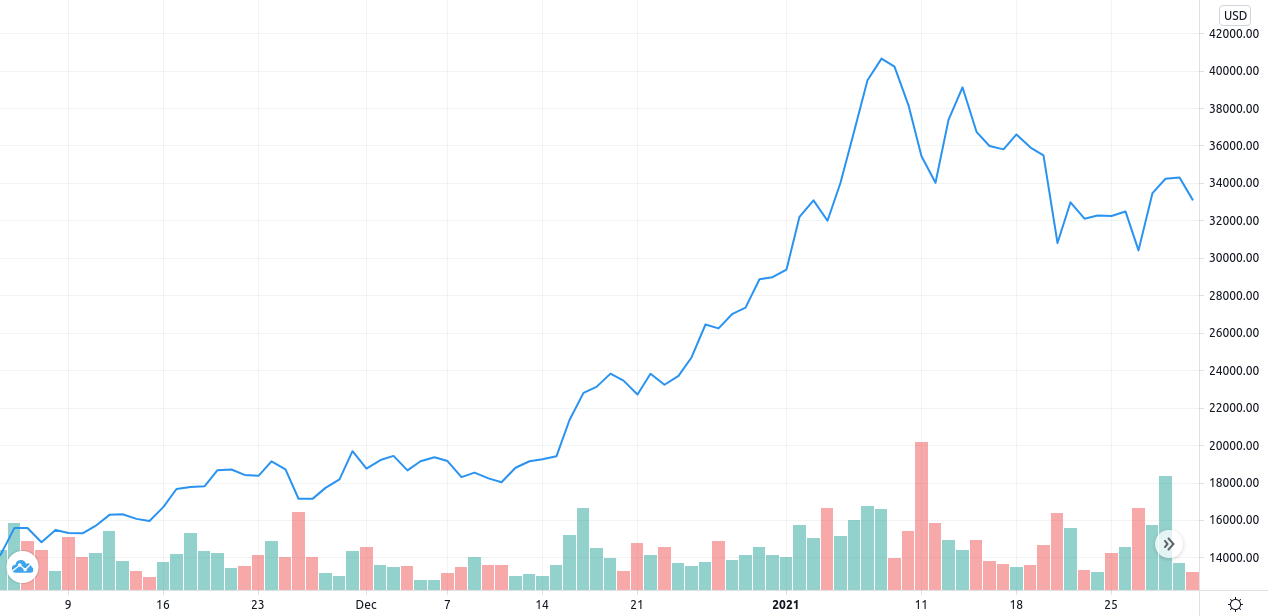
\includegraphics[width=\linewidth]{btcusd}
\cite[Source:][]{tradingview2021btcusd}

\newpage
\section{Literature research} \label{toc:literaturrecherche}
\subsection{Literature taxonomy} \label{toc:literaturtaxonomie}

\begin{table}[H]
    \caption{Literature taxonomy}
    \label{tbl:literaturtaxonomie}
    \scriptsize
    \begin{tabularx}{\textwidth}[ht]{|X||X|X|X|X|}
		\hline
		\textbf{Charasteristic} & \multicolumn{4}{X|}{\textbf{Categories}} \\
		\hline\hline
			Focus & Research Outcomes & Research Methods & \checkmark \textbf{Theories} & \checkmark \textbf{Applications} \\
		\hline
			Goal & \checkmark \textbf{Integration} & Criticism & \checkmark \textbf{Central Issues} & \\
		\hline
			Organisation & Historical & \checkmark \textbf{Conceptual} & Methodological & \\
		\hline
			Perspective & \checkmark \textbf{Neutral Representiation} & Espousal of Position & & \\
		\hline  
			Audience & \checkmark \textbf{Specialised Scholars} & General Scholars & Practitioners and Politicians & General Public \\
		\hline
			Coverage & Exhaustive & Exhaustive and Selective & Representative & \checkmark \textbf{Central/Pivotal} \\
		\hline
    \end{tabularx}
    \cite[Source: Based on][]{cooper1988organizing}
\end{table}
  
\subsection{Results of the search process} \label{toc:suchprozessergebnis}

\begin{table}[H]
	\caption{Literature research}
	\label{tbl:suchprozessergebnis}
  	% \tiny
	\scriptsize
  	\begin{tabularx}{\textwidth}[ht]{|l|X|X|l|l|X|l|X|X|}
		\hline
		\textbf{No.} & \textbf{Title} & \textbf{Author} & \textbf{Year} & \textbf{Date} & \textbf{Search term} & \textbf{Search engine} & \textbf{Relevance} \\
		\hline\hline
		1 & How Elon Musk’s Twitter Activity Moves Cryptocurrency Markets & Ante & 2021 & 20.03.2021 & Bitcoin AND Tweet AND Elon AND Musk & Google Scholar & Influence of Social Media on the Bitcoin Price \\
		\hline
		2 & Business intelligence as a key strategy for development organizations & Azma \& Mostafapour & 2012 & 18.12.2020 & Loshin AND Business AND Intelligence & Google Scholar & Introduction BI \\
		\hline
		3 & Bitcoin as a transaction ledger: A composable treatment & Badertscher et al. & 2017 & 07.02.2021 & Bitcoin AND Ledger & Google Scholar & Poor predictability of BTC rates \\
		\hline
		4 & Bitcoin mining technology & Bhaskar \& Chuen & 2015 & 07.02.2021 & Bitcoin AND Cloud AND Mining & Google Scholar & Mining Pools, Cloud Mining, Hardware, Blockchain \\
		\hline
		5 & A comparative study of data analysis techniques & Bihani \& Patil & 2014 & 23.03.2021 & Business AND Analytics & Google Scholar & Types of Business Analytics \\
		\hline
		6 & Bitcoin Intelligence–Business Intelligence meets Crypto Currency & Boto{\c{s}} & 2017 & 06.02.2021 & Mining AND Cryptocurrency AND Business AND Intelligence & Google Scholar & BI and Cryptocurrencies \\
		\hline
		7 & Business intelligence strategy & Boyer et al. & 2010 &  & \textit{Buch im Besitz des Autors} & & BI Basics \\
		\hline
		8 & Modeling and Simulation of the Economics of Mining in the Bitcoin Market & Cocco \& Marchesi & 2016 & 05.04.2021 & Monte AND Carlo AND Simulation AND Bitcoin & Google Scholar & Use of Monte Carlo simulations \\
		\hline
	\end{tabularx}
\end{table}

\begin{table}[H]
	\scriptsize
  	\begin{tabularx}{\textwidth}[ht]{|l|X|X|l|l|X|l|X|X|}
		\hline
		\textbf{No.} & \textbf{Title} & \textbf{Author} & \textbf{Year} & \textbf{Date} & \textbf{Search term} & \textbf{Search engine} & \textbf{Relevance} \\
		\hline\hline
		9 & Optimizing sha256 in bitcoin mining & Courtois \& Grajek & 2014 & 06.02.2021 & Mining AND Cryptocurrency AND Optimization & Google Scholar &  \\
		\hline
		10 & From chaining blocks to breaking even: A study on the profitability of bitcoin mining from 2012 to 2016 & Derks et al. & 2018 & 07.02.2021 & Bitcoin AND Mining AND Venture & Google Scholar & Value and cost flows, cash flow, mining hardware \\
		\hline
		11 & What is business intelligence? & Foley, Guillemette & 2010 & 18.12.2020 & ((Business AND Intelligence) OR BI) AND Costs & Google Scholar & History, definition BI, BI process components \\
		\hline
		12 & Disrupting industries with blockchain: The industry, venture capital funding, and regional distribution of blockchain ventures & Friedlmaier et al. & 2017 & 07.02.2021 & Bitcoin AND Mining AND Venture & Google Scholar & Share of mining companies in startups \\
		\hline
		13 & Blockchain meets cloud computing: a survey & Gai et al. & 2020 & 06.02.2021 & Crypto AND Mining AND Optimization AND Hardware & Google Scholar & Cloud Mining \\
		\hline
		14 & Fallstudien als Forschungsmethode: Pl{\"a}doyer f{\"u}r einen Methodenpluralismus in der deutschen betriebswirtschaftlichen Forschung & Göthlich & 2003 & 11.03.2021 & \textit{Vorwärtssuche basierend auf Wilde \& Hess} &  & Methodology Case studies \\
		\hline
		15 & Demystifying crypto-mining: Analysis and optimizations of memory-hard pow algorithms & Han et al. & 2019 & 06.02.2021 & Mining AND Cryptocurrency AND Optimization & IEEExplore & Consensus algorithms \\
		\hline
		16 & Capturing value from big data--a taxonomy of data-driven business models used by start-up firms & Hartmann et al. & 2016 & 18.12.2020 & Data AND Driven AND Business & EBSCO & Data model, Key data, Key activities, Value proposition \\
		\hline
		17 & Assessing benefits of business intelligence systems--a case study & Ho{\v{c}}evar \& Jakli{\v{c}} & 2010 & 18.12.2020 & ((Business AND Intelligence) OR BI) AND Costs & Google Scholar & Added value BI, advantages through BI \\
		\hline
		18 & Business intelligence and implementation in a small enterprise & Horakova \& Skalska & 2013 & 18.12.2020 & ((Business AND Intelligence) OR BI) AND Implementation & Google Scholar & Stakeholders, added value, introduction of BI \\
		\hline
		19 & Data quality & Huh et al. & 1990 & 26.03.2021 & Data AND Quality & Google Scholar & Quality criteria for data \\
		\hline
  	\end{tabularx}
\end{table}

\begin{table}[H]
	\scriptsize
  	\begin{tabularx}{\textwidth}[ht]{|l|X|X|l|l|X|l|X|X|}
		\hline
		\textbf{No.} & \textbf{Title} & \textbf{Author} & \textbf{Year} & \textbf{Date} & \textbf{Search term} & \textbf{Search engine} & \textbf{Relevance} \\
		\hline\hline
		20 & Bitcoin Network Mechanics: Forecasting the BTC Closing Price Using Vector Auto-Regression Models Based on Endogenous and Exogenous Feature Variables & Ibrahim et al. & 2020 & 30.03.2021 & Forecasting AND Bitcoin AND Price AND Regression & Google Scholar & Prediction models bitcoin price \\
		\hline
		21 & Business intelligence (BI) success and the role of BI capabilities & Isik et al. & 2011 & 18.12.2020 & ((Business AND Intelligence) OR BI) AND Risk & Google Scholar & BI in general \\
		\hline
		22 & Business intelligence: An analysis of the literature & Jourdan et al. & 2008 & 18.12.2020 & (Business AND Intelligence) OR BI & Google Scholar & Methodology and BI \\
		\hline
		23 & The fundamentals of business intelligence & Kasemsap & 2016 & 18.12.2020 & Loshin AND Business AND Intelligence & Google Scholar & ROI Hypothese, BI in general \\
		\hline
		24 & Big data and business intelligence: Debunking the myths & Kimble \& Milolidakis & 2015 & 26.03.2021 & Data AND In AND Business AND Intelligence & Google Scholar & Data types for BI \\
		\hline
		25 & Understanding Information System agility--the example of business intelligence & Knabke \& Olbrich & 2013 & 18.12.2020 & ((Business AND Intelligence) OR BI) AND Scrum & Google Scholar & Literature Review, Definition of Agility \\
		\hline
		26 & The economics of Bitcoin mining, or Bitcoin in the presence of adversaries & Kroll et al. & 2013 & 07.02.2021 & Bitcoin AND Mining & Google Scholar & Explanation of mining \\
		\hline
		27 & Blockchain-enabled data provenance in cloud datacenter reengineering & Li et al. & 2019 & 06.02.2021 & Crypto AND Mining AND Data AND Center & Google Scholar & Explanation of PoW \\
		\hline
		28 & Business intelligence: the savvy manager's guide & Loshin & 2012 &  & \textit{Buch im Besitz des Autors} &  & BI Basics \\
		\hline
		29 & Grundz{\"u}ge der Wirtschaftsinformatik & Mertens et al. & 2005 & & & & Definition Business Informatics \\
		\hline
		30 & A brief survey of cryptocurrency systems & Mukhopadhyay et al. & 2016 & 17.02.2021 & Mining AND Cryptocurrency & Google Scholar & BTC history \\
		\hline
		31 & Agile BI-The Future of BI. & Muntean \& Surcel & 2013 & 18.12.2020 & ((Business AND Intelligence) OR BI) AND Scrum & Google Scholar & BI process, Scrum as methodology \\
		\hline
		32 & Bitcoin: A peer-to-peer electronic cash system & Nakamoto & 2008 & 07.02.2021 & Bitcoin AND Whitepaper & Google Scholar & Bitcoin, Blockchain, Mining \\
		\hline
		33 & Cognition-driven decision support for business intelligence & Niu et al. & 2009 & 18.12.2020 & Business Intelligence OR BI & Google Scholar & BI process, OLAP, warehouses, analysis options \\
		\hline
		34 & Big data business intelligence in bank risk analysis & Rahman \& Iverson & 2015 & 18.12.2020 & ((Business AND Intelligence) OR BI) AND Risk & Google Scholar & IT Architecture Big Data \\
		\hline
		35 & Business justification with business intelligence & Ranjan & 2008 & 18.12.2020 & Loshin AND Business AND Intelligence & EBSCO & BI Definition and Components \\
		\hline
	\end{tabularx}
\end{table}

\begin{table}[H]
	\scriptsize
  	\begin{tabularx}{\textwidth}[ht]{|l|X|X|l|l|X|l|X|X|}
		\hline
		\textbf{No.} & \textbf{Title} & \textbf{Author} & \textbf{Year} & \textbf{Date} & \textbf{Search term} & \textbf{Search engine} & \textbf{Relevance} \\
		\hline\hline
		36 & Who's in and why? A typology of stakeholder analysis methods for natural resource management & Reed et al. & 2009 & 01.04.2021 & Stakeholder AND Analysis AND Business AND Intelligence & Google Scholar & Stakeholder analysis \\
		\hline
		37 & A stakeholder model of business intelligence & Simmers & 2004 & 11.03.2021 & Stakeholder AND Business AND Intelligence & Google Scholar & Stakeholder analysis \\
		\hline
		38 & The usefulness of ERP systems for effective management & Spathis \& Constantinides & 2003 & 22.03.2021 & ERP AND Systems AND Financial AND Accounting & Google Scholar & Overview ERP \\
		\hline
		39 & The evolution of bitcoin hardware & Taylor & 2017 & 06.02.2021 & Crypto AND Mining AND Optimization AND Hardware & IEEExplore & History of mining \\
		\hline
		40 & Key success factors to business intelligence solution implementation & Villamar\'{i}n \& Diaz Pinzon & 2017 & 18.12.2020 & Loshin AND Business AND Intelligence & Google Scholar & Role PM and Top Management in BI \\
		\hline
		41 & The current state of business intelligence & Watson \& Wixom & 2007 & 18.12.2020 & (Business AND Intelligence) OR BI & Google Scholar & BI Benefits, BI Success, History \\
		\hline
		42 & Methodenspektrum der Wirtschaftsinformatik & Wilde \& Hess & 2006 & 11.03.2021 & Methoden AND Wirtschaftsinformatik & Google Scholar & Overview methodologies \\
		\hline
		43 & Forschungsmethoden der Wirtschaftsinformatik & Wilde \& Hess & 2007 & 11.03.2021 & Methoden AND Wirtschaftsinformatik & Google Scholar & Overview methodologies \\
		\hline
		44 & The business value of business intelligence & Williams \& Williams & 2003 & 18.12.2020 & ((Business AND Intelligence) OR BI) AND Project AND Management & Google Scholar & Added value BI \\
		\hline
		45 & Extreme datacenter specialization for planet-scale computing: Asic clouds & Xie et al. & 2018 & 06.02.2021 & Crypto AND Mining AND Data AND Center & Google Scholar & ASIC Clouds \\
		\hline
		46 & Critical success factors for business intelligence systems & Yeoh \& Koronius & 2010 & 18.12.2020 & (Business Intelligence OR BI) AND Project AND Management & Google Scholar & Definition BI \\
		\hline
		47 & Managing the implementation of business intelligence systems: a critical success factors framework & Yeoh et al. & 2008 & 18.12.2020 & (Business Intelligence OR BI) AND Project AND Management & Google Scholar & Requirements BI and IS \\
		\hline
	\end{tabularx}
\end{table}

\newpage
Internet sources:

\begin{table}[H]
	\scriptsize
  	\begin{tabularx}{\textwidth}[ht]{|l|X|X|l|l|X|l|X|X|}
		\hline
		\textbf{No.} & \textbf{Title} & \textbf{Author} & \textbf{Year} & \textbf{Date} & \textbf{Search term} & \textbf{Search engine} & \textbf{Relevance} \\
		\hline\hline
		48 & Configure privileged API access for Antminer & Awesome Miner & & 22.03.2021 & & & Mining Hardware API \\
		\hline
		49 & Bitcoin Price in USD vs. Tweets historical chart & bitinfocharts.com & 20.03.2021 & 20.03.2021 & & & Influence of Social Media on the Bitcoin Price \\
		\hline
		50 & S19 Pro Server Installation Guide & Bitmain & 01.04.2020 & 22.03.2021 & & & Mining hardware functionality \\
		\hline
		51 & Bitcoin Developer APIs & blockchain.com & 20.03.2021 & 20.03.2021 & & & Blockchain interface \\
		\hline
		52 & Total Hash Rate (TH/s) & blockchain.com & 20.03.2021 & 20.03.2021 & & & Hashrate von Bitcoin \\
		\hline
		53 & Pool Distribution (calulate by blocks) & btc.com & 07.02.2021 & 07.02.2021 & Große AND Bitcoin AND Miner & Google & Hashrate distribution \\
		\hline
		54 & getdifficulty & developer.bitcoin.org & 20.03.2021 & 20.03.2021 & & & Blockchain interface \\
		\hline
		55 & getrawmempool & developer.bitcoin.org & 20.03.2021 & 20.03.2021 & & & Blockchain interface \\
		\hline
		56 & What is a data warehouse? & Google Cloud & & 12.04.2021 & Google AND Cloud AND Data AND Warehouse & Google & Google Cloud products \\
		\hline
		57 & Google Cloud Scheduler & Google Cloud Scheduler & & 14.04.2021 & Google AND Cloud AND Cronjobs & Google & Google Cloud products \\
		\hline
		58 & S19 Pro Specifications & Jocelyn & 27.02.2020 & 23.02.2021 & S19 Pro AND Miner AND Spec & Google & Power consumption S19 Pro Miner \\
		\hline
		59 & Bitcoin-Halving abgeschlossen: Ab jetzt nur noch 6,25 BTC pro Block & Klee & 11.05.2020 & 19.02.2021 & Bitcoin AND Halving & Google & Current Block Reward \\
		\hline
		60 & Der unersättliche Stromfresser: Bitcoin & Rooks & 16.02.2021 & 19.02.2021 & Mining AND Stromverbrauch & Google & Power consumption Mining \\
		\hline
		61 & How Elon Musk Moves The Price Of Bitcoin With His Twitter Activity & Shelvin & 21.02.2021 & 20.03.2021 & Bitcoin AND Tweet AND Elon AND Musk & Google & Influence of Social Media on the Bitcoin Price \\
		\hline
		62 & BTCUSD & tradingview.com & 29.04.2021 & 29.04.2021 & Bitcoin AND Price AND Charts & Google & Bitcoin price evolution \\
		\hline
		63 & The top 10 blockchain trends for 2021 & Wiesflecker & 26.02.2021 & 21.04.2021 & Blockchain AND Technology AND Trends & Google & Trends in blockchain technology \\
		\hline
		64 & Pricing & World Weather Online & 20.03.2021 & 20.03.2021 & & & Weather data interface \\
		\hline
		65 & Weather API & World Weather Online & 20.03.2021 & 20.03.2021 & & & Weather data interface \\
		\hline
	\end{tabularx}
\end{table}

\subsection{Concept matrix} \label{toc:konzeptmatrix}

\begin{table}[H]
    \caption{Concept matrix}
	\label{tbl:konzeptmatrix}
	\scriptsize
    \begin{tabularx}{\textwidth}[ht]{|l|X|X|X|X|X|X|X|X|}
		\hline
		\textbf{Source no. according to table \ref{tbl:suchprozessergebnis}} & \multicolumn{6}{c|}{\textbf{Concepts}} \\
		& {Business Intelligence} & {Blockchain \& Mining} & {Stakeholder analysis} & {(Big) Data} & {Cloud} & {Methodology} \\
		\hline\hline
		1 &  & \centering \checkmark &  & \centering \checkmark &  & \tabularnewline \hline
		2 & \centering \checkmark &  &  &  &  & \tabularnewline \hline
		3 &  & \centering \checkmark &  &  &  & \tabularnewline \hline
		4 &  & \centering \checkmark &  &  &  & \tabularnewline \hline
		5 &  &  &  & \centering \checkmark &  & \tabularnewline \hline
		6 & \centering \checkmark & \centering \checkmark &  &  &  & \tabularnewline \hline
		7 & \centering \checkmark &  &  &  &  & \tabularnewline \hline
		8 &  & \centering \checkmark &  & \centering \checkmark &  & \tabularnewline \hline
		9 &  & \centering \checkmark &  &  &  & \tabularnewline \hline
		10 &  & \centering \checkmark &  & \centering \checkmark &  & \tabularnewline \hline
		11 &  & \centering \checkmark &  &  &  & \tabularnewline \hline
		12 &  & \centering \checkmark &  &  &  & \tabularnewline \hline
		13 &  & \centering \checkmark &  &  & \centering \checkmark & \tabularnewline \hline
		14 &  &  &  &  &  & \centering \checkmark \tabularnewline \hline
		15 & \centering \checkmark &  &  &  &  & \tabularnewline \hline
		16 &  &  &  & \centering \checkmark &  & \centering \checkmark \tabularnewline \hline
		17 & \centering \checkmark &  &  &  &  & \tabularnewline \hline
		18 & \centering \checkmark &  &  &  &  & \tabularnewline \hline
		19 &  &  &  & \centering \checkmark &  & \tabularnewline \hline
		20 &  & \centering \checkmark &  & \centering \checkmark &  & \tabularnewline \hline
		21 & \centering \checkmark &  &  &  &  & \tabularnewline \hline
		22 & \centering \checkmark &  &  &  &  & \centering \checkmark \tabularnewline \hline
		23 & \centering \checkmark &  &  &  &  & \tabularnewline \hline
		24 & \centering \checkmark &  &  & \centering \checkmark &  & \tabularnewline \hline
		25 & \centering \checkmark &  &  &  &  & \tabularnewline \hline
		26 &  & \centering \checkmark &  & \centering \checkmark &  & \tabularnewline \hline
		27 &  & \centering \checkmark &  &  & \centering \checkmark & \tabularnewline \hline
		28 & \centering \checkmark &  &  &  &  & \tabularnewline \hline
		29 &  &  &  &  &  & \centering \checkmark \tabularnewline \hline
		30 &  & \centering \checkmark &  &  &  & \tabularnewline \hline
		31 & \centering \checkmark &  &  &  &  & \tabularnewline \hline
		32 &  & \centering \checkmark &  &  &  & \tabularnewline \hline
		33 & \centering \checkmark &  &  &  &  & \tabularnewline \hline
		34 & \centering \checkmark &  &  & \centering \checkmark &  & \tabularnewline \hline
		35 & \centering \checkmark &  &  &  &  & \tabularnewline \hline
		36 & \centering \checkmark &  & \centering \checkmark &  &  & \tabularnewline \hline
		37 & \centering \checkmark &  & \centering \checkmark &  &  & \tabularnewline \hline
		38 & \centering \checkmark &  &  &  &  & \tabularnewline \hline
		39 &  & \centering \checkmark &  &  &  & \tabularnewline \hline
		40 & \centering \checkmark &  &  &  &  & \tabularnewline \hline
		41 & \centering \checkmark &  &  &  &  & \tabularnewline \hline
		42 &  &  &  &  &  & \centering \checkmark \tabularnewline \hline
		43 &  &  &  &  &  & \centering \checkmark \tabularnewline \hline
		44 & \centering \checkmark &  &  &  &  & \tabularnewline \hline
		45 &  & \centering \checkmark &  &  & \centering \checkmark & \tabularnewline \hline
		46 & \centering \checkmark &  &  &  &  & \tabularnewline \hline
		47 & \centering \checkmark &  &  &  &  & \tabularnewline \hline
		48 &  & \centering \checkmark &  &  &  & \tabularnewline \hline
		49 &  & \centering \checkmark &  &  &  & \tabularnewline \hline
		50 &  & \centering \checkmark &  &  &  & \tabularnewline \hline
	\end{tabularx}
\end{table}

\begin{table}[H]
	\scriptsize
    \begin{tabularx}{\textwidth}[ht]{|l|X|X|X|X|X|X|X|X|}
		\hline
		\textbf{Source no. according to table \ref{tbl:suchprozessergebnis}} & \multicolumn{6}{c|}{\textbf{Concepts}} \\
		& {Business Intelligence} & {Blockchain \& Mining} & {Stakeholder analysis} & {(Big) Data} & {Cloud} & {Methodology} \\
		\hline\hline
		51 &  & \centering \checkmark &  & \centering \checkmark &  & \tabularnewline \hline
		52 &  & \centering \checkmark &  & \centering \checkmark &  & \tabularnewline \hline
		53 &  & \centering \checkmark &  &  &  & \tabularnewline \hline
		54 &  & \centering \checkmark &  & \centering \checkmark &  & \tabularnewline \hline
		55 &  & \centering \checkmark &  & \centering \checkmark &  & \tabularnewline \hline
		56 &  &  &  &  & \centering \checkmark & \tabularnewline \hline
		57 &  &  &  &  & \centering \checkmark & \tabularnewline \hline
		58 &  & \centering \checkmark &  &  &  & \tabularnewline \hline
		59 &  & \centering \checkmark &  &  &  & \tabularnewline \hline
		60 &  & \centering \checkmark &  &  &  & \tabularnewline \hline
		61 &  & \centering \checkmark &  & \centering \checkmark &  & \tabularnewline \hline
		62 &  & \centering \checkmark &  &  &  & \tabularnewline \hline
		63 &  & \centering \checkmark &  &  &  & \tabularnewline \hline
		64 &  &  &  & \centering \checkmark &  & \tabularnewline \hline
		65 &  &  &  & \centering \checkmark &  & \tabularnewline \hline
	\end{tabularx}
	\cite[Source: Based on][]{webster2002analyzing}
\end{table}
\end{appendices}
\addtocontents{toc}{\protect\setcounter{tocdepth}{2}}

%-----------------------------------
% Literaturverzeichnis
%-----------------------------------
\newpage

% Die folgende Zeile trägt ALLE Werke aus literatur.bib in das
% Literaturverzeichnis ein, egal ob sie zietiert wurden oder nicht.
% Der Befehl ist also nur zum Test der Skripte sinnvoll und muss bei echten
% Arbeiten entfernt werden.
%\nocite{*}

%\addcontentsline{toc}{section}{Literatur}

% Die folgenden beiden Befehle würden ab dem Literaturverzeichnis wieder eine
% römische Seitennummerierung nutzen.
% Das ist nach dem Leitfaden nicht zu tun. Dort steht nur dass 'sämtliche
% Verzeichnisse VOR dem Textteil' römisch zu nummerieren sind. (vgl. S. 3)
%\pagenumbering{Roman} %Zähler wieder römisch ausgeben
%\setcounter{page}{4}  %Zähler manuell hochsetzen

% Ausgabe des Literaturverzeichnisses

% Keine Trennung der Werke im Literaturverzeichnis nach ihrer Art
% (Online/nicht-Online)
%\begin{RaggedRight}
%\printbibliography
%\end{RaggedRight}

% Alternative Darstellung, die laut Leitfaden genutzt werden sollte.
% Dazu die Zeilen auskommentieren und folgenden code verwenden:

% Literaturverzeichnis getrennt nach Nicht-Online-Werken und Online-Werken
% (Internetquellen).
% Die Option nottype=online nimmt alles, was kein Online-Werk ist.
% Die Option heading=bibintoc sorgt dafür, dass das Literaturverzeichnis im
% Inhaltsverzeichnis steht.
% Es ist übrigens auch möglich mehrere type- bzw. nottype-Optionen anzugeben, um
% noch weitere Arten von Zusammenfassungen eines Literaturverzeichnisse zu
% erzeugen.
% Beispiel: [type=book,type=article]
\printbibliography[nottype=online,heading=bibintoc,title={\langde{Literaturverzeichnis}\langen{Bibliography}}]

% neue Seite für Internetquellen-Verzeichnis
\newpage

% Laut Leitfaden 2018, S. 14, Fussnote 44 stehen die Internetquellen NICHT im
% Inhaltsverzeichnis, sondern gehören zum Literaturverzeichnis.
% Die Option heading=bibintoc würde die Internetquelle als eigenen Eintrag im
% Inhaltsverzeicnis anzeigen.
%\printbibliography[type=online,heading=bibintoc,title={Internetquellen}]
\printbibliography[type=online,title={\langde{Internetquellen}\langen{Internet sources}}]

\newpage
\pagenumbering{gobble} % Keine Seitenzahlen mehr

%-----------------------------------
% Ehrenwörtliche Erklärung
%-----------------------------------
\section*{
	\langde{Ehrenwörtliche Erklärung}
	\langen{Declaration in lieu of oath}}
\langde{Hiermit versichere ich, dass die vorliegende Arbeit von mir selbstständig und ohne unerlaubte Hilfe angefertigt worden ist, insbesondere dass ich alle Stellen, die wörtlich oder annähernd wörtlich aus Veröffentlichungen entnommen sind, durch Zitate als solche gekennzeichnet habe. Ich versichere auch, dass die von mir eingereichte schriftliche Version mit der digitalen Version übereinstimmt. Weiterhin erkläre ich, dass die Arbeit in gleicher oder ähnlicher Form noch keiner Prüfungsbehörde/Prüfungsstelle vorgelegen hat. Ich erkläre mich damit nicht einverstanden, dass die Arbeit der Öffentlichkeit zugänglich gemacht wird. Ich erkläre mich damit einverstanden, dass die Digitalversion dieser Arbeit zwecks Plagiatsprüfung auf die Server externer Anbieter hochgeladen werden darf. Die Plagiatsprüfung stellt keine Zurverfügungstellung für die Öffentlichkeit dar.}
\langen{I hereby declare that I produced the submitted paper with no assistance from any other party and without the use of any unauthorized aids and, in particular, that I have marked as quotations all passages which are reproduced verbatim or near-verbatim from publications. Also, I declare that the submitted print version of this thesis is identical with its digital version. Further, I declare that this thesis has never been submitted before to any examination board in either its present form or in any other similar version. I herewith agree/disagree that this thesis may be published. I herewith consent that this thesis may be uploaded to the server of external contractors for the purpose of submitting it to the contractors’ plagiarism detection systems. Uploading this thesis for the purpose of submitting it to plagiarism detection systems is not a form of publication.}


\par\medskip
\par\medskip

\vspace{5cm}

\begin{table}[H]
	\centering
	\begin{tabular*}{\textwidth}{c @{\extracolsep{\fill}} ccccc}
		\myOrt, \the\day.\the\month.\the\year
		&
		% Hinterlege deine eingescannte Unterschrift im Verzeichnis /abbildungen und nenne sie unterschrift.png
		% Bilder mit transparentem Hintergrund können teils zu Problemen führen
		
\includegraphics[width=0.35\textwidth]{unterschrift}\vspace*{-0.35cm}
		\\
		\rule[0.5ex]{12em}{0.55pt} & \rule[0.5ex]{12em}{0.55pt} \\
		\langde{(Ort, Datum)}\langen{(Location, Date)} & \langde{(Eigenhändige Unterschrift)}\langen{(Handwritten signature)}
		\\
	\end{tabular*} \\
\end{table}

\end{document}
